% Options for packages loaded elsewhere
\PassOptionsToPackage{unicode}{hyperref}
\PassOptionsToPackage{hyphens}{url}
%
\documentclass[
]{article}
\usepackage{amsmath,amssymb}
\usepackage{iftex}
\ifPDFTeX
  \usepackage[T1]{fontenc}
  \usepackage[utf8]{inputenc}
  \usepackage{textcomp} % provide euro and other symbols
\else % if luatex or xetex
  \usepackage{unicode-math} % this also loads fontspec
  \defaultfontfeatures{Scale=MatchLowercase}
  \defaultfontfeatures[\rmfamily]{Ligatures=TeX,Scale=1}
\fi
\usepackage{lmodern}
\ifPDFTeX\else
  % xetex/luatex font selection
\fi
% Use upquote if available, for straight quotes in verbatim environments
\IfFileExists{upquote.sty}{\usepackage{upquote}}{}
\IfFileExists{microtype.sty}{% use microtype if available
  \usepackage[]{microtype}
  \UseMicrotypeSet[protrusion]{basicmath} % disable protrusion for tt fonts
}{}
\makeatletter
\@ifundefined{KOMAClassName}{% if non-KOMA class
  \IfFileExists{parskip.sty}{%
    \usepackage{parskip}
  }{% else
    \setlength{\parindent}{0pt}
    \setlength{\parskip}{6pt plus 2pt minus 1pt}}
}{% if KOMA class
  \KOMAoptions{parskip=half}}
\makeatother
\usepackage{xcolor}
\usepackage[margin=1in]{geometry}
\usepackage{color}
\usepackage{fancyvrb}
\newcommand{\VerbBar}{|}
\newcommand{\VERB}{\Verb[commandchars=\\\{\}]}
\DefineVerbatimEnvironment{Highlighting}{Verbatim}{commandchars=\\\{\}}
% Add ',fontsize=\small' for more characters per line
\usepackage{framed}
\definecolor{shadecolor}{RGB}{248,248,248}
\newenvironment{Shaded}{\begin{snugshade}}{\end{snugshade}}
\newcommand{\AlertTok}[1]{\textcolor[rgb]{0.94,0.16,0.16}{#1}}
\newcommand{\AnnotationTok}[1]{\textcolor[rgb]{0.56,0.35,0.01}{\textbf{\textit{#1}}}}
\newcommand{\AttributeTok}[1]{\textcolor[rgb]{0.13,0.29,0.53}{#1}}
\newcommand{\BaseNTok}[1]{\textcolor[rgb]{0.00,0.00,0.81}{#1}}
\newcommand{\BuiltInTok}[1]{#1}
\newcommand{\CharTok}[1]{\textcolor[rgb]{0.31,0.60,0.02}{#1}}
\newcommand{\CommentTok}[1]{\textcolor[rgb]{0.56,0.35,0.01}{\textit{#1}}}
\newcommand{\CommentVarTok}[1]{\textcolor[rgb]{0.56,0.35,0.01}{\textbf{\textit{#1}}}}
\newcommand{\ConstantTok}[1]{\textcolor[rgb]{0.56,0.35,0.01}{#1}}
\newcommand{\ControlFlowTok}[1]{\textcolor[rgb]{0.13,0.29,0.53}{\textbf{#1}}}
\newcommand{\DataTypeTok}[1]{\textcolor[rgb]{0.13,0.29,0.53}{#1}}
\newcommand{\DecValTok}[1]{\textcolor[rgb]{0.00,0.00,0.81}{#1}}
\newcommand{\DocumentationTok}[1]{\textcolor[rgb]{0.56,0.35,0.01}{\textbf{\textit{#1}}}}
\newcommand{\ErrorTok}[1]{\textcolor[rgb]{0.64,0.00,0.00}{\textbf{#1}}}
\newcommand{\ExtensionTok}[1]{#1}
\newcommand{\FloatTok}[1]{\textcolor[rgb]{0.00,0.00,0.81}{#1}}
\newcommand{\FunctionTok}[1]{\textcolor[rgb]{0.13,0.29,0.53}{\textbf{#1}}}
\newcommand{\ImportTok}[1]{#1}
\newcommand{\InformationTok}[1]{\textcolor[rgb]{0.56,0.35,0.01}{\textbf{\textit{#1}}}}
\newcommand{\KeywordTok}[1]{\textcolor[rgb]{0.13,0.29,0.53}{\textbf{#1}}}
\newcommand{\NormalTok}[1]{#1}
\newcommand{\OperatorTok}[1]{\textcolor[rgb]{0.81,0.36,0.00}{\textbf{#1}}}
\newcommand{\OtherTok}[1]{\textcolor[rgb]{0.56,0.35,0.01}{#1}}
\newcommand{\PreprocessorTok}[1]{\textcolor[rgb]{0.56,0.35,0.01}{\textit{#1}}}
\newcommand{\RegionMarkerTok}[1]{#1}
\newcommand{\SpecialCharTok}[1]{\textcolor[rgb]{0.81,0.36,0.00}{\textbf{#1}}}
\newcommand{\SpecialStringTok}[1]{\textcolor[rgb]{0.31,0.60,0.02}{#1}}
\newcommand{\StringTok}[1]{\textcolor[rgb]{0.31,0.60,0.02}{#1}}
\newcommand{\VariableTok}[1]{\textcolor[rgb]{0.00,0.00,0.00}{#1}}
\newcommand{\VerbatimStringTok}[1]{\textcolor[rgb]{0.31,0.60,0.02}{#1}}
\newcommand{\WarningTok}[1]{\textcolor[rgb]{0.56,0.35,0.01}{\textbf{\textit{#1}}}}
\usepackage{longtable,booktabs,array}
\usepackage{calc} % for calculating minipage widths
% Correct order of tables after \paragraph or \subparagraph
\usepackage{etoolbox}
\makeatletter
\patchcmd\longtable{\par}{\if@noskipsec\mbox{}\fi\par}{}{}
\makeatother
% Allow footnotes in longtable head/foot
\IfFileExists{footnotehyper.sty}{\usepackage{footnotehyper}}{\usepackage{footnote}}
\makesavenoteenv{longtable}
\usepackage{graphicx}
\makeatletter
\def\maxwidth{\ifdim\Gin@nat@width>\linewidth\linewidth\else\Gin@nat@width\fi}
\def\maxheight{\ifdim\Gin@nat@height>\textheight\textheight\else\Gin@nat@height\fi}
\makeatother
% Scale images if necessary, so that they will not overflow the page
% margins by default, and it is still possible to overwrite the defaults
% using explicit options in \includegraphics[width, height, ...]{}
\setkeys{Gin}{width=\maxwidth,height=\maxheight,keepaspectratio}
% Set default figure placement to htbp
\makeatletter
\def\fps@figure{htbp}
\makeatother
\setlength{\emergencystretch}{3em} % prevent overfull lines
\providecommand{\tightlist}{%
  \setlength{\itemsep}{0pt}\setlength{\parskip}{0pt}}
\setcounter{secnumdepth}{-\maxdimen} % remove section numbering
\usepackage{float}
\usepackage{booktabs}
\usepackage{longtable}
\usepackage{array}
\usepackage{multirow}
\usepackage{wrapfig}
\usepackage{colortbl}
\usepackage{pdflscape}
\usepackage{tabu}
\usepackage{threeparttable}
\usepackage{threeparttablex}
\usepackage[normalem]{ulem}
\usepackage{makecell}
\usepackage{xcolor}
\ifLuaTeX
  \usepackage{selnolig}  % disable illegal ligatures
\fi
\usepackage{bookmark}
\IfFileExists{xurl.sty}{\usepackage{xurl}}{} % add URL line breaks if available
\urlstyle{same}
\hypersetup{
  hidelinks,
  pdfcreator={LaTeX via pandoc}}

\author{}
\date{\vspace{-2.5em}}

\begin{document}

\begin{Shaded}
\begin{Highlighting}[]
\DocumentationTok{\#\#\# Ecological indices calculated with plant population densities}

\NormalTok{dens\_ind\_1720 }\OtherTok{\textless{}{-}} \FunctionTok{read.csv}\NormalTok{(}\FunctionTok{here}\NormalTok{(}\StringTok{"2{-}Data/Clean/pldens\_indices\_1720\_clean.csv"}\NormalTok{))}

\CommentTok{\#convert all id columns to factor }
\NormalTok{dens\_ind\_1720 }\SpecialCharTok{\%\textless{}\textgreater{}\%} 
  \FunctionTok{mutate\_at}\NormalTok{(}\FunctionTok{c}\NormalTok{(}\StringTok{"Block"}\NormalTok{,}\StringTok{"Crop\_ID"}\NormalTok{, }\StringTok{"Year"}\NormalTok{,}\StringTok{"Corn\_weed\_management"}\NormalTok{),}
            \FunctionTok{funs}\NormalTok{(}\FunctionTok{factor}\NormalTok{(.)))}

\NormalTok{dens\_ind\_1720}\SpecialCharTok{$}\NormalTok{Crop\_ID }\OtherTok{\textless{}{-}} \FunctionTok{factor}\NormalTok{(dens\_ind\_1720}\SpecialCharTok{$}\NormalTok{Crop\_ID,}
                                \AttributeTok{levels =} \FunctionTok{c}\NormalTok{(}\StringTok{"C2"}\NormalTok{, }\StringTok{"S2"}\NormalTok{, }
                                           \StringTok{"C3"}\NormalTok{, }\StringTok{"S3"}\NormalTok{, }\StringTok{"O3"}\NormalTok{,}
                                           \StringTok{"C4"}\NormalTok{, }\StringTok{"S4"}\NormalTok{, }\StringTok{"O4"}\NormalTok{, }\StringTok{"A4"}\NormalTok{))}

\NormalTok{dens\_ind\_1720}\SpecialCharTok{$}\NormalTok{Crop }\OtherTok{\textless{}{-}} \FunctionTok{factor}\NormalTok{(dens\_ind\_1720}\SpecialCharTok{$}\NormalTok{Crop,}
                             \AttributeTok{levels =} \FunctionTok{c}\NormalTok{(}\StringTok{"corn"}\NormalTok{, }\StringTok{"soybean"}\NormalTok{, }\StringTok{"oat"}\NormalTok{, }\StringTok{"alfalfa"}\NormalTok{))}
\end{Highlighting}
\end{Shaded}

\subparagraph{Seedbank ecological indices}\label{seedbank-ecological-indices}

\begin{Shaded}
\begin{Highlighting}[]
\NormalTok{dens\_diversity.lmer1 }\OtherTok{\textless{}{-}} \FunctionTok{lmer}\NormalTok{(}\FunctionTok{log}\NormalTok{(Diversity}\SpecialCharTok{+}\DecValTok{1}\NormalTok{) }\SpecialCharTok{\textasciitilde{}}\NormalTok{ Block }\SpecialCharTok{+} 
\NormalTok{                               Crop\_ID }\SpecialCharTok{*}\NormalTok{ Corn\_weed\_management }\SpecialCharTok{+}
\NormalTok{                               (}\DecValTok{1}\SpecialCharTok{|}\NormalTok{Year) }\SpecialCharTok{+} 
\NormalTok{                               (}\DecValTok{1}\SpecialCharTok{|}\NormalTok{Year}\SpecialCharTok{:}\NormalTok{Block) }\SpecialCharTok{+}
\NormalTok{                               (}\DecValTok{1}\SpecialCharTok{|}\NormalTok{Year}\SpecialCharTok{:}\NormalTok{Crop\_ID) }\SpecialCharTok{+} 
\NormalTok{                               (}\DecValTok{1}\SpecialCharTok{|}\NormalTok{Year}\SpecialCharTok{:}\NormalTok{Corn\_weed\_management) }\SpecialCharTok{+}
\NormalTok{                               (}\DecValTok{1}\SpecialCharTok{|}\NormalTok{Year}\SpecialCharTok{:}\NormalTok{Crop\_ID}\SpecialCharTok{:}\NormalTok{Corn\_weed\_management) }\SpecialCharTok{+} 
\NormalTok{                               (}\DecValTok{1}\SpecialCharTok{|}\NormalTok{Block}\SpecialCharTok{:}\NormalTok{Year}\SpecialCharTok{:}\NormalTok{Crop\_ID) , }
                   \AttributeTok{data =}\NormalTok{ dens\_ind\_1720,}
                   \AttributeTok{control=}\FunctionTok{lmerControl}\NormalTok{(}\AttributeTok{check.conv.singular =} \FunctionTok{.makeCC}\NormalTok{(}\AttributeTok{action =} \StringTok{"ignore"}\NormalTok{,}
                                                                     \AttributeTok{tol =} \FloatTok{1e{-}4}\NormalTok{))) }
\FunctionTok{summary}\NormalTok{(dens\_diversity.lmer1)}\SpecialCharTok{$}\NormalTok{sigma }\CommentTok{\#0.28}
\end{Highlighting}
\end{Shaded}

\begin{verbatim}
## [1] 0.2670657
\end{verbatim}

\begin{Shaded}
\begin{Highlighting}[]
\FunctionTok{min}\NormalTok{(dens\_ind\_1720}\SpecialCharTok{$}\NormalTok{Evenness[dens\_ind\_1720}\SpecialCharTok{$}\NormalTok{Evenness }\SpecialCharTok{\textgreater{}} \DecValTok{0}\NormalTok{]) }
\end{Highlighting}
\end{Shaded}

\begin{verbatim}
## [1] 0.01615646
\end{verbatim}

\begin{Shaded}
\begin{Highlighting}[]
\NormalTok{dens\_even.lmer4 }\OtherTok{\textless{}{-}} \FunctionTok{lmer}\NormalTok{(}\FunctionTok{log}\NormalTok{(Evenness}\FloatTok{+0.016156463}\NormalTok{) }\SpecialCharTok{\textasciitilde{}}\NormalTok{  Block }\SpecialCharTok{+} 
\NormalTok{                          Crop\_ID }\SpecialCharTok{*}\NormalTok{ Corn\_weed\_management }\SpecialCharTok{+}
\NormalTok{                          (}\DecValTok{1}\SpecialCharTok{|}\NormalTok{Year) }\SpecialCharTok{+} 
\NormalTok{                          (}\DecValTok{1}\SpecialCharTok{|}\NormalTok{Year}\SpecialCharTok{:}\NormalTok{Block) }\SpecialCharTok{+}
\NormalTok{                          (}\DecValTok{1}\SpecialCharTok{|}\NormalTok{Year}\SpecialCharTok{:}\NormalTok{Crop\_ID) }\SpecialCharTok{+} 
\NormalTok{                          (}\DecValTok{1}\SpecialCharTok{|}\NormalTok{Year}\SpecialCharTok{:}\NormalTok{Corn\_weed\_management) }\SpecialCharTok{+} 
\NormalTok{                          (}\DecValTok{1}\SpecialCharTok{|}\NormalTok{Year}\SpecialCharTok{:}\NormalTok{Crop\_ID}\SpecialCharTok{:}\NormalTok{Corn\_weed\_management) }\SpecialCharTok{+}
\NormalTok{                          (}\DecValTok{1}\SpecialCharTok{|}\NormalTok{Block}\SpecialCharTok{:}\NormalTok{Year}\SpecialCharTok{:}\NormalTok{Crop\_ID) , }
                   \AttributeTok{data =}\NormalTok{ dens\_ind\_1720,}
                   \AttributeTok{control=}\FunctionTok{lmerControl}\NormalTok{(}\AttributeTok{check.conv.singular =} \FunctionTok{.makeCC}\NormalTok{(}\AttributeTok{action =} \StringTok{"ignore"}\NormalTok{,}
                                                                     \AttributeTok{tol =} \FloatTok{1e{-}4}\NormalTok{))) }
\FunctionTok{summary}\NormalTok{(dens\_even.lmer4)}\SpecialCharTok{$}\NormalTok{sigma }\CommentTok{\# 0.68 \# second best sigma, better than arcsin sqrt transform and more spread out points}
\end{Highlighting}
\end{Shaded}

\begin{verbatim}
## [1] 0.6831919
\end{verbatim}

\begin{Shaded}
\begin{Highlighting}[]
\NormalTok{dens\_rich.lmer2 }\OtherTok{\textless{}{-}} \FunctionTok{lmer}\NormalTok{(}\FunctionTok{log}\NormalTok{(Richness}\SpecialCharTok{+}\DecValTok{1}\NormalTok{) }\SpecialCharTok{\textasciitilde{}}\NormalTok{ Block }\SpecialCharTok{+} 
\NormalTok{                          Crop\_ID }\SpecialCharTok{*}\NormalTok{ Corn\_weed\_management }\SpecialCharTok{+} 
\NormalTok{                          (}\DecValTok{1}\SpecialCharTok{|}\NormalTok{Year) }\SpecialCharTok{+}
\NormalTok{                          (}\DecValTok{1}\SpecialCharTok{|}\NormalTok{Year}\SpecialCharTok{:}\NormalTok{Block) }\SpecialCharTok{+} 
\NormalTok{                          (}\DecValTok{1}\SpecialCharTok{|}\NormalTok{Year}\SpecialCharTok{:}\NormalTok{Crop\_ID) }\SpecialCharTok{+}
\NormalTok{                          (}\DecValTok{1}\SpecialCharTok{|}\NormalTok{Year}\SpecialCharTok{:}\NormalTok{Corn\_weed\_management) }\SpecialCharTok{+} 
\NormalTok{                          (}\DecValTok{1}\SpecialCharTok{|}\NormalTok{Year}\SpecialCharTok{:}\NormalTok{Crop\_ID}\SpecialCharTok{:}\NormalTok{Corn\_weed\_management) }\SpecialCharTok{+} 
\NormalTok{                          (}\DecValTok{1}\SpecialCharTok{|}\NormalTok{Block}\SpecialCharTok{:}\NormalTok{Year}\SpecialCharTok{:}\NormalTok{Crop\_ID) , }
                   \AttributeTok{data =}\NormalTok{ dens\_ind\_1720, }
                   \AttributeTok{control=}\FunctionTok{lmerControl}\NormalTok{(}\AttributeTok{check.conv.singular =} \FunctionTok{.makeCC}\NormalTok{(}\AttributeTok{action =} \StringTok{"ignore"}\NormalTok{,}
                                                                     \AttributeTok{tol =} \FloatTok{1e{-}4}\NormalTok{))) }
\FunctionTok{summary}\NormalTok{(dens\_rich.lmer2)}\SpecialCharTok{$}\NormalTok{sigma  }\CommentTok{\#0.288}
\end{Highlighting}
\end{Shaded}

\begin{verbatim}
## [1] 0.2881294
\end{verbatim}

\begin{Shaded}
\begin{Highlighting}[]
\DocumentationTok{\#\#\# Ecological indices calculated with plant population biomass densities}
\NormalTok{biom\_ind\_1720 }\OtherTok{\textless{}{-}} \FunctionTok{read\_csv}\NormalTok{(}\StringTok{"../2{-}Data/Clean/biom\_indices\_1720\_clean.csv"}\NormalTok{)}

\CommentTok{\#convert all id columns to factor }
\NormalTok{biom\_ind\_1720  }\SpecialCharTok{\%\textless{}\textgreater{}\%}  \FunctionTok{mutate\_at}\NormalTok{(}\FunctionTok{c}\NormalTok{(}\StringTok{"Block"}\NormalTok{,}\StringTok{"Crop\_ID"}\NormalTok{, }\StringTok{"Year"}\NormalTok{,}\StringTok{"Corn\_weed\_management"}\NormalTok{),}\FunctionTok{funs}\NormalTok{(}\FunctionTok{factor}\NormalTok{(.)))}

\NormalTok{biom\_ind\_1720}\SpecialCharTok{$}\NormalTok{Crop\_ID }\OtherTok{\textless{}{-}} \FunctionTok{factor}\NormalTok{(biom\_ind\_1720}\SpecialCharTok{$}\NormalTok{Crop\_ID, }
                                \AttributeTok{levels =} \FunctionTok{c}\NormalTok{(}\StringTok{"C2"}\NormalTok{, }\StringTok{"S2"}\NormalTok{,}
                                           \StringTok{"C3"}\NormalTok{, }\StringTok{"S3"}\NormalTok{, }\StringTok{"O3"}\NormalTok{,}
                                           \StringTok{"C4"}\NormalTok{, }\StringTok{"S4"}\NormalTok{, }\StringTok{"O4"}\NormalTok{, }\StringTok{"A4"}\NormalTok{))}
\end{Highlighting}
\end{Shaded}

\subparagraph{Biomass ecological indices}\label{biomass-ecological-indices}

\begin{Shaded}
\begin{Highlighting}[]
\CommentTok{\# zero variance: https://rpubs.com/bbolker/6226}
\CommentTok{\# Block is fixed}
\FunctionTok{min}\NormalTok{(biom\_ind\_1720}\SpecialCharTok{$}\NormalTok{Diversity[biom\_ind\_1720}\SpecialCharTok{$}\NormalTok{Diversity }\SpecialCharTok{\textgreater{}} \DecValTok{0}\NormalTok{])}
\end{Highlighting}
\end{Shaded}

\begin{verbatim}
## [1] 1
\end{verbatim}

\begin{Shaded}
\begin{Highlighting}[]
\NormalTok{biom\_diversity.lmer1 }\OtherTok{\textless{}{-}} \FunctionTok{lmer}\NormalTok{(}\FunctionTok{log}\NormalTok{(Diversity }\SpecialCharTok{+} \DecValTok{1}\NormalTok{ ) }\SpecialCharTok{\textasciitilde{}}\NormalTok{  Block }\SpecialCharTok{+} 
\NormalTok{                               Crop\_ID }\SpecialCharTok{*}\NormalTok{ Corn\_weed\_management }\SpecialCharTok{+}
\NormalTok{                               (}\DecValTok{1}\SpecialCharTok{|}\NormalTok{Year) }\SpecialCharTok{+} 
\NormalTok{                               (}\DecValTok{1}\SpecialCharTok{|}\NormalTok{Block}\SpecialCharTok{:}\NormalTok{Year) }\SpecialCharTok{+} 
\NormalTok{                               (}\DecValTok{1}\SpecialCharTok{|}\NormalTok{Year}\SpecialCharTok{:}\NormalTok{Crop\_ID) }\SpecialCharTok{+} 
\NormalTok{                               (}\DecValTok{1}\SpecialCharTok{|}\NormalTok{Year}\SpecialCharTok{:}\NormalTok{Corn\_weed\_management) }\SpecialCharTok{+} 
\NormalTok{                               (}\DecValTok{1}\SpecialCharTok{|}\NormalTok{Year}\SpecialCharTok{:}\NormalTok{Crop\_ID}\SpecialCharTok{:}\NormalTok{Corn\_weed\_management) }\SpecialCharTok{+}
\NormalTok{                               (}\DecValTok{1}\SpecialCharTok{|}\NormalTok{Block}\SpecialCharTok{:}\NormalTok{Year}\SpecialCharTok{:}\NormalTok{Crop\_ID)  , }
                   \AttributeTok{data =}\NormalTok{ biom\_ind\_1720,}
                   \AttributeTok{control=}\FunctionTok{lmerControl}\NormalTok{(}\AttributeTok{check.conv.singular =} \FunctionTok{.makeCC}\NormalTok{(}\AttributeTok{action =} \StringTok{"ignore"}\NormalTok{, }
                                                                     \AttributeTok{tol =} \FloatTok{1e{-}4}\NormalTok{))) }
\FunctionTok{summary}\NormalTok{(biom\_diversity.lmer1)}\SpecialCharTok{$}\NormalTok{sigma }\CommentTok{\#0.25}
\end{Highlighting}
\end{Shaded}

\begin{verbatim}
## [1] 0.2571618
\end{verbatim}

\begin{Shaded}
\begin{Highlighting}[]
\FunctionTok{min}\NormalTok{(biom\_ind\_1720}\SpecialCharTok{$}\NormalTok{Evenness[biom\_ind\_1720}\SpecialCharTok{$}\NormalTok{Evenness }\SpecialCharTok{\textgreater{}} \DecValTok{0}\NormalTok{]) }
\end{Highlighting}
\end{Shaded}

\begin{verbatim}
## [1] 0.01510172
\end{verbatim}

\begin{Shaded}
\begin{Highlighting}[]
\NormalTok{biom\_even.lmer4 }\OtherTok{\textless{}{-}} \FunctionTok{lmer}\NormalTok{(}\FunctionTok{log}\NormalTok{(Evenness }\SpecialCharTok{+} \FloatTok{0.015101721}\NormalTok{ ) }\SpecialCharTok{\textasciitilde{}}\NormalTok{ Block }\SpecialCharTok{+} 
\NormalTok{                          Crop\_ID }\SpecialCharTok{*}\NormalTok{ Corn\_weed\_management }\SpecialCharTok{+} 
\NormalTok{                          (}\DecValTok{1}\SpecialCharTok{|}\NormalTok{Year) }\SpecialCharTok{+}
\NormalTok{                          (}\DecValTok{1}\SpecialCharTok{|}\NormalTok{Year}\SpecialCharTok{:}\NormalTok{Block) }\SpecialCharTok{+} 
\NormalTok{                          (}\DecValTok{1}\SpecialCharTok{|}\NormalTok{Year}\SpecialCharTok{:}\NormalTok{Crop\_ID) }\SpecialCharTok{+}
\NormalTok{                          (}\DecValTok{1}\SpecialCharTok{|}\NormalTok{Year}\SpecialCharTok{:}\NormalTok{Corn\_weed\_management) }\SpecialCharTok{+} 
\NormalTok{                          (}\DecValTok{1}\SpecialCharTok{|}\NormalTok{Year}\SpecialCharTok{:}\NormalTok{Crop\_ID}\SpecialCharTok{:}\NormalTok{Corn\_weed\_management) }\SpecialCharTok{+}
\NormalTok{                          (}\DecValTok{1}\SpecialCharTok{|}\NormalTok{Block}\SpecialCharTok{:}\NormalTok{Year}\SpecialCharTok{:}\NormalTok{Crop\_ID) , }
                   \AttributeTok{data =}\NormalTok{ biom\_ind\_1720,}
                   \AttributeTok{control=}\FunctionTok{lmerControl}\NormalTok{(}\AttributeTok{check.conv.singular =} \FunctionTok{.makeCC}\NormalTok{(}\AttributeTok{action =} \StringTok{"ignore"}\NormalTok{,}
                                                                     \AttributeTok{tol =} \FloatTok{1e{-}4}\NormalTok{))) }
\FunctionTok{summary}\NormalTok{(biom\_even.lmer4)}\SpecialCharTok{$}\NormalTok{sigma }\CommentTok{\# 0.72 \# second best sigma, points more spread{-}out }
\end{Highlighting}
\end{Shaded}

\begin{verbatim}
## [1] 0.7268537
\end{verbatim}

\begin{Shaded}
\begin{Highlighting}[]
\CommentTok{\# Always log{-}transform positive data: https://statmodeling.stat.columbia.edu/2019/08/21/you{-}should{-}usually{-}log{-}transform{-}your{-}positive{-}data/}

\FunctionTok{min}\NormalTok{( biom\_ind\_1720}\SpecialCharTok{$}\NormalTok{Richness[ biom\_ind\_1720}\SpecialCharTok{$}\NormalTok{Richness }\SpecialCharTok{\textgreater{}} \DecValTok{0}\NormalTok{])}
\end{Highlighting}
\end{Shaded}

\begin{verbatim}
## [1] 1
\end{verbatim}

\begin{Shaded}
\begin{Highlighting}[]
\NormalTok{biom\_rich.lmer2 }\OtherTok{\textless{}{-}} \FunctionTok{lmer}\NormalTok{(}\FunctionTok{log}\NormalTok{(Richness }\SpecialCharTok{+} \DecValTok{1}\NormalTok{) }\SpecialCharTok{\textasciitilde{}}\NormalTok{  Block }\SpecialCharTok{+} 
\NormalTok{                          Crop\_ID }\SpecialCharTok{*}\NormalTok{ Corn\_weed\_management }\SpecialCharTok{+} 
\NormalTok{                          (}\DecValTok{1}\SpecialCharTok{|}\NormalTok{Year) }\SpecialCharTok{+} 
\NormalTok{                          (}\DecValTok{1}\SpecialCharTok{|}\NormalTok{Year}\SpecialCharTok{:}\NormalTok{Block) }\SpecialCharTok{+} 
\NormalTok{                          (}\DecValTok{1}\SpecialCharTok{|}\NormalTok{Year}\SpecialCharTok{:}\NormalTok{Crop\_ID) }\SpecialCharTok{+} 
\NormalTok{                          (}\DecValTok{1}\SpecialCharTok{|}\NormalTok{Year}\SpecialCharTok{:}\NormalTok{Corn\_weed\_management) }\SpecialCharTok{+} 
\NormalTok{                          (}\DecValTok{1}\SpecialCharTok{|}\NormalTok{Year}\SpecialCharTok{:}\NormalTok{Crop\_ID}\SpecialCharTok{:}\NormalTok{Corn\_weed\_management) }\SpecialCharTok{+}
\NormalTok{                          (}\DecValTok{1}\SpecialCharTok{|}\NormalTok{Block}\SpecialCharTok{:}\NormalTok{Year}\SpecialCharTok{:}\NormalTok{Crop\_ID) , }
                   \AttributeTok{data =}\NormalTok{ biom\_ind\_1720, }
                   \AttributeTok{control=}\FunctionTok{lmerControl}\NormalTok{(}\AttributeTok{check.conv.singular =} \FunctionTok{.makeCC}\NormalTok{(}\AttributeTok{action =} \StringTok{"ignore"}\NormalTok{,}
                                                                     \AttributeTok{tol =} \FloatTok{1e{-}4}\NormalTok{))) }
\FunctionTok{summary}\NormalTok{(biom\_rich.lmer2)}\SpecialCharTok{$}\NormalTok{sigma  }\CommentTok{\#0.2935}
\end{Highlighting}
\end{Shaded}

\begin{verbatim}
## [1] 0.2935653
\end{verbatim}

\begin{Shaded}
\begin{Highlighting}[]
\CommentTok{\#reduced model}
\NormalTok{biom\_rich.lmer2\_r }\OtherTok{\textless{}{-}} \FunctionTok{lmer}\NormalTok{(}\FunctionTok{log}\NormalTok{(Richness }\SpecialCharTok{+} \DecValTok{1}\NormalTok{) }\SpecialCharTok{\textasciitilde{}}\NormalTok{  Block }\SpecialCharTok{+} 
\NormalTok{                            Crop\_ID }\SpecialCharTok{+}
\NormalTok{                            Corn\_weed\_management }\SpecialCharTok{+} 
\NormalTok{                            (}\DecValTok{1}\SpecialCharTok{|}\NormalTok{Year) }\SpecialCharTok{+}
\NormalTok{                            (}\DecValTok{1}\SpecialCharTok{|}\NormalTok{Year}\SpecialCharTok{:}\NormalTok{Block) }\SpecialCharTok{+} 
\NormalTok{                            (}\DecValTok{1}\SpecialCharTok{|}\NormalTok{Year}\SpecialCharTok{:}\NormalTok{Crop\_ID) }\SpecialCharTok{+} 
\NormalTok{                            (}\DecValTok{1}\SpecialCharTok{|}\NormalTok{Year}\SpecialCharTok{:}\NormalTok{Corn\_weed\_management) }\SpecialCharTok{+} 
\NormalTok{                            (}\DecValTok{1}\SpecialCharTok{|}\NormalTok{Block}\SpecialCharTok{:}\NormalTok{Year}\SpecialCharTok{:}\NormalTok{Crop\_ID) , }
                   \AttributeTok{data =}\NormalTok{ biom\_ind\_1720, }
                   \AttributeTok{control=}\FunctionTok{lmerControl}\NormalTok{(}\AttributeTok{check.conv.singular =} \FunctionTok{.makeCC}\NormalTok{(}\AttributeTok{action =} \StringTok{"ignore"}\NormalTok{,}
                                                                     \AttributeTok{tol =} \FloatTok{1e{-}4}\NormalTok{))) }
\FunctionTok{summary}\NormalTok{(biom\_rich.lmer2\_r)}\SpecialCharTok{$}\NormalTok{sigma  }\CommentTok{\#0.3143426}
\end{Highlighting}
\end{Shaded}

\begin{verbatim}
## [1] 0.3143426
\end{verbatim}

\subparagraph{ANOVAs of ecological indices}\label{anovas-of-ecological-indices}

\paragraph*{How did rotation system, crop species, and corn weed management affect community ecological indices?}\label{how-did-rotation-system-crop-species-and-corn-weed-management-affect-community-ecological-indices}
\addcontentsline{toc}{paragraph}{How did rotation system, crop species, and corn weed management affect community ecological indices?}

Crop identity (i.e., rotation system x crop phase combination) affected weed community stand density evenness (p = 0.0064) and richness (p = 0.0123, Table \ref{tab:all-index-jt}C) and aboveground mass diversity (p = 0.0007, Table \ref{tab:all-index-jt}A), evenness (p = 0.0003, Table \ref{tab:all-index-jt}B), and richness (p =0.013). For all the differences in ecological indices, crop types were more influential than rotations, with larger differences found between crop types than between rotations (Figure \ref{fig:index-arrow-p}, Tables \ref{tab:dens-indices-ct} and \ref{tab:biom-indices-ct}. .

\begin{table}

\caption{\label{tab:all-index-jt}ANOVAs of crop identity, corn weed management, and their interactive effects on weed community ecological indices}
\centering
\begin{threeparttable}
\begin{tabular}[t]{lrrr>{}r|rr}
\toprule
\multicolumn{3}{c}{ } & \multicolumn{2}{c}{Stand density} & \multicolumn{2}{c}{Aboveground mass} \\
\cmidrule(l{3pt}r{3pt}){4-5} \cmidrule(l{3pt}r{3pt}){6-7}
Source of variation & df1 & df2 & F & p & F & p\\
\midrule
\addlinespace[0.3em]
\multicolumn{7}{l}{\textbf{(A) - Community diversity}}\\
\hspace{1em}Crop ID & 8 & 24 & 1.25 & 0.3116 & 5.22 & 0.0007\\
\hspace{1em}Corn weed management & 1 & 3 & 0.21 & 0.6804 & 0.47 & 0.5439\\
\hspace{1em}Crop ID x Corn weed management & 8 & 24 & 0.54 & 0.8182 & 1.35 & 0.2659\\
\addlinespace[0.3em]
\multicolumn{7}{l}{\textbf{(B) - Community evenness}}\\
\hspace{1em}Crop ID & 8 & 24 & 3.66 & 0.0064 & 5.87 & 0.0003\\
\hspace{1em}Corn weed management & 1 & 3 & 0.24 & 0.6589 & 0.01 & 0.9414\\
\hspace{1em}Crop ID x Corn weed management & 8 & 24 & 0.74 & 0.6547 & 0.47 & 0.8632\\
\addlinespace[0.3em]
\multicolumn{7}{l}{\textbf{(C) - Community richness}}\\
\hspace{1em}Crop ID & 8 & 24 & 3.23 & 0.0123 & 3.19 & 0.0130\\
\hspace{1em}Corn weed management & 1 & 3 & 1.32 & 0.3330 & 1.59 & 0.2959\\
\hspace{1em}Crop ID x Corn weed management & 8 & 24 & 0.71 & 0.6803 & 0.86 & 0.5635\\
\bottomrule
\end{tabular}
\begin{tablenotes}[para]
\item \textit{Note: } 
\item Corn weed management: low herbicide or conventional. Crop ID: crop species and the cropping system in which it occurred: C2 - corn in the 2-year rotation, C3 - corn in the 3-year rotation, C4 - corn in the 4-year rotation, S2 - soybean in the 2-year rotation, S3 - soybean in the 3-year rotation, S4 - soybean in the 4-year rotation, O3 - oat in the 3-year rotation, and O4 - oat in the 4-year rotation, and A4 - alfalfa in the 4-year rotation.
\end{tablenotes}
\end{threeparttable}
\end{table}

\subparagraph{Arrow plots for ecological indices}\label{arrow-plots-for-ecological-indices}

\begin{figure}
\centering
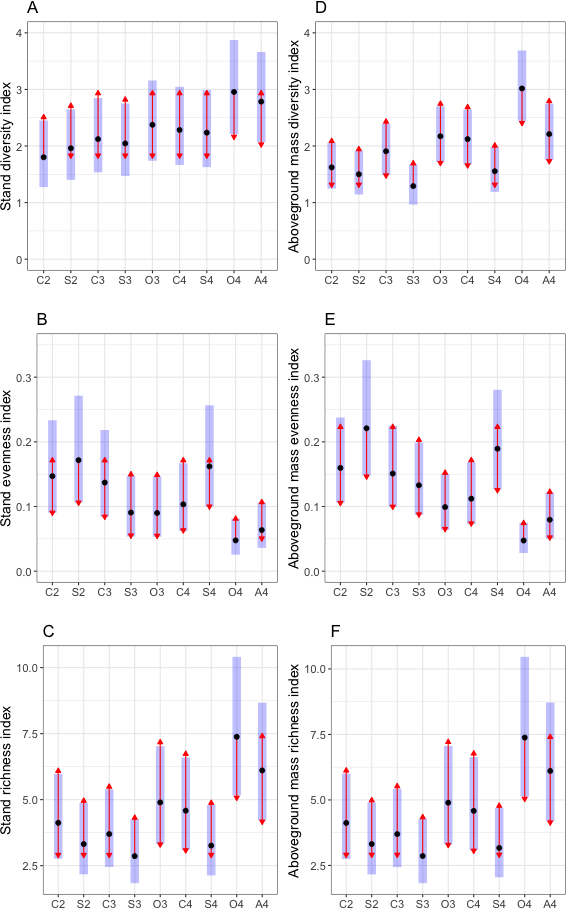
\includegraphics{Community_files/figure-latex/index-arrow-p-1.png}
\caption{\label{fig:index-arrow-p}Weed community stand diversity (A), evenness (B), and richness (C) and community aboveground diversity (D), evenness (E), and richness (F). The abbreviations on the x-axis are crop identities, which are the combinations of the first letter in crop species names and the rotation in which it occurred (C2 - corn in the 2-year rotation, C3 - corn in the 3-year rotation, C4 - corn in the 4-year rotation, S2 - soybean in the 2-year rotation, S3 - soybean in the 3-year rotation, S4 - soybean in the 4-year rotation, O3 - oat in the 3-year rotation, O4 - oat in the 4-year rotation, and A4 - alfalfa in the 4-year rotation). The black dots are estimated marginal means. The blue bars are 95\% confidence intervals. The red arrows reflect comparisons among means. Overlapping arrows indicate non-significant differences.}
\end{figure}

\emph{In general, the hypothesis that ``weed communities in the more diverse cropping systems are more diverse'' was supported.}

Averaged over crop phases within each rotation system (Table \ref{tab:dens-indices-ct}A), the weed community stand diversity index for the 3-year and 4-year rotation systems was comparable with that in the 2-year rotation (p = 0.0535 and p = 0.1575, respectively). For the individual crops (Table \ref{tab:dens-indices-ct}B), the weed stand density diversity index was comparable among rotations (p \textgreater{} 0.05). For different crop types (Table \ref{tab:dens-indices-ct}C), the weed community stand density diversity index in the average for the cool-season crops (O3, O4, and A4) was 1.2-fold greater than that in the average for the warm-season crops (C2, S2, C3, S3, C4, and S4) (p = 0.0145), but similar between the warm-season and cool-season crops in the same rotations (p = 0.4666 and p = 0.0987, respectively). The weed stand density diversity index was similar between oat and alfalfa (p = 0.7762).

Averaged over crop phases within the same rotation (Table \ref{tab:biom-indices-ct}A), the weed community aboveground mass diversity index was different between the 2-year rotation and the average of the 3-year and 4-year rotations (p = 0.0148), and between the 3-year and 4-year rotations (p = 0.0209). Averaged over the corn and soybean phases within the same rotation (Table \ref{tab:biom-indices-ct}A), the weed community aboveground mass diversity index was similar between rotations (p = 0.4217 and p = 0.2426, respectively). For the individual crops (Table \ref{tab:dens-indices-ct}B), the weed community aboveground mass diversity index was comparable between rotations, except for oat (p = 0.0351). For different crop types (Table \ref{tab:dens-indices-ct}C), the weed community aboveground mass diversity index in the cool-season crops average was 1.3-fold greater than that in the warm-season crops averages, overall (p \textless{} 0.0001), and was 1.23-fold and 1.27-fold greater in the cool-season than that in the warm-season crops in the 3-year (p = 0.034) and 4-year rotation (p = 0.0037), respectively. The weed community aboveground mass diversity index was comparable between oat and alfalfa (p = 0.2583).

\emph{The hypothesis that ``weed communities in the more diverse cropping systems are more even'' was partially supported (Figure \ref{fig:index-arrow-p}B and E).} However, a lower community evenness index can occur because the presence of rarer species decreases the overall evenness index {[}@stirlingEmpiricalRelationshipsSpecies2001{]}. More details to support this concept are presented later (Figure \ref{fig:all-sp-dens-biom}C and D).

Averaged over crop phases within the same rotation (Table \ref{tab:dens-indices-ct}A), the weed community stand density evenness index in the 2-year rotation was 1.6-fold greater than that in the average of the 3-year and 4-year rotations (p = 0.006), but comparable between the 3-year and 4-year rotations (p = 0.2802). Averaged over the corn and soybean phases within the same rotation (Table \ref{tab:dens-indices-ct}A), the weed community stand density evenness index was comparable between rotations (p = 0.1539 and p = 0.5031, respectively). For the individual crops (Table \ref{tab:dens-indices-ct}B), the weed community stand density evenness index was comparable between rotations (p \textgreater{} 0.05). For different crop types (Table \ref{tab:dens-indices-ct}C), the weed community stand density evenness index in the cool-season crops average was half of that in the warm-season crops average (p = 0.0002) and half of that in the cool-season and warm-season crop in the 4-year rotation (p = 0.0012), but similar between the warm-season and cool-season crops in the 3-year rotation (p = 0.4418). The weed community stand density evenness index was comparable between oat and alfalfa (p = 0.8986).

Averaged over crop phases within the same rotation (Table \ref{tab:biom-indices-ct}A), the weed community aboveground mass evenness index in the 2-year rotation was 1.65-fold greater than that in the average of 3-year and 4-year rotations (p = 0.0012), but similar between the 3-year and 4-year rotations (p = 0.0802). Averaged over the corn and soybean phases within the same rotation (Table \ref{tab:biom-indices-ct}A), weed community aboveground mass evenness index was comparable between rotations (p = 0.1081 and p = 0.8682, respectively). For the individual crops (Table \ref{tab:dens-indices-ct}B), the weed community aboveground mass evenness index was comparable between rotations (p \textgreater{} 0.05), except for oat (p = 0.0189). The weed community aboveground mass evenness index in the warm-season crops average was twice that of the cool-season crops average (p \textless{} 0.0001). The weed community aboveground mass evenness index in the warm-season crops was twice that of the cool-season crops in the 4-year rotation (p = 0.0002), but comparable between between the warm-season and cool-season crops in the 3-year rotation (p = 0.141), and between oat and alfalfa (p = 0.5911).

\emph{The hypothesis that ``the weed communities in the more diverse cropping systems are more species-rich'' was supported.}

Averaged over crop phases within the same rotation (Table \ref{tab:dens-indices-ct}A), the weed community stand density richness index was comparable in the 2-year rotation and in the average of the 3-year and 4-year rotations (p = 0.1819), but the stand density richness index in the 3-year was 0.77 that of the 4-year rotation (p = 0.0257). Averaged over the corn and soybean phases within the same rotation (Table \ref{tab:dens-indices-ct}A), weed community aboveground mass richness index was comparable between the 2-year rotation and the 3-year and 4-year rotations average (p = 0.7996) and between the 3-year and 4-year rotations (p = 0.3469). For individual crops (Table \ref{tab:dens-indices-ct}B), the weed community stand density richness index was comparable between rotations (p \textgreater{} 0.05). For different crop types (Table \ref{tab:dens-indices-ct}C), the weed stand density richness index in the cool-season crops average was 1.33-fold greater that of the warm-season crops average (p = 0.0003). Within the 4-year rotation, the weed stand density richness index in the cool-season was 1.58-fold greater than that in the warm-season crops (p = 0.0034). The weed stand density richness was comparable between the warm-season and cool-season crops in the 3-year rotation (p = 0.0725) and between oat and alfalfa (p = 0.9499).

The same patterns of difference and similarity of weed community richness index calculated with aboveground mass was observed (Table \ref{tab:biom-indices-ct}).

\subparagraph{Contrasts for ecological indices: diversity}\label{contrasts-for-ecological-indices-diversity}

\begin{Shaded}
\begin{Highlighting}[]
\DocumentationTok{\#\# Coefficients for customized contrasts }
\NormalTok{C2 }\OtherTok{\textless{}{-}} \FunctionTok{c}\NormalTok{(}\DecValTok{1}\NormalTok{,}\FunctionTok{rep}\NormalTok{(}\DecValTok{0}\NormalTok{,}\DecValTok{8}\NormalTok{)); C3 }\OtherTok{\textless{}{-}} \FunctionTok{c}\NormalTok{(}\DecValTok{0}\NormalTok{,}\DecValTok{0}\NormalTok{,}\DecValTok{1}\NormalTok{,}\FunctionTok{rep}\NormalTok{(}\DecValTok{0}\NormalTok{,}\DecValTok{6}\NormalTok{)); C4 }\OtherTok{\textless{}{-}} \FunctionTok{c}\NormalTok{(}\FunctionTok{rep}\NormalTok{(}\DecValTok{0}\NormalTok{,}\DecValTok{5}\NormalTok{),}\DecValTok{1}\NormalTok{,}\FunctionTok{rep}\NormalTok{(}\DecValTok{0}\NormalTok{,}\DecValTok{3}\NormalTok{))}
\NormalTok{S2 }\OtherTok{\textless{}{-}} \FunctionTok{c}\NormalTok{(}\DecValTok{0}\NormalTok{, }\DecValTok{1}\NormalTok{,}\FunctionTok{rep}\NormalTok{(}\DecValTok{0}\NormalTok{,}\DecValTok{7}\NormalTok{)); S3 }\OtherTok{\textless{}{-}} \FunctionTok{c}\NormalTok{(}\FunctionTok{rep}\NormalTok{(}\DecValTok{0}\NormalTok{,}\DecValTok{3}\NormalTok{), }\DecValTok{1}\NormalTok{,}\FunctionTok{rep}\NormalTok{(}\DecValTok{0}\NormalTok{,}\DecValTok{5}\NormalTok{)); S4 }\OtherTok{\textless{}{-}} \FunctionTok{c}\NormalTok{(}\FunctionTok{rep}\NormalTok{(}\DecValTok{0}\NormalTok{,}\DecValTok{6}\NormalTok{),}\DecValTok{1}\NormalTok{,}\FunctionTok{rep}\NormalTok{(}\DecValTok{0}\NormalTok{,}\DecValTok{2}\NormalTok{))}
\NormalTok{O3 }\OtherTok{\textless{}{-}} \FunctionTok{c}\NormalTok{(}\FunctionTok{rep}\NormalTok{(}\DecValTok{0}\NormalTok{,}\DecValTok{4}\NormalTok{), }\DecValTok{1}\NormalTok{, }\FunctionTok{rep}\NormalTok{(}\DecValTok{0}\NormalTok{,}\DecValTok{4}\NormalTok{)); O4 }\OtherTok{\textless{}{-}} \FunctionTok{c}\NormalTok{(}\FunctionTok{rep}\NormalTok{(}\DecValTok{0}\NormalTok{,}\DecValTok{7}\NormalTok{),}\DecValTok{1}\NormalTok{,}\DecValTok{0}\NormalTok{)}
\NormalTok{A4 }\OtherTok{\textless{}{-}} \FunctionTok{c}\NormalTok{(}\FunctionTok{rep}\NormalTok{(}\DecValTok{0}\NormalTok{,}\DecValTok{8}\NormalTok{), }\DecValTok{1}\NormalTok{)}


\DocumentationTok{\#\#\#\#\# Did rotation affect density diversity, average over all crop phases within the same rotation?}
\DocumentationTok{\#\# 2{-}year vs (3{-}year + 4{-}year)/2}
\NormalTok{dens\_diversity\_2yrvs34yr }\OtherTok{\textless{}{-}} \FunctionTok{print}\NormalTok{(}\FunctionTok{contrast}\NormalTok{(}\FunctionTok{emmeans}\NormalTok{(dens\_diversity.lmer1, }\SpecialCharTok{\textasciitilde{}}\NormalTok{ Crop\_ID,}
                                                   \AttributeTok{infer =} \FunctionTok{c}\NormalTok{(}\ConstantTok{FALSE}\NormalTok{,}\ConstantTok{TRUE}\NormalTok{), }
                                                   \AttributeTok{type =} \StringTok{"response"}\NormalTok{),}
                                           \AttributeTok{method =} \FunctionTok{list}\NormalTok{(}\StringTok{"[(C2+S2)/2] vs [(C3+S3+O3+C4+S4+O4+A4)/7]"} \OtherTok{=} 
\NormalTok{                                                           ((C2}\SpecialCharTok{+}\NormalTok{S2)}\SpecialCharTok{/}\DecValTok{2}\NormalTok{) }\SpecialCharTok{{-}}\NormalTok{ ((C3}\SpecialCharTok{+}\NormalTok{S3}\SpecialCharTok{+}\NormalTok{O3}\SpecialCharTok{+}\NormalTok{C4}\SpecialCharTok{+}\NormalTok{S4}\SpecialCharTok{+}\NormalTok{O4}\SpecialCharTok{+}\NormalTok{A4)}\SpecialCharTok{/}\DecValTok{7}\NormalTok{))),}
                                  \AttributeTok{export =} \ConstantTok{TRUE}\NormalTok{)}

\DocumentationTok{\#\# 3{-}year vs 4{-}year}
\NormalTok{dens\_diversity\_3yrvs4yr }\OtherTok{=} \FunctionTok{print}\NormalTok{(}\FunctionTok{contrast}\NormalTok{(}\FunctionTok{emmeans}\NormalTok{(dens\_diversity.lmer1, }\SpecialCharTok{\textasciitilde{}}\NormalTok{ Crop\_ID, }
                                                 \AttributeTok{infer =} \FunctionTok{c}\NormalTok{(}\ConstantTok{FALSE}\NormalTok{,}\ConstantTok{TRUE}\NormalTok{), }
                                                 \AttributeTok{type =} \StringTok{"response"}\NormalTok{),}
                                         \AttributeTok{method =} \FunctionTok{list}\NormalTok{(}\StringTok{"[(C3+S3+O3)/3] vs [(C4+S4+O4+A4)/4]"} \OtherTok{=} 
\NormalTok{                                                         ((C3}\SpecialCharTok{+}\NormalTok{S3}\SpecialCharTok{+}\NormalTok{O3)}\SpecialCharTok{/}\DecValTok{3}\NormalTok{) }\SpecialCharTok{{-}}\NormalTok{ ((C4}\SpecialCharTok{+}\NormalTok{S4}\SpecialCharTok{+}\NormalTok{O4}\SpecialCharTok{+}\NormalTok{A4)}\SpecialCharTok{/}\DecValTok{4}\NormalTok{) )), }
                                \AttributeTok{export =} \ConstantTok{TRUE}\NormalTok{)}
\DocumentationTok{\#\# 2{-}year vs 3{-}year }
\NormalTok{dens\_diversity\_2yrvs3yr }\OtherTok{\textless{}{-}} \FunctionTok{print}\NormalTok{(}\FunctionTok{contrast}\NormalTok{(}\FunctionTok{emmeans}\NormalTok{(dens\_diversity.lmer1, }\SpecialCharTok{\textasciitilde{}}\NormalTok{ Crop\_ID, }
                                                  \AttributeTok{infer =} \FunctionTok{c}\NormalTok{(}\ConstantTok{FALSE}\NormalTok{,}\ConstantTok{TRUE}\NormalTok{), }
                                                  \AttributeTok{type =} \StringTok{"response"}\NormalTok{),}
                                          \AttributeTok{method =} \FunctionTok{list}\NormalTok{(}\StringTok{"[(C2+S2)/2] vs [(C3+S3+O3)/3]"} \OtherTok{=} 
\NormalTok{                                                          ((C2}\SpecialCharTok{+}\NormalTok{S2)}\SpecialCharTok{/}\DecValTok{2}\NormalTok{) }\SpecialCharTok{{-}}\NormalTok{ ((C3}\SpecialCharTok{+}\NormalTok{S3}\SpecialCharTok{+}\NormalTok{O3)}\SpecialCharTok{/}\DecValTok{3}\NormalTok{) )),}
                                 \AttributeTok{export =} \ConstantTok{TRUE}\NormalTok{)}

\DocumentationTok{\#\# 2{-}year vs 4{-}year }
\NormalTok{dens\_diversity\_2yrvs4yr }\OtherTok{=} \FunctionTok{print}\NormalTok{(}\FunctionTok{contrast}\NormalTok{(}\FunctionTok{emmeans}\NormalTok{(dens\_diversity.lmer1, }\SpecialCharTok{\textasciitilde{}}\NormalTok{ Crop\_ID,}
                                                 \AttributeTok{infer =} \FunctionTok{c}\NormalTok{(}\ConstantTok{FALSE}\NormalTok{,}\ConstantTok{TRUE}\NormalTok{),  }
                                                 \AttributeTok{type =} \StringTok{"response"}\NormalTok{), }
                                         \AttributeTok{method =} \FunctionTok{list}\NormalTok{(}\StringTok{"[(C2+S2)/2] vs [(C4+S4+O4+A4)/4]"} \OtherTok{=} 
\NormalTok{                                                         ((C2}\SpecialCharTok{+}\NormalTok{S2)}\SpecialCharTok{/}\DecValTok{2}\NormalTok{) }\SpecialCharTok{{-}}\NormalTok{ ((C4}\SpecialCharTok{+}\NormalTok{S4}\SpecialCharTok{+}\NormalTok{O4}\SpecialCharTok{+}\NormalTok{A4)}\SpecialCharTok{/}\DecValTok{4}\NormalTok{) )), }
                                \AttributeTok{export =} \ConstantTok{TRUE}\NormalTok{)}


\DocumentationTok{\#\# Corn and soybean average: (C2+S2)/2 vs. (C3+S3+C4+S4)/4}
\NormalTok{dens\_diversity\_CS2yr\_vs\_CS34yr }\OtherTok{\textless{}{-}} \FunctionTok{print}\NormalTok{(}\FunctionTok{contrast}\NormalTok{(}\FunctionTok{emmeans}\NormalTok{(dens\_diversity.lmer1, }\SpecialCharTok{\textasciitilde{}}\NormalTok{ Crop\_ID,}
                                                         \AttributeTok{infer =} \FunctionTok{c}\NormalTok{(}\ConstantTok{FALSE}\NormalTok{,}\ConstantTok{TRUE}\NormalTok{),}
                                                         \AttributeTok{type =} \StringTok{"response"}\NormalTok{), }
                                                 \AttributeTok{method =} \FunctionTok{list}\NormalTok{(}\StringTok{"[(C2+S2)/2] vs [(C3+S3+C4+S4)/4]"} \OtherTok{=} 
\NormalTok{                                                                 ((C2}\SpecialCharTok{+}\NormalTok{S2)}\SpecialCharTok{/}\DecValTok{2}\NormalTok{) }\SpecialCharTok{{-}}\NormalTok{ ((C3}\SpecialCharTok{+}\NormalTok{S3}\SpecialCharTok{+}\NormalTok{C4}\SpecialCharTok{+}\NormalTok{S4)}\SpecialCharTok{/}\DecValTok{4}\NormalTok{) )),}
                                        \AttributeTok{export =} \ConstantTok{TRUE}\NormalTok{)}

\DocumentationTok{\#\# Corn and soybean average: (C3+S3)/2 vs. C4+S4)/2}
\NormalTok{dens\_diversity\_CS3yr\_vs\_CS4yr }\OtherTok{\textless{}{-}} \FunctionTok{print}\NormalTok{(}\FunctionTok{contrast}\NormalTok{(}\FunctionTok{emmeans}\NormalTok{(dens\_diversity.lmer1, }\SpecialCharTok{\textasciitilde{}}\NormalTok{ Crop\_ID,}
                                                        \AttributeTok{infer =} \FunctionTok{c}\NormalTok{(}\ConstantTok{FALSE}\NormalTok{,}\ConstantTok{TRUE}\NormalTok{), }
                                                        \AttributeTok{type =} \StringTok{"response"}\NormalTok{),}
                                                \AttributeTok{method =} \FunctionTok{list}\NormalTok{(}\StringTok{"[(C3+S3)/2] vs [(C4+S4)/2]"} \OtherTok{=}
\NormalTok{                                                                ((C3}\SpecialCharTok{+}\NormalTok{S3)}\SpecialCharTok{/}\DecValTok{2}\NormalTok{) }\SpecialCharTok{{-}}\NormalTok{ ((C4}\SpecialCharTok{+}\NormalTok{S4)}\SpecialCharTok{/}\DecValTok{2}\NormalTok{) )),}
                                       \AttributeTok{export =} \ConstantTok{TRUE}\NormalTok{)}


\DocumentationTok{\#\#\#\#\# Did crop species affect density diversity, across rotations?}

\DocumentationTok{\#\#\#\# 3yr: summer vs. cool{-}season crops: (C3+S3)/2 vs. O3}
\NormalTok{dens\_diversity\_CS3\_vs\_O3 }\OtherTok{\textless{}{-}} \FunctionTok{print}\NormalTok{(}\FunctionTok{contrast}\NormalTok{(}\FunctionTok{emmeans}\NormalTok{(dens\_diversity.lmer1, }\SpecialCharTok{\textasciitilde{}}\NormalTok{ Crop\_ID, }
                                                   \AttributeTok{infer =} \FunctionTok{c}\NormalTok{(}\ConstantTok{FALSE}\NormalTok{,}\ConstantTok{TRUE}\NormalTok{), }
                                                   \AttributeTok{type =} \StringTok{"response"}\NormalTok{),}
                                           \AttributeTok{method =} \FunctionTok{list}\NormalTok{(}\StringTok{"O3 vs [(C3+S3)/2]"} \OtherTok{=}\NormalTok{ O3 }\SpecialCharTok{{-}}\NormalTok{ (C3}\SpecialCharTok{+}\NormalTok{S3)}\SpecialCharTok{/}\DecValTok{2}\NormalTok{)),}
                                  \AttributeTok{export =} \ConstantTok{TRUE}\NormalTok{)}

\DocumentationTok{\#\#\#\# 4yr: summer vs. cool{-}season crops: (C4+S4)/2 vs. (O4+A4)/2 }
\NormalTok{dens\_diversity\_CS4\_vs\_OA4 }\OtherTok{\textless{}{-}} \FunctionTok{print}\NormalTok{(}\FunctionTok{contrast}\NormalTok{(}\FunctionTok{emmeans}\NormalTok{(dens\_diversity.lmer1, }\SpecialCharTok{\textasciitilde{}}\NormalTok{ Crop\_ID,}
                                                    \AttributeTok{infer =} \FunctionTok{c}\NormalTok{(}\ConstantTok{FALSE}\NormalTok{,}\ConstantTok{TRUE}\NormalTok{),}
                                                    \AttributeTok{type =} \StringTok{"response"}\NormalTok{), }
                                            \AttributeTok{method =} \FunctionTok{list}\NormalTok{(}\StringTok{"[(O4+A4)/2] vs [(C4+S4)/2]"} \OtherTok{=} 
\NormalTok{                                                            ((A4}\SpecialCharTok{+}\NormalTok{O4)}\SpecialCharTok{/}\DecValTok{2}\NormalTok{) }\SpecialCharTok{{-}}\NormalTok{ ((C4}\SpecialCharTok{+}\NormalTok{S4)}\SpecialCharTok{/}\DecValTok{2}\NormalTok{))), }
                                   \AttributeTok{export =} \ConstantTok{TRUE}\NormalTok{)}

\DocumentationTok{\#\#\#\# all summer vs. all cool{-}season crops: }
\NormalTok{dens\_diversity\_summer\_vs\_cool }\OtherTok{\textless{}{-}} \FunctionTok{print}\NormalTok{(}\FunctionTok{contrast}\NormalTok{(}\FunctionTok{emmeans}\NormalTok{(dens\_diversity.lmer1, }\SpecialCharTok{\textasciitilde{}}\NormalTok{ Crop\_ID, }
                                                        \AttributeTok{infer =} \FunctionTok{c}\NormalTok{(}\ConstantTok{FALSE}\NormalTok{,}\ConstantTok{TRUE}\NormalTok{),}
                                                        \AttributeTok{type =} \StringTok{"response"}\NormalTok{),}
                                                \AttributeTok{method =} \FunctionTok{list}\NormalTok{(}\StringTok{"[(O3+O4+A4)/3] vs [(C2+S2+C3+S3+C4+S4)/6]"} \OtherTok{=}
\NormalTok{                                                                 ((O3}\SpecialCharTok{+}\NormalTok{A4}\SpecialCharTok{+}\NormalTok{O4)}\SpecialCharTok{/}\DecValTok{3}\NormalTok{) }\SpecialCharTok{{-}}\NormalTok{ ((C2}\SpecialCharTok{+}\NormalTok{S2}\SpecialCharTok{+}\NormalTok{C3}\SpecialCharTok{+}\NormalTok{S3}\SpecialCharTok{+}\NormalTok{C4}\SpecialCharTok{+}\NormalTok{S4)}\SpecialCharTok{/}\DecValTok{6}\NormalTok{)) ), }
                                       \AttributeTok{export =} \ConstantTok{TRUE}\NormalTok{)}

\DocumentationTok{\#\#\#\# Did rotation affect diversity in density composition for the communities grew in the same crop species?  }
\CommentTok{\# Corn: C2 vs (C3+C4)/2 }
\NormalTok{dens\_diversity\_C2vs3\_4 }\OtherTok{\textless{}{-}} \FunctionTok{print}\NormalTok{(}\FunctionTok{contrast}\NormalTok{(}\FunctionTok{emmeans}\NormalTok{(dens\_diversity.lmer1, }\SpecialCharTok{\textasciitilde{}}\NormalTok{ Crop\_ID, }
                                                 \AttributeTok{infer =} \FunctionTok{c}\NormalTok{(}\ConstantTok{FALSE}\NormalTok{,}\ConstantTok{TRUE}\NormalTok{),}
                                                 \AttributeTok{type =} \StringTok{"response"}\NormalTok{),}
                                         \AttributeTok{method =} \FunctionTok{list}\NormalTok{(}\StringTok{"C2 vs [(C3+C4)/2]"} \OtherTok{=}\NormalTok{ C2 }\SpecialCharTok{{-}}\NormalTok{ ((C3}\SpecialCharTok{+}\NormalTok{C4)}\SpecialCharTok{/}\DecValTok{2}\NormalTok{) )),}
                                \AttributeTok{export =} \ConstantTok{TRUE}\NormalTok{)}
\CommentTok{\# Corn: C3 vs C4}
\NormalTok{dens\_diversity\_C3vs4 }\OtherTok{\textless{}{-}} \FunctionTok{print}\NormalTok{(}\FunctionTok{contrast}\NormalTok{(}\FunctionTok{emmeans}\NormalTok{(dens\_diversity.lmer1, }\SpecialCharTok{\textasciitilde{}}\NormalTok{ Crop\_ID,}
                                               \AttributeTok{infer =} \FunctionTok{c}\NormalTok{(}\ConstantTok{FALSE}\NormalTok{,}\ConstantTok{TRUE}\NormalTok{), }
                                               \AttributeTok{type =} \StringTok{"response"}\NormalTok{,}
                                               \AttributeTok{at =} \FunctionTok{list}\NormalTok{(}\AttributeTok{Crop\_ID =} \FunctionTok{c}\NormalTok{( }\StringTok{"C3"}\NormalTok{, }\StringTok{"C4"}\NormalTok{))), }\StringTok{"pairwise"}\NormalTok{),}
                              \AttributeTok{export =} \ConstantTok{TRUE}\NormalTok{) }\CommentTok{\#not included in the final table}


\CommentTok{\# Soybean: S2 vs (S3+S4)/2 }
\NormalTok{dens\_diversity\_S2vs3\_4 }\OtherTok{\textless{}{-}} \FunctionTok{print}\NormalTok{(}\FunctionTok{contrast}\NormalTok{(}\FunctionTok{emmeans}\NormalTok{(dens\_diversity.lmer1, }\SpecialCharTok{\textasciitilde{}}\NormalTok{ Crop\_ID, }
                                                 \AttributeTok{infer =} \FunctionTok{c}\NormalTok{(}\ConstantTok{FALSE}\NormalTok{,}\ConstantTok{TRUE}\NormalTok{), }
                                                 \AttributeTok{type =} \StringTok{"response"}\NormalTok{), }
                                         \AttributeTok{method =} \FunctionTok{list}\NormalTok{(}\StringTok{"S2 vs [(S3+S4)/2]"} \OtherTok{=}\NormalTok{ S2 }\SpecialCharTok{{-}}\NormalTok{ ((S3}\SpecialCharTok{+}\NormalTok{S4)}\SpecialCharTok{/}\DecValTok{2}\NormalTok{) )), }
                                \AttributeTok{export =} \ConstantTok{TRUE}\NormalTok{)}

\CommentTok{\# Soybean: S3 vs S4}
\NormalTok{dens\_diversity\_S3vs4 }\OtherTok{\textless{}{-}}\FunctionTok{print}\NormalTok{(}\FunctionTok{contrast}\NormalTok{(}\FunctionTok{emmeans}\NormalTok{(dens\_diversity.lmer1, }\SpecialCharTok{\textasciitilde{}}\NormalTok{ Crop\_ID,}
                                              \AttributeTok{infer =} \FunctionTok{c}\NormalTok{(}\ConstantTok{FALSE}\NormalTok{,}\ConstantTok{TRUE}\NormalTok{), }
                                              \AttributeTok{type =} \StringTok{"response"}\NormalTok{,}
                                              \AttributeTok{at =} \FunctionTok{list}\NormalTok{(}\AttributeTok{Crop\_ID =} \FunctionTok{c}\NormalTok{( }\StringTok{"S3"}\NormalTok{, }\StringTok{"S4"}\NormalTok{))), }\StringTok{"pairwise"}\NormalTok{),}
                             \AttributeTok{export =} \ConstantTok{TRUE}\NormalTok{) }\CommentTok{\#not included in the final table}


\CommentTok{\# Oat: O3 vs O4}
\NormalTok{dens\_diversity\_oat }\OtherTok{\textless{}{-}} \FunctionTok{print}\NormalTok{(}\FunctionTok{contrast}\NormalTok{(}\FunctionTok{emmeans}\NormalTok{(dens\_diversity.lmer1, }\SpecialCharTok{\textasciitilde{}}\NormalTok{ Crop\_ID,}
                                             \AttributeTok{infer =} \FunctionTok{c}\NormalTok{(}\ConstantTok{FALSE}\NormalTok{,}\ConstantTok{TRUE}\NormalTok{), }
                                             \AttributeTok{type =} \StringTok{"response"}\NormalTok{, }
                                             \AttributeTok{at =} \FunctionTok{list}\NormalTok{(}\AttributeTok{Crop\_ID =} \FunctionTok{c}\NormalTok{(}\StringTok{"O3"}\NormalTok{, }\StringTok{"O4"}\NormalTok{))), }\StringTok{"pairwise"}\NormalTok{), }
                            \AttributeTok{export =} \ConstantTok{TRUE}\NormalTok{)}

\CommentTok{\# oat vs alfalfa}
\NormalTok{dens\_diversity\_OA }\OtherTok{\textless{}{-}} \FunctionTok{print}\NormalTok{(}\FunctionTok{contrast}\NormalTok{(}\FunctionTok{emmeans}\NormalTok{(dens\_diversity.lmer1, }\SpecialCharTok{\textasciitilde{}}\NormalTok{ Crop\_ID,}
                                            \AttributeTok{infer =} \FunctionTok{c}\NormalTok{(}\ConstantTok{FALSE}\NormalTok{,}\ConstantTok{TRUE}\NormalTok{), }
                                            \AttributeTok{type =} \StringTok{"response"}\NormalTok{), }
                                    \AttributeTok{method =} \FunctionTok{list}\NormalTok{(}\StringTok{"[(O3+O4)/2] vs A4"} \OtherTok{=}\NormalTok{ ( ((O3}\SpecialCharTok{+}\NormalTok{O4)}\SpecialCharTok{/}\DecValTok{2}\NormalTok{)) }\SpecialCharTok{{-}}\NormalTok{ A4)),}
                           \AttributeTok{export =} \ConstantTok{TRUE}\NormalTok{)}


\DocumentationTok{\#\#\#\#\#\# Biomass \#\#\#\#\#\#\#}
\DocumentationTok{\#\#\#\#\# Did rotation affect density diversity, average over all crop phases within the same rotation?}

\CommentTok{\#2{-}year vs (3{-}year + 4{-}year)/2}
\NormalTok{biom\_diversity\_2yrvs34yr }\OtherTok{\textless{}{-}} \FunctionTok{print}\NormalTok{(}\FunctionTok{contrast}\NormalTok{(}\FunctionTok{emmeans}\NormalTok{(biom\_diversity.lmer1, }\SpecialCharTok{\textasciitilde{}}\NormalTok{ Crop\_ID,}
                                                   \AttributeTok{infer =} \FunctionTok{c}\NormalTok{(}\ConstantTok{FALSE}\NormalTok{,}\ConstantTok{TRUE}\NormalTok{), }
                                                   \AttributeTok{type =} \StringTok{"response"}\NormalTok{),}
                                           \AttributeTok{method =} \FunctionTok{list}\NormalTok{(}\StringTok{"[(C2+S2)/2] vs [(C3+S3+O3+C4+S4+O4+A4)/7]"} \OtherTok{=} 
\NormalTok{                                                           (C2}\SpecialCharTok{+}\NormalTok{S2)}\SpecialCharTok{/}\DecValTok{2} \SpecialCharTok{{-}}\NormalTok{ (C3}\SpecialCharTok{+}\NormalTok{S3}\SpecialCharTok{+}\NormalTok{O3}\SpecialCharTok{+}\NormalTok{C4}\SpecialCharTok{+}\NormalTok{S4}\SpecialCharTok{+}\NormalTok{O4}\SpecialCharTok{+}\NormalTok{A4)}\SpecialCharTok{/}\DecValTok{7}\NormalTok{ )),}
                                  \AttributeTok{export =} \ConstantTok{TRUE}\NormalTok{)}

\CommentTok{\#3{-}year vs 4{-}year average}
\NormalTok{biom\_diversity\_3yrvs4yr }\OtherTok{=} \FunctionTok{print}\NormalTok{(}\FunctionTok{contrast}\NormalTok{(}\FunctionTok{emmeans}\NormalTok{(biom\_diversity.lmer1, }\SpecialCharTok{\textasciitilde{}}\NormalTok{ Crop\_ID,}
                                                 \AttributeTok{infer =} \FunctionTok{c}\NormalTok{(}\ConstantTok{FALSE}\NormalTok{,}\ConstantTok{TRUE}\NormalTok{), }
                                                 \AttributeTok{type =} \StringTok{"response"}\NormalTok{), }
                                         \AttributeTok{method =} \FunctionTok{list}\NormalTok{(}\StringTok{"[(C3+S3+O3)/3] vs [(C4+S4+O4+A4)/4]"} \OtherTok{=} 
\NormalTok{                                                         ((C3}\SpecialCharTok{+}\NormalTok{S3}\SpecialCharTok{+}\NormalTok{O3)}\SpecialCharTok{/}\DecValTok{3}\NormalTok{) }\SpecialCharTok{{-}}\NormalTok{ ((C4}\SpecialCharTok{+}\NormalTok{S4}\SpecialCharTok{+}\NormalTok{O4}\SpecialCharTok{+}\NormalTok{A4)}\SpecialCharTok{/}\DecValTok{4}\NormalTok{) )),}
                                \AttributeTok{export =} \ConstantTok{TRUE}\NormalTok{)}

\CommentTok{\#2{-}year vs 3{-}year average}
\NormalTok{biom\_diversity\_2yrvs3yr }\OtherTok{\textless{}{-}} \FunctionTok{print}\NormalTok{(}\FunctionTok{contrast}\NormalTok{(}\FunctionTok{emmeans}\NormalTok{(biom\_diversity.lmer1, }\SpecialCharTok{\textasciitilde{}}\NormalTok{ Crop\_ID,}
                                                  \AttributeTok{infer =} \FunctionTok{c}\NormalTok{(}\ConstantTok{FALSE}\NormalTok{,}\ConstantTok{TRUE}\NormalTok{),}
                                                  \AttributeTok{type =} \StringTok{"response"}\NormalTok{),}
                                          \AttributeTok{method =} \FunctionTok{list}\NormalTok{(}\StringTok{"[(C2+S2)/2] vs [(C3+S3+O3)/3]"} \OtherTok{=} 
\NormalTok{                                                          ((C2}\SpecialCharTok{+}\NormalTok{S2)}\SpecialCharTok{/}\DecValTok{2}\NormalTok{) }\SpecialCharTok{{-}}\NormalTok{ ((C3}\SpecialCharTok{+}\NormalTok{S3}\SpecialCharTok{+}\NormalTok{O3)}\SpecialCharTok{/}\DecValTok{3}\NormalTok{) )), }
                                 \AttributeTok{export =} \ConstantTok{TRUE}\NormalTok{)}

\CommentTok{\#2{-}year vs 4{-}year average}
\NormalTok{biom\_diversity\_2yrvs4yr }\OtherTok{=} \FunctionTok{print}\NormalTok{(}\FunctionTok{contrast}\NormalTok{(}\FunctionTok{emmeans}\NormalTok{(biom\_diversity.lmer1, }\SpecialCharTok{\textasciitilde{}}\NormalTok{ Crop\_ID, }
                                                 \AttributeTok{infer =} \FunctionTok{c}\NormalTok{(}\ConstantTok{FALSE}\NormalTok{,}\ConstantTok{TRUE}\NormalTok{), }
                                                 \AttributeTok{type =} \StringTok{"response"}\NormalTok{),}
                                         \AttributeTok{method =} \FunctionTok{list}\NormalTok{(}\StringTok{"[(C2+S2)/2] vs [(C4+S4+O4+A4)/4]"} \OtherTok{=}
\NormalTok{                                                         ((C2}\SpecialCharTok{+}\NormalTok{S2)}\SpecialCharTok{/}\DecValTok{2}\NormalTok{) }\SpecialCharTok{{-}}\NormalTok{ ((C4}\SpecialCharTok{+}\NormalTok{S4}\SpecialCharTok{+}\NormalTok{O4}\SpecialCharTok{+}\NormalTok{A4)}\SpecialCharTok{/}\DecValTok{4}\NormalTok{) )),}
                                \AttributeTok{export =} \ConstantTok{TRUE}\NormalTok{)}

\CommentTok{\#Corn and soybean average: (C2+S2)/2 vs. (C3+S3+C4+S4)/4}
\NormalTok{biom\_diversity\_CS2yr\_vs\_CS34yr }\OtherTok{\textless{}{-}} \FunctionTok{print}\NormalTok{(}\FunctionTok{contrast}\NormalTok{(}\FunctionTok{emmeans}\NormalTok{(biom\_diversity.lmer1, }\SpecialCharTok{\textasciitilde{}}\NormalTok{ Crop\_ID,}
                                                         \AttributeTok{infer =} \FunctionTok{c}\NormalTok{(}\ConstantTok{FALSE}\NormalTok{,}\ConstantTok{TRUE}\NormalTok{), }
                                                         \AttributeTok{type =} \StringTok{"response"}\NormalTok{),}
                                                 \AttributeTok{method =} \FunctionTok{list}\NormalTok{(}\StringTok{"[(C2+S2)/2] vs [(C3+S3+C4+S4)/4]"} \OtherTok{=} 
\NormalTok{                                                                 ((C2}\SpecialCharTok{+}\NormalTok{S2)}\SpecialCharTok{/}\DecValTok{2}\NormalTok{) }\SpecialCharTok{{-}}\NormalTok{ ((C3}\SpecialCharTok{+}\NormalTok{S3}\SpecialCharTok{+}\NormalTok{C4}\SpecialCharTok{+}\NormalTok{S4))}\SpecialCharTok{/}\DecValTok{4}\NormalTok{)),}
                                        \AttributeTok{export =} \ConstantTok{TRUE}\NormalTok{)}

\DocumentationTok{\#\# Corn and soybean average: (C3+S3)/2 vs. C4+S4)/2}
\NormalTok{biom\_diversity\_CS3yr\_vs\_CS4yr }\OtherTok{\textless{}{-}} \FunctionTok{print}\NormalTok{(}\FunctionTok{contrast}\NormalTok{(}\FunctionTok{emmeans}\NormalTok{(biom\_diversity.lmer1, }\SpecialCharTok{\textasciitilde{}}\NormalTok{ Crop\_ID,}
                                                        \AttributeTok{infer =} \FunctionTok{c}\NormalTok{(}\ConstantTok{FALSE}\NormalTok{,}\ConstantTok{TRUE}\NormalTok{), }
                                                        \AttributeTok{type =} \StringTok{"response"}\NormalTok{), }
                                                \AttributeTok{method =} \FunctionTok{list}\NormalTok{(}\StringTok{"[(C3+S3)/2] vs [(C4+S4)/2]"} \OtherTok{=} 
\NormalTok{                                                                ((C3}\SpecialCharTok{+}\NormalTok{S3)}\SpecialCharTok{/}\DecValTok{2}\NormalTok{) }\SpecialCharTok{{-}}\NormalTok{ ((C4}\SpecialCharTok{+}\NormalTok{S4)}\SpecialCharTok{/}\DecValTok{2}\NormalTok{))),}
                                       \AttributeTok{export =} \ConstantTok{TRUE}\NormalTok{)}


\DocumentationTok{\#\#\#\#\#\#\# Does crop species affect biomass diversity, different crops, averaged across rotations}
\NormalTok{biom\_diversity\_CS3\_vs\_O3 }\OtherTok{\textless{}{-}} \FunctionTok{print}\NormalTok{(}\FunctionTok{contrast}\NormalTok{(}\FunctionTok{emmeans}\NormalTok{(biom\_diversity.lmer1, }\SpecialCharTok{\textasciitilde{}}\NormalTok{ Crop\_ID,}
                                                   \AttributeTok{infer =} \FunctionTok{c}\NormalTok{(}\ConstantTok{FALSE}\NormalTok{,}\ConstantTok{TRUE}\NormalTok{), }
                                                   \AttributeTok{type =} \StringTok{"response"}\NormalTok{),}
                                           \AttributeTok{method =} \FunctionTok{list}\NormalTok{(}\StringTok{"O3 vs [(C3+S3)/2]"} \OtherTok{=}\NormalTok{ O3 }\SpecialCharTok{{-}}\NormalTok{ (C3}\SpecialCharTok{+}\NormalTok{S3)}\SpecialCharTok{/}\DecValTok{2}\NormalTok{)),}
                                  \AttributeTok{export =} \ConstantTok{TRUE}\NormalTok{)}

\DocumentationTok{\#\#\#\# 4yr: summer vs. cool{-}season crops}
\DocumentationTok{\#\# (C4+S4)/2 vs. (O4+A4)/2 }
\NormalTok{biom\_diversity\_CS4\_vs\_OA4 }\OtherTok{\textless{}{-}} \FunctionTok{print}\NormalTok{(}\FunctionTok{contrast}\NormalTok{(}\FunctionTok{emmeans}\NormalTok{(biom\_diversity.lmer1, }\SpecialCharTok{\textasciitilde{}}\NormalTok{ Crop\_ID,}
                                                    \AttributeTok{infer =} \FunctionTok{c}\NormalTok{(}\ConstantTok{FALSE}\NormalTok{,}\ConstantTok{TRUE}\NormalTok{),  }
                                                    \AttributeTok{type =} \StringTok{"response"}\NormalTok{),}
                                            \AttributeTok{method =} \FunctionTok{list}\NormalTok{(}\StringTok{"[(O4+A4)/2] vs [(C4+S4)/2]"} \OtherTok{=}
\NormalTok{                                                            ((A4}\SpecialCharTok{+}\NormalTok{O4)}\SpecialCharTok{/}\DecValTok{2}\NormalTok{) }\SpecialCharTok{{-}}\NormalTok{ ((C4}\SpecialCharTok{+}\NormalTok{S4)}\SpecialCharTok{/}\DecValTok{2}\NormalTok{))),}
                                   \AttributeTok{export =} \ConstantTok{TRUE}\NormalTok{)}

\DocumentationTok{\#\#\#\# all summer vs. all cool{-}season crops }
\NormalTok{biom\_diversity\_summer\_vs\_cool }\OtherTok{\textless{}{-}} \FunctionTok{print}\NormalTok{(}\FunctionTok{contrast}\NormalTok{(}\FunctionTok{emmeans}\NormalTok{(biom\_diversity.lmer1, }\SpecialCharTok{\textasciitilde{}}\NormalTok{ Crop\_ID, }
                                                        \AttributeTok{infer =} \FunctionTok{c}\NormalTok{(}\ConstantTok{FALSE}\NormalTok{,}\ConstantTok{TRUE}\NormalTok{), }
                                                        \AttributeTok{type =} \StringTok{"response"}\NormalTok{),}
                                                \AttributeTok{method =} \FunctionTok{list}\NormalTok{(}\StringTok{"[(O3+O4+A4)/3] vs [(C2+S2+C3+S3+C4+S4)/6]"} \OtherTok{=} 
\NormalTok{                                                                 ((O3}\SpecialCharTok{+}\NormalTok{A4}\SpecialCharTok{+}\NormalTok{O4)}\SpecialCharTok{/}\DecValTok{3}\NormalTok{) }\SpecialCharTok{{-}}\NormalTok{ ((C2}\SpecialCharTok{+}\NormalTok{S2}\SpecialCharTok{+}\NormalTok{C3}\SpecialCharTok{+}\NormalTok{S3}\SpecialCharTok{+}\NormalTok{C4}\SpecialCharTok{+}\NormalTok{S4)}\SpecialCharTok{/}\DecValTok{6}\NormalTok{))) ,}
                                       \AttributeTok{export =} \ConstantTok{TRUE}\NormalTok{)}


\CommentTok{\# Corn: C2 vs (C3+C4)/2 }

\NormalTok{biom\_diversity\_C2vs3\_4 }\OtherTok{\textless{}{-}} \FunctionTok{print}\NormalTok{(}\FunctionTok{contrast}\NormalTok{(}\FunctionTok{emmeans}\NormalTok{(biom\_diversity.lmer1, }\SpecialCharTok{\textasciitilde{}}\NormalTok{ Crop\_ID,}
                                                 \AttributeTok{infer =} \FunctionTok{c}\NormalTok{(}\ConstantTok{FALSE}\NormalTok{,}\ConstantTok{TRUE}\NormalTok{), }
                                                 \AttributeTok{type =} \StringTok{"response"}\NormalTok{),}
                                         \AttributeTok{method =} \FunctionTok{list}\NormalTok{(}\StringTok{"C2 vs [(C3+C4)/2]"} \OtherTok{=}\NormalTok{ C2 }\SpecialCharTok{{-}}\NormalTok{ ((C3}\SpecialCharTok{+}\NormalTok{C4)}\SpecialCharTok{/}\DecValTok{2}\NormalTok{) )),}
                                \AttributeTok{export =} \ConstantTok{TRUE}\NormalTok{)}
\CommentTok{\# Corn: C3 vs C4}
\NormalTok{biom\_diversity\_C3vs4 }\OtherTok{\textless{}{-}} \FunctionTok{print}\NormalTok{(}\FunctionTok{contrast}\NormalTok{(}\FunctionTok{emmeans}\NormalTok{(biom\_diversity.lmer1, }\SpecialCharTok{\textasciitilde{}}\NormalTok{ Crop\_ID,}
                                               \AttributeTok{infer =} \FunctionTok{c}\NormalTok{(}\ConstantTok{FALSE}\NormalTok{,}\ConstantTok{TRUE}\NormalTok{), }
                                               \AttributeTok{type =} \StringTok{"response"}\NormalTok{, }
                                               \AttributeTok{at =} \FunctionTok{list}\NormalTok{(}\AttributeTok{Crop\_ID =} \FunctionTok{c}\NormalTok{( }\StringTok{"C3"}\NormalTok{, }\StringTok{"C4"}\NormalTok{))), }\StringTok{"pairwise"}\NormalTok{),}
                              \AttributeTok{export =} \ConstantTok{TRUE}\NormalTok{) }\CommentTok{\#not included in the final table}

\CommentTok{\# S2 vs (S3+S4)/2 and S3 vs S4}
\NormalTok{biom\_diversity\_S2vs3\_4 }\OtherTok{\textless{}{-}} \FunctionTok{print}\NormalTok{(}\FunctionTok{contrast}\NormalTok{(}\FunctionTok{emmeans}\NormalTok{(biom\_diversity.lmer1, }\SpecialCharTok{\textasciitilde{}}\NormalTok{ Crop\_ID,}
                                                 \AttributeTok{infer =} \FunctionTok{c}\NormalTok{(}\ConstantTok{FALSE}\NormalTok{,}\ConstantTok{TRUE}\NormalTok{), }
                                                 \AttributeTok{type =} \StringTok{"response"}\NormalTok{),}
                                         \AttributeTok{method =} \FunctionTok{list}\NormalTok{(}\StringTok{"S2 vs [(S3+S4)/2]"} \OtherTok{=}\NormalTok{ S2 }\SpecialCharTok{{-}}\NormalTok{ ((S3}\SpecialCharTok{+}\NormalTok{S4)}\SpecialCharTok{/}\DecValTok{2}\NormalTok{) )),}
                                \AttributeTok{export =} \ConstantTok{TRUE}\NormalTok{)}

\NormalTok{biom\_diversity\_S3vs4 }\OtherTok{\textless{}{-}}\FunctionTok{print}\NormalTok{(}\FunctionTok{contrast}\NormalTok{(}\FunctionTok{emmeans}\NormalTok{(biom\_diversity.lmer1, }\SpecialCharTok{\textasciitilde{}}\NormalTok{ Crop\_ID, }
                                              \AttributeTok{infer =} \FunctionTok{c}\NormalTok{(}\ConstantTok{FALSE}\NormalTok{,}\ConstantTok{TRUE}\NormalTok{), }
                                              \AttributeTok{type =} \StringTok{"response"}\NormalTok{, }
                                              \AttributeTok{at =} \FunctionTok{list}\NormalTok{(}\AttributeTok{Crop\_ID =} \FunctionTok{c}\NormalTok{( }\StringTok{"S3"}\NormalTok{, }\StringTok{"S4"}\NormalTok{))), }\StringTok{"pairwise"}\NormalTok{),}
                             \AttributeTok{export =} \ConstantTok{TRUE}\NormalTok{) }\CommentTok{\#not included in the final table}


\CommentTok{\# O3 vs O4}
\NormalTok{biom\_diversity\_oat }\OtherTok{\textless{}{-}} \FunctionTok{print}\NormalTok{(}\FunctionTok{contrast}\NormalTok{(}\FunctionTok{emmeans}\NormalTok{(biom\_diversity.lmer1, }\SpecialCharTok{\textasciitilde{}}\NormalTok{ Crop\_ID,}
                                             \AttributeTok{infer =} \FunctionTok{c}\NormalTok{(}\ConstantTok{FALSE}\NormalTok{,}\ConstantTok{TRUE}\NormalTok{),}
                                             \AttributeTok{type =} \StringTok{"response"}\NormalTok{, }
                                             \AttributeTok{at =} \FunctionTok{list}\NormalTok{(}\AttributeTok{Crop\_ID =} \FunctionTok{c}\NormalTok{(}\StringTok{"O3"}\NormalTok{, }\StringTok{"O4"}\NormalTok{))), }\StringTok{"pairwise"}\NormalTok{),}
                            \AttributeTok{export =} \ConstantTok{TRUE}\NormalTok{)}

\CommentTok{\# oat vs alfalfa}
\NormalTok{biom\_diversity\_OA }\OtherTok{\textless{}{-}} \FunctionTok{print}\NormalTok{(}\FunctionTok{contrast}\NormalTok{(}\FunctionTok{emmeans}\NormalTok{(biom\_diversity.lmer1, }\SpecialCharTok{\textasciitilde{}}\NormalTok{ Crop\_ID,}
                                            \AttributeTok{infer =} \FunctionTok{c}\NormalTok{(}\ConstantTok{FALSE}\NormalTok{,}\ConstantTok{TRUE}\NormalTok{), }
                                            \AttributeTok{type =} \StringTok{"response"}\NormalTok{), }
                                    \AttributeTok{method =} \FunctionTok{list}\NormalTok{(}\StringTok{"[(O3+O4)/2] vs A4"} \OtherTok{=}\NormalTok{ ( ((O3}\SpecialCharTok{+}\NormalTok{O4)}\SpecialCharTok{/}\DecValTok{2}\NormalTok{)) }\SpecialCharTok{{-}}\NormalTok{ A4)),}
                           \AttributeTok{export =} \ConstantTok{TRUE}\NormalTok{)}
\end{Highlighting}
\end{Shaded}

\subparagraph{Contrasts for ecological indices: evenness}\label{contrasts-for-ecological-indices-evenness}

\begin{Shaded}
\begin{Highlighting}[]
\DocumentationTok{\#\#\#\# Did rotation affect community stand density evenness? }
\DocumentationTok{\#\# Rotation effect, overall:}
\NormalTok{dens\_even\_2yrvs34yr }\OtherTok{\textless{}{-}} \FunctionTok{print}\NormalTok{(}\FunctionTok{contrast}\NormalTok{(}\FunctionTok{emmeans}\NormalTok{(dens\_even.lmer4, }\SpecialCharTok{\textasciitilde{}}\NormalTok{ Crop\_ID,}
                                              \AttributeTok{infer =} \FunctionTok{c}\NormalTok{(}\ConstantTok{FALSE}\NormalTok{,}\ConstantTok{TRUE}\NormalTok{), }
                                              \AttributeTok{type =} \StringTok{"response"}\NormalTok{),}
                                      \AttributeTok{method =} \FunctionTok{list}\NormalTok{(}\StringTok{"[(C2+S2)/2] vs [(C3+S3+O3+C4+S4+O4+A4)/7]"} \OtherTok{=}
\NormalTok{                                                      (C2}\SpecialCharTok{+}\NormalTok{S2)}\SpecialCharTok{/}\DecValTok{2} \SpecialCharTok{{-}}\NormalTok{ (C3}\SpecialCharTok{+}\NormalTok{S3}\SpecialCharTok{+}\NormalTok{O3}\SpecialCharTok{+}\NormalTok{C4}\SpecialCharTok{+}\NormalTok{S4}\SpecialCharTok{+}\NormalTok{O4}\SpecialCharTok{+}\NormalTok{A4)}\SpecialCharTok{/}\DecValTok{7}\NormalTok{ )),}
                             \AttributeTok{export =} \ConstantTok{TRUE}\NormalTok{)}


\NormalTok{dens\_even\_3yrvs4yr }\OtherTok{=} \FunctionTok{print}\NormalTok{(}\FunctionTok{contrast}\NormalTok{(}\FunctionTok{emmeans}\NormalTok{(dens\_even.lmer4, }\SpecialCharTok{\textasciitilde{}}\NormalTok{ Crop\_ID, }
                                            \AttributeTok{infer =} \FunctionTok{c}\NormalTok{(}\ConstantTok{FALSE}\NormalTok{,}\ConstantTok{TRUE}\NormalTok{),}
                                            \AttributeTok{type =} \StringTok{"response"}\NormalTok{), }
                                    \AttributeTok{method =} \FunctionTok{list}\NormalTok{(}\StringTok{"[(C3+S3+O3)/3] vs [(C4+S4+O4+A4)/4]"} \OtherTok{=}
\NormalTok{                                                    ((C3}\SpecialCharTok{+}\NormalTok{S3}\SpecialCharTok{+}\NormalTok{O3)}\SpecialCharTok{/}\DecValTok{3}\NormalTok{) }\SpecialCharTok{{-}}\NormalTok{ ((C4}\SpecialCharTok{+}\NormalTok{S4}\SpecialCharTok{+}\NormalTok{O4}\SpecialCharTok{+}\NormalTok{A4)}\SpecialCharTok{/}\DecValTok{4}\NormalTok{) )),}
                           \AttributeTok{export =} \ConstantTok{TRUE}\NormalTok{)}


\NormalTok{dens\_even\_2yrvs4yr }\OtherTok{\textless{}{-}} \FunctionTok{print}\NormalTok{(}\FunctionTok{contrast}\NormalTok{(}\FunctionTok{emmeans}\NormalTok{(dens\_even.lmer4, }\SpecialCharTok{\textasciitilde{}}\NormalTok{ Crop\_ID, }
                                             \AttributeTok{infer =} \FunctionTok{c}\NormalTok{(}\ConstantTok{FALSE}\NormalTok{,}\ConstantTok{TRUE}\NormalTok{), }
                                             \AttributeTok{type =} \StringTok{"response"}\NormalTok{),}
                                     \AttributeTok{method =} \FunctionTok{list}\NormalTok{(}\StringTok{"[(C2+S2)/2] vs [(C4+S4+O4+A4)/4]"} \OtherTok{=} 
\NormalTok{                                                     (C2}\SpecialCharTok{+}\NormalTok{S2)}\SpecialCharTok{/}\DecValTok{2} \SpecialCharTok{{-}}\NormalTok{ (C4}\SpecialCharTok{+}\NormalTok{S4}\SpecialCharTok{+}\NormalTok{O4}\SpecialCharTok{+}\NormalTok{A4)}\SpecialCharTok{/}\DecValTok{4}\NormalTok{ )),}
                            \AttributeTok{export =} \ConstantTok{TRUE}\NormalTok{)}


\NormalTok{dens\_even\_2yrvs3yr }\OtherTok{=} \FunctionTok{print}\NormalTok{(}\FunctionTok{contrast}\NormalTok{(}\FunctionTok{emmeans}\NormalTok{(dens\_even.lmer4, }\SpecialCharTok{\textasciitilde{}}\NormalTok{ Crop\_ID,}
                                            \AttributeTok{infer =} \FunctionTok{c}\NormalTok{(}\ConstantTok{FALSE}\NormalTok{,}\ConstantTok{TRUE}\NormalTok{), }
                                            \AttributeTok{type =} \StringTok{"response"}\NormalTok{),}
                                    \AttributeTok{method =} \FunctionTok{list}\NormalTok{(}\StringTok{"[(C2+S2)/2] vs [(C3+S3+O3)/3]"} \OtherTok{=}
\NormalTok{                                                    (C2}\SpecialCharTok{+}\NormalTok{S2)}\SpecialCharTok{/}\DecValTok{2} \SpecialCharTok{{-}}\NormalTok{ ((C3}\SpecialCharTok{+}\NormalTok{S3}\SpecialCharTok{+}\NormalTok{O3)}\SpecialCharTok{/}\DecValTok{3}\NormalTok{) )),}
                           \AttributeTok{export =} \ConstantTok{TRUE}\NormalTok{)}

\DocumentationTok{\#\# (C2+S2)/2 vs. (C3+S3+C4+S4)/4}
\NormalTok{dens\_even\_CS2yr\_vs\_CS34yr }\OtherTok{\textless{}{-}} \FunctionTok{print}\NormalTok{(}\FunctionTok{contrast}\NormalTok{(}\FunctionTok{emmeans}\NormalTok{(dens\_even.lmer4, }\SpecialCharTok{\textasciitilde{}}\NormalTok{ Crop\_ID,}
                                                    \AttributeTok{infer =} \FunctionTok{c}\NormalTok{(}\ConstantTok{FALSE}\NormalTok{,}\ConstantTok{TRUE}\NormalTok{), }
                                                    \AttributeTok{type =} \StringTok{"response"}\NormalTok{),}
                                            \AttributeTok{method =} \FunctionTok{list}\NormalTok{(}\StringTok{"[(C2+S2)/2] vs [(C3+S3+C4+S4)/4]"} \OtherTok{=}
\NormalTok{                                                            ((C2}\SpecialCharTok{+}\NormalTok{S2)}\SpecialCharTok{/}\DecValTok{2}\NormalTok{) }\SpecialCharTok{{-}}\NormalTok{ ((C3}\SpecialCharTok{+}\NormalTok{S3}\SpecialCharTok{+}\NormalTok{C4}\SpecialCharTok{+}\NormalTok{S4)}\SpecialCharTok{/}\DecValTok{4}\NormalTok{))),}
                                   \AttributeTok{export =} \ConstantTok{TRUE}\NormalTok{)}

\DocumentationTok{\#\# (C3+S3)/2 vs. C4+S4)/2}
\NormalTok{dens\_even\_CS3yr\_vs\_CS4yr }\OtherTok{\textless{}{-}} \FunctionTok{print}\NormalTok{(}\FunctionTok{contrast}\NormalTok{(}\FunctionTok{emmeans}\NormalTok{(dens\_even.lmer4, }\SpecialCharTok{\textasciitilde{}}\NormalTok{ Crop\_ID,}
                                                   \AttributeTok{infer =} \FunctionTok{c}\NormalTok{(}\ConstantTok{FALSE}\NormalTok{,}\ConstantTok{TRUE}\NormalTok{),}
                                                   \AttributeTok{type =} \StringTok{"response"}\NormalTok{),}
                                           \AttributeTok{method =} \FunctionTok{list}\NormalTok{(}\StringTok{"[(C3+S3)/2] vs [(C4+S4)/2]"} \OtherTok{=} 
\NormalTok{                                                           ((C3}\SpecialCharTok{+}\NormalTok{S3)}\SpecialCharTok{/}\DecValTok{2}\NormalTok{) }\SpecialCharTok{{-}}\NormalTok{ ((C4}\SpecialCharTok{+}\NormalTok{S4)}\SpecialCharTok{/}\DecValTok{2}\NormalTok{))),}
                                  \AttributeTok{export =} \ConstantTok{TRUE}\NormalTok{)}

\DocumentationTok{\#\#\#\# Does crop phenology affect density evenness }
\NormalTok{dens\_evenn\_CS3\_vs\_O3 }\OtherTok{\textless{}{-}} \FunctionTok{print}\NormalTok{(}\FunctionTok{contrast}\NormalTok{(}\FunctionTok{emmeans}\NormalTok{(dens\_even.lmer4, }\SpecialCharTok{\textasciitilde{}}\NormalTok{ Crop\_ID,}
                                               \AttributeTok{infer =} \FunctionTok{c}\NormalTok{(}\ConstantTok{FALSE}\NormalTok{,}\ConstantTok{TRUE}\NormalTok{),}
                                               \AttributeTok{type =} \StringTok{"response"}\NormalTok{),}
                                       \AttributeTok{method =} \FunctionTok{list}\NormalTok{(}\StringTok{"O3 vs [(C3+S3)/2]"} \OtherTok{=}\NormalTok{ O3 }\SpecialCharTok{{-}}\NormalTok{ (C3}\SpecialCharTok{+}\NormalTok{S3)}\SpecialCharTok{/}\DecValTok{2}\NormalTok{)), }
                              \AttributeTok{export =} \ConstantTok{TRUE}\NormalTok{)}

\DocumentationTok{\#\#\#\# 4yr: summer vs. cool}
\DocumentationTok{\#\# (C4+S4)/2 vs. (O4+A4)/2 }
\NormalTok{dens\_even\_CS4\_vs\_OA4 }\OtherTok{\textless{}{-}} \FunctionTok{print}\NormalTok{(}\FunctionTok{contrast}\NormalTok{(}\FunctionTok{emmeans}\NormalTok{(dens\_even.lmer4, }\SpecialCharTok{\textasciitilde{}}\NormalTok{ Crop\_ID,}
                                               \AttributeTok{infer =} \FunctionTok{c}\NormalTok{(}\ConstantTok{FALSE}\NormalTok{,}\ConstantTok{TRUE}\NormalTok{),}
                                               \AttributeTok{type =} \StringTok{"response"}\NormalTok{),}
                                       \AttributeTok{method =} \FunctionTok{list}\NormalTok{(}\StringTok{"[(O4+A4)/2] vs [(C4+S4)/2]"} \OtherTok{=}
\NormalTok{                                                       ((A4}\SpecialCharTok{+}\NormalTok{O4)}\SpecialCharTok{/}\DecValTok{2}\NormalTok{) }\SpecialCharTok{{-}}\NormalTok{ ((C4}\SpecialCharTok{+}\NormalTok{S4)}\SpecialCharTok{/}\DecValTok{2}\NormalTok{))),}
                              \AttributeTok{export =} \ConstantTok{TRUE}\NormalTok{)}

\DocumentationTok{\#\#\#\# all summer vs. all cool}
\NormalTok{dens\_even\_summer\_vs\_cool }\OtherTok{\textless{}{-}} \FunctionTok{print}\NormalTok{(}\FunctionTok{contrast}\NormalTok{(}\FunctionTok{emmeans}\NormalTok{(dens\_even.lmer4, }\SpecialCharTok{\textasciitilde{}}\NormalTok{ Crop\_ID,}
                                                   \AttributeTok{infer =} \FunctionTok{c}\NormalTok{(}\ConstantTok{FALSE}\NormalTok{,}\ConstantTok{TRUE}\NormalTok{), }
                                                   \AttributeTok{type =} \StringTok{"response"}\NormalTok{),}
                                           \AttributeTok{method =} \FunctionTok{list}\NormalTok{(}\StringTok{"[(O3+O4+A4)/3] vs [(C2+S2+C3+S3+C4+S4)/6]"} \OtherTok{=}
\NormalTok{                                                           ( ((O3}\SpecialCharTok{+}\NormalTok{A4}\SpecialCharTok{+}\NormalTok{O4)}\SpecialCharTok{/}\DecValTok{3}\NormalTok{)) }\SpecialCharTok{{-}}\NormalTok{ ((C2}\SpecialCharTok{+}\NormalTok{S2}\SpecialCharTok{+}\NormalTok{C3}\SpecialCharTok{+}\NormalTok{S3}\SpecialCharTok{+}\NormalTok{C4}\SpecialCharTok{+}\NormalTok{S4)}\SpecialCharTok{/}\DecValTok{6}\NormalTok{))),}
                                  \AttributeTok{export =} \ConstantTok{TRUE}\NormalTok{)}

\DocumentationTok{\#\#\#\# Does rotation affect evenness in density composition for the communities grew in the same crop species?  }
\CommentTok{\# C2 vs (C3+C4)/2 and C3 vs C4}
\NormalTok{dens\_even\_C2vs3\_4 }\OtherTok{\textless{}{-}} \FunctionTok{print}\NormalTok{(}\FunctionTok{contrast}\NormalTok{(}\FunctionTok{emmeans}\NormalTok{(dens\_even.lmer4, }\SpecialCharTok{\textasciitilde{}}\NormalTok{ Crop\_ID,}
                                            \AttributeTok{infer =} \FunctionTok{c}\NormalTok{(}\ConstantTok{FALSE}\NormalTok{,}\ConstantTok{TRUE}\NormalTok{), }
                                            \AttributeTok{type =} \StringTok{"response"}\NormalTok{), }
                                    \AttributeTok{method =} \FunctionTok{list}\NormalTok{(}\StringTok{"C2 vs [(C3+C4)/2]"} \OtherTok{=}\NormalTok{ C2 }\SpecialCharTok{{-}}\NormalTok{ ((C3}\SpecialCharTok{+}\NormalTok{C4)}\SpecialCharTok{/}\DecValTok{2}\NormalTok{))),}
                           \AttributeTok{export =} \ConstantTok{TRUE}\NormalTok{)}

\NormalTok{dens\_even\_C3vs4 }\OtherTok{\textless{}{-}} \FunctionTok{print}\NormalTok{(}\FunctionTok{contrast}\NormalTok{(}\FunctionTok{emmeans}\NormalTok{(dens\_even.lmer4, }\SpecialCharTok{\textasciitilde{}}\NormalTok{ Crop\_ID,}
                                          \AttributeTok{infer =} \FunctionTok{c}\NormalTok{(}\ConstantTok{FALSE}\NormalTok{,}\ConstantTok{TRUE}\NormalTok{),}
                                          \AttributeTok{type =} \StringTok{"response"}\NormalTok{, }
                                          \AttributeTok{at =} \FunctionTok{list}\NormalTok{(}\AttributeTok{Crop\_ID =} \FunctionTok{c}\NormalTok{( }\StringTok{"C3"}\NormalTok{, }\StringTok{"C4"}\NormalTok{))),}\StringTok{"pairwise"}\NormalTok{),}
                         \AttributeTok{export =} \ConstantTok{TRUE}\NormalTok{) }\CommentTok{\#not included in the final table}

\CommentTok{\# S2 vs (S3+S4)/2 and S3 vs S4}
\NormalTok{dens\_even\_S2vs3\_4 }\OtherTok{\textless{}{-}} \FunctionTok{print}\NormalTok{(}\FunctionTok{contrast}\NormalTok{(}\FunctionTok{emmeans}\NormalTok{(dens\_even.lmer4, }\SpecialCharTok{\textasciitilde{}}\NormalTok{ Crop\_ID, }
                                            \AttributeTok{infer =} \FunctionTok{c}\NormalTok{(}\ConstantTok{FALSE}\NormalTok{,}\ConstantTok{TRUE}\NormalTok{),}
                                            \AttributeTok{type =} \StringTok{"response"}\NormalTok{),}
                                    \AttributeTok{method =} \FunctionTok{list}\NormalTok{(}\StringTok{"S2 vs [(S3+S4)/2]"} \OtherTok{=}\NormalTok{ S2 }\SpecialCharTok{{-}}\NormalTok{ ((S3}\SpecialCharTok{+}\NormalTok{S4)}\SpecialCharTok{/}\DecValTok{2}\NormalTok{) )),}
                           \AttributeTok{export =} \ConstantTok{TRUE}\NormalTok{)}

\NormalTok{dens\_even\_S3vs4 }\OtherTok{\textless{}{-}}\FunctionTok{print}\NormalTok{(}\FunctionTok{contrast}\NormalTok{(}\FunctionTok{emmeans}\NormalTok{(dens\_even.lmer4, }\SpecialCharTok{\textasciitilde{}}\NormalTok{ Crop\_ID,}
                                         \AttributeTok{infer =} \FunctionTok{c}\NormalTok{(}\ConstantTok{FALSE}\NormalTok{,}\ConstantTok{TRUE}\NormalTok{), }
                                         \AttributeTok{type =} \StringTok{"response"}\NormalTok{, }
                                         \AttributeTok{at =} \FunctionTok{list}\NormalTok{(}\AttributeTok{Crop\_ID =} \FunctionTok{c}\NormalTok{( }\StringTok{"S3"}\NormalTok{, }\StringTok{"S4"}\NormalTok{))),}\StringTok{"pairwise"}\NormalTok{),}
                        \AttributeTok{export =} \ConstantTok{TRUE}\NormalTok{) }\CommentTok{\#not included in the final table}

\CommentTok{\# O3 vs O4}
\NormalTok{dens\_even\_oat }\OtherTok{\textless{}{-}} \FunctionTok{print}\NormalTok{(}\FunctionTok{contrast}\NormalTok{(}\FunctionTok{emmeans}\NormalTok{(dens\_even.lmer4, }\SpecialCharTok{\textasciitilde{}}\NormalTok{ Crop\_ID,}
                                        \AttributeTok{infer =} \FunctionTok{c}\NormalTok{(}\ConstantTok{FALSE}\NormalTok{,}\ConstantTok{TRUE}\NormalTok{),}
                                        \AttributeTok{type =} \StringTok{"response"}\NormalTok{,}
                                        \AttributeTok{at =} \FunctionTok{list}\NormalTok{(}\AttributeTok{Crop\_ID =} \FunctionTok{c}\NormalTok{(}\StringTok{"O3"}\NormalTok{, }\StringTok{"O4"}\NormalTok{))),}\StringTok{"pairwise"}\NormalTok{), }\AttributeTok{export =} \ConstantTok{TRUE}\NormalTok{)}

\CommentTok{\# oat vs alfalfa}
\NormalTok{dens\_even\_OA }\OtherTok{\textless{}{-}} \FunctionTok{print}\NormalTok{(}\FunctionTok{contrast}\NormalTok{(}\FunctionTok{emmeans}\NormalTok{(dens\_even.lmer4, }\SpecialCharTok{\textasciitilde{}}\NormalTok{ Crop\_ID,}
                                       \AttributeTok{infer =} \FunctionTok{c}\NormalTok{(}\ConstantTok{FALSE}\NormalTok{,}\ConstantTok{TRUE}\NormalTok{), }
                                       \AttributeTok{type =} \StringTok{"response"}\NormalTok{), }
                               \AttributeTok{method =} \FunctionTok{list}\NormalTok{(}\StringTok{"[(O3+O4)/2] vs A4"} \OtherTok{=}\NormalTok{ ( ((O3}\SpecialCharTok{+}\NormalTok{O4)}\SpecialCharTok{/}\DecValTok{2}\NormalTok{)) }\SpecialCharTok{{-}}\NormalTok{ A4)), }\AttributeTok{export =} \ConstantTok{TRUE}\NormalTok{)}

\DocumentationTok{\#\#\#\#\#\# Biomass \#\#\#\#\#\#\#}
\DocumentationTok{\#\#\#\# Does rotation affect biomass evenness }

\NormalTok{biom\_even\_2yrvs34yr }\OtherTok{\textless{}{-}} \FunctionTok{print}\NormalTok{(}\FunctionTok{contrast}\NormalTok{(}\FunctionTok{emmeans}\NormalTok{(biom\_even.lmer4, }\SpecialCharTok{\textasciitilde{}}\NormalTok{ Crop\_ID,}
                                              \AttributeTok{infer =} \FunctionTok{c}\NormalTok{(}\ConstantTok{FALSE}\NormalTok{,}\ConstantTok{TRUE}\NormalTok{),}
                                              \AttributeTok{type =} \StringTok{"response"}\NormalTok{),}
                                      \AttributeTok{method =} \FunctionTok{list}\NormalTok{(}\StringTok{"[(C2+S2)/2] vs [(C3+S3+O3+C4+S4+O4+A4)/7]"} \OtherTok{=}
\NormalTok{                                                      (C2}\SpecialCharTok{+}\NormalTok{S2)}\SpecialCharTok{/}\DecValTok{2} \SpecialCharTok{{-}}\NormalTok{ (C3}\SpecialCharTok{+}\NormalTok{S3}\SpecialCharTok{+}\NormalTok{O3}\SpecialCharTok{+}\NormalTok{C4}\SpecialCharTok{+}\NormalTok{S4}\SpecialCharTok{+}\NormalTok{O4}\SpecialCharTok{+}\NormalTok{A4)}\SpecialCharTok{/}\DecValTok{7}\NormalTok{ )),}
                             \AttributeTok{export =} \ConstantTok{TRUE}\NormalTok{)}


\NormalTok{biom\_even\_3yrvs4yr }\OtherTok{=} \FunctionTok{print}\NormalTok{(}\FunctionTok{contrast}\NormalTok{(}\FunctionTok{emmeans}\NormalTok{(biom\_even.lmer4, }\SpecialCharTok{\textasciitilde{}}\NormalTok{ Crop\_ID,}
                                            \AttributeTok{infer =} \FunctionTok{c}\NormalTok{(}\ConstantTok{FALSE}\NormalTok{,}\ConstantTok{TRUE}\NormalTok{), }
                                            \AttributeTok{type =} \StringTok{"response"}\NormalTok{), }
                                    \AttributeTok{method =} \FunctionTok{list}\NormalTok{(}\StringTok{"[(C3+S3+O3)/3] vs [(C4+S4+O4+A4)/4]"} \OtherTok{=} 
\NormalTok{                                                    ((C3}\SpecialCharTok{+}\NormalTok{S3}\SpecialCharTok{+}\NormalTok{O3)}\SpecialCharTok{/}\DecValTok{3}\NormalTok{) }\SpecialCharTok{{-}}\NormalTok{ ((C4}\SpecialCharTok{+}\NormalTok{S4}\SpecialCharTok{+}\NormalTok{O4}\SpecialCharTok{+}\NormalTok{A4)}\SpecialCharTok{/}\DecValTok{4}\NormalTok{) )), }
                           \AttributeTok{export =} \ConstantTok{TRUE}\NormalTok{)}


\NormalTok{biom\_even\_2yrvs3yr }\OtherTok{\textless{}{-}} \FunctionTok{print}\NormalTok{(}\FunctionTok{contrast}\NormalTok{(}\FunctionTok{emmeans}\NormalTok{(biom\_even.lmer4, }\SpecialCharTok{\textasciitilde{}}\NormalTok{ Crop\_ID,}
                                             \AttributeTok{infer =} \FunctionTok{c}\NormalTok{(}\ConstantTok{FALSE}\NormalTok{,}\ConstantTok{TRUE}\NormalTok{), }
                                             \AttributeTok{type =} \StringTok{"response"}\NormalTok{),}
                                     \AttributeTok{method =} \FunctionTok{list}\NormalTok{(}\StringTok{"[(C2+S2)/2] vs [(C3+S3+O3)/3]"} \OtherTok{=} 
\NormalTok{                                                     ((C2}\SpecialCharTok{+}\NormalTok{S2)}\SpecialCharTok{/}\DecValTok{2}\NormalTok{) }\SpecialCharTok{{-}}\NormalTok{ ((C3}\SpecialCharTok{+}\NormalTok{S3}\SpecialCharTok{+}\NormalTok{O3)}\SpecialCharTok{/}\DecValTok{3}\NormalTok{) )),}
                            \AttributeTok{export =} \ConstantTok{TRUE}\NormalTok{)}


\NormalTok{biom\_even\_2yrvs4yr }\OtherTok{=} \FunctionTok{print}\NormalTok{(}\FunctionTok{contrast}\NormalTok{(}\FunctionTok{emmeans}\NormalTok{(biom\_even.lmer4, }\SpecialCharTok{\textasciitilde{}}\NormalTok{ Crop\_ID,}
                                            \AttributeTok{infer =} \FunctionTok{c}\NormalTok{(}\ConstantTok{FALSE}\NormalTok{,}\ConstantTok{TRUE}\NormalTok{),}
                                            \AttributeTok{type =} \StringTok{"response"}\NormalTok{),}
                                    \AttributeTok{method =} \FunctionTok{list}\NormalTok{(}\StringTok{"[(C2+S2)/2] vs [(C4+S4+O4+A4)/4]"} \OtherTok{=}
\NormalTok{                                                    ((C2}\SpecialCharTok{+}\NormalTok{S2)}\SpecialCharTok{/}\DecValTok{2}\NormalTok{) }\SpecialCharTok{{-}}\NormalTok{ ((C4}\SpecialCharTok{+}\NormalTok{S4}\SpecialCharTok{+}\NormalTok{O4}\SpecialCharTok{+}\NormalTok{A4)}\SpecialCharTok{/}\DecValTok{4}\NormalTok{) )),}
                           \AttributeTok{export =} \ConstantTok{TRUE}\NormalTok{)}


\DocumentationTok{\#\# (C2+S2)/2 vs. (C3+S3+C4+S4)/4}
\NormalTok{biom\_even\_CS2yr\_vs\_CS34yr }\OtherTok{\textless{}{-}} \FunctionTok{print}\NormalTok{(}\FunctionTok{contrast}\NormalTok{(}\FunctionTok{emmeans}\NormalTok{(biom\_even.lmer4, }\SpecialCharTok{\textasciitilde{}}\NormalTok{ Crop\_ID,}
                                                    \AttributeTok{infer =} \FunctionTok{c}\NormalTok{(}\ConstantTok{FALSE}\NormalTok{,}\ConstantTok{TRUE}\NormalTok{), }
                                                    \AttributeTok{type =} \StringTok{"response"}\NormalTok{),}
                                            \AttributeTok{method =} \FunctionTok{list}\NormalTok{(}\StringTok{"[(C2+S2)/2] vs [(C3+S3+C4+S4)/4]"} \OtherTok{=}
\NormalTok{                                                            ((C2}\SpecialCharTok{+}\NormalTok{S2)}\SpecialCharTok{/}\DecValTok{2}\NormalTok{) }\SpecialCharTok{{-}}\NormalTok{ ((C3}\SpecialCharTok{+}\NormalTok{S3}\SpecialCharTok{+}\NormalTok{C4}\SpecialCharTok{+}\NormalTok{S4)}\SpecialCharTok{/}\DecValTok{4}\NormalTok{))), }
                                   \AttributeTok{export =} \ConstantTok{TRUE}\NormalTok{)}

\DocumentationTok{\#\# (C3+S3)/2 vs. C4+S4)/2}
\NormalTok{biom\_even\_CS3yr\_vs\_CS4yr }\OtherTok{\textless{}{-}} \FunctionTok{print}\NormalTok{(}\FunctionTok{contrast}\NormalTok{(}\FunctionTok{emmeans}\NormalTok{(biom\_even.lmer4, }\SpecialCharTok{\textasciitilde{}}\NormalTok{ Crop\_ID, }
                                                   \AttributeTok{infer =} \FunctionTok{c}\NormalTok{(}\ConstantTok{FALSE}\NormalTok{,}\ConstantTok{TRUE}\NormalTok{),}
                                                   \AttributeTok{type =} \StringTok{"response"}\NormalTok{),}
                                           \AttributeTok{method =} \FunctionTok{list}\NormalTok{(}\StringTok{"[(C3+S3)/2] vs [(C4+S4)/2]"} \OtherTok{=}
\NormalTok{                                                           ((C3}\SpecialCharTok{+}\NormalTok{S3)}\SpecialCharTok{/}\DecValTok{2}\NormalTok{) }\SpecialCharTok{{-}}\NormalTok{ ((C4}\SpecialCharTok{+}\NormalTok{S4)}\SpecialCharTok{/}\DecValTok{2}\NormalTok{))),}
                                  \AttributeTok{export =} \ConstantTok{TRUE}\NormalTok{)}

\DocumentationTok{\#\#\#\# Does crop phenology affect biomass evenness?}

\NormalTok{biom\_even\_CS3\_vs\_O3 }\OtherTok{\textless{}{-}} \FunctionTok{print}\NormalTok{(}\FunctionTok{contrast}\NormalTok{(}\FunctionTok{emmeans}\NormalTok{(biom\_even.lmer4, }\SpecialCharTok{\textasciitilde{}}\NormalTok{ Crop\_ID, }
                                              \AttributeTok{infer =} \FunctionTok{c}\NormalTok{(}\ConstantTok{FALSE}\NormalTok{,}\ConstantTok{TRUE}\NormalTok{), }
                                              \AttributeTok{type =} \StringTok{"response"}\NormalTok{),}
                                      \AttributeTok{method =} \FunctionTok{list}\NormalTok{(}\StringTok{"O3 vs [(C3+S3)/2]"} \OtherTok{=}\NormalTok{ O3 }\SpecialCharTok{{-}}\NormalTok{ ((C3}\SpecialCharTok{+}\NormalTok{S3)}\SpecialCharTok{/}\DecValTok{2}\NormalTok{))), }
                             \AttributeTok{export =} \ConstantTok{TRUE}\NormalTok{)}

\DocumentationTok{\#\#\#\# 4yr: summer vs. cool}
\DocumentationTok{\#\# (C4+S4)/2 vs. (O4+A4)/2 }
\NormalTok{biom\_even\_CS4\_vs\_OA4 }\OtherTok{\textless{}{-}} \FunctionTok{print}\NormalTok{(}\FunctionTok{contrast}\NormalTok{(}\FunctionTok{emmeans}\NormalTok{(biom\_even.lmer4, }\SpecialCharTok{\textasciitilde{}}\NormalTok{ Crop\_ID,}
                                               \AttributeTok{infer =} \FunctionTok{c}\NormalTok{(}\ConstantTok{FALSE}\NormalTok{,}\ConstantTok{TRUE}\NormalTok{),}
                                               \AttributeTok{type =} \StringTok{"response"}\NormalTok{), }
                                       \AttributeTok{method =} \FunctionTok{list}\NormalTok{(}\StringTok{"[(O4+A4)/2] vs [(C4+S4)/2]"} \OtherTok{=}
\NormalTok{                                                       ((A4}\SpecialCharTok{+}\NormalTok{O4)}\SpecialCharTok{/}\DecValTok{2}\NormalTok{) }\SpecialCharTok{{-}}\NormalTok{ ((C4}\SpecialCharTok{+}\NormalTok{S4)}\SpecialCharTok{/}\DecValTok{2}\NormalTok{))), }
                              \AttributeTok{export =} \ConstantTok{TRUE}\NormalTok{)}

\DocumentationTok{\#\#\#\# all summer vs. all cool}
\NormalTok{biom\_even\_summer\_vs\_cool }\OtherTok{\textless{}{-}} \FunctionTok{print}\NormalTok{(}\FunctionTok{contrast}\NormalTok{(}\FunctionTok{emmeans}\NormalTok{(biom\_even.lmer4, }\SpecialCharTok{\textasciitilde{}}\NormalTok{ Crop\_ID,}
                                                   \AttributeTok{infer =} \FunctionTok{c}\NormalTok{(}\ConstantTok{FALSE}\NormalTok{,}\ConstantTok{TRUE}\NormalTok{),}
                                                   \AttributeTok{type =} \StringTok{"response"}\NormalTok{),}
                                           \AttributeTok{method =} \FunctionTok{list}\NormalTok{(}\StringTok{"[(O3+O4+A4)/3] vs [(C2+S2+C3+S3+C4+S4)/6]"} \OtherTok{=} 
\NormalTok{                                                           ((O3}\SpecialCharTok{+}\NormalTok{A4}\SpecialCharTok{+}\NormalTok{O4)}\SpecialCharTok{/}\DecValTok{3}\NormalTok{)  }\SpecialCharTok{{-}}\NormalTok{ ((C2}\SpecialCharTok{+}\NormalTok{S2}\SpecialCharTok{+}\NormalTok{C3}\SpecialCharTok{+}\NormalTok{S3}\SpecialCharTok{+}\NormalTok{C4}\SpecialCharTok{+}\NormalTok{S4)}\SpecialCharTok{/}\DecValTok{6}\NormalTok{))), }
                                  \AttributeTok{export =} \ConstantTok{TRUE}\NormalTok{)}

\CommentTok{\# C2 vs (C3+C4)/2 and C3 vs C4}
\NormalTok{biom\_even\_C2vs3\_4 }\OtherTok{\textless{}{-}} \FunctionTok{print}\NormalTok{(}\FunctionTok{contrast}\NormalTok{(}\FunctionTok{emmeans}\NormalTok{(biom\_even.lmer4, }\SpecialCharTok{\textasciitilde{}}\NormalTok{ Crop\_ID,}
                                            \AttributeTok{infer =} \FunctionTok{c}\NormalTok{(}\ConstantTok{FALSE}\NormalTok{,}\ConstantTok{TRUE}\NormalTok{), }
                                            \AttributeTok{type =} \StringTok{"response"}\NormalTok{),}
                                    \AttributeTok{method =} \FunctionTok{list}\NormalTok{(}\StringTok{"C2 vs [(C3+C4)/2]"} \OtherTok{=}\NormalTok{ C2 }\SpecialCharTok{{-}}\NormalTok{ ((C3}\SpecialCharTok{+}\NormalTok{C4)}\SpecialCharTok{/}\DecValTok{2}\NormalTok{) )),}
                           \AttributeTok{export =} \ConstantTok{TRUE}\NormalTok{)}

\NormalTok{biom\_even\_C3vs4 }\OtherTok{\textless{}{-}} \FunctionTok{print}\NormalTok{(}\FunctionTok{contrast}\NormalTok{(}\FunctionTok{emmeans}\NormalTok{(biom\_even.lmer4, }\SpecialCharTok{\textasciitilde{}}\NormalTok{ Crop\_ID, }
                                          \AttributeTok{infer =} \FunctionTok{c}\NormalTok{(}\ConstantTok{FALSE}\NormalTok{,}\ConstantTok{TRUE}\NormalTok{), }
                                          \AttributeTok{type =} \StringTok{"response"}\NormalTok{,}
                                          \AttributeTok{at =} \FunctionTok{list}\NormalTok{(}\AttributeTok{Crop\_ID =} \FunctionTok{c}\NormalTok{( }\StringTok{"C3"}\NormalTok{, }\StringTok{"C4"}\NormalTok{))), }\StringTok{"pairwise"}\NormalTok{), }
                         \AttributeTok{export =} \ConstantTok{TRUE}\NormalTok{) }

\CommentTok{\# S2 vs (S3+S4)/2 and S3 vs S4}
\NormalTok{biom\_even\_S2vs3\_4 }\OtherTok{\textless{}{-}} \FunctionTok{print}\NormalTok{(}\FunctionTok{contrast}\NormalTok{(}\FunctionTok{emmeans}\NormalTok{(biom\_even.lmer4, }\SpecialCharTok{\textasciitilde{}}\NormalTok{ Crop\_ID,}
                                            \AttributeTok{infer =} \FunctionTok{c}\NormalTok{(}\ConstantTok{FALSE}\NormalTok{,}\ConstantTok{TRUE}\NormalTok{),}
                                            \AttributeTok{type =} \StringTok{"response"}\NormalTok{),}
                                    \AttributeTok{method =} \FunctionTok{list}\NormalTok{(}\StringTok{"S2 vs [(S3+S4)/2]"} \OtherTok{=}\NormalTok{ S2 }\SpecialCharTok{{-}}\NormalTok{ ((S3}\SpecialCharTok{+}\NormalTok{S4)}\SpecialCharTok{/}\DecValTok{2}\NormalTok{))),}
                           \AttributeTok{export =} \ConstantTok{TRUE}\NormalTok{)}

\NormalTok{biom\_even\_S3vs4 }\OtherTok{\textless{}{-}}\FunctionTok{print}\NormalTok{(}\FunctionTok{contrast}\NormalTok{(}\FunctionTok{emmeans}\NormalTok{(biom\_even.lmer4, }\SpecialCharTok{\textasciitilde{}}\NormalTok{ Crop\_ID,}
                                         \AttributeTok{infer =} \FunctionTok{c}\NormalTok{(}\ConstantTok{FALSE}\NormalTok{,}\ConstantTok{TRUE}\NormalTok{), }
                                         \AttributeTok{type =} \StringTok{"response"}\NormalTok{, }
                                         \AttributeTok{at =} \FunctionTok{list}\NormalTok{(}\AttributeTok{Crop\_ID =} \FunctionTok{c}\NormalTok{( }\StringTok{"S3"}\NormalTok{, }\StringTok{"S4"}\NormalTok{))),  }\StringTok{"pairwise"}\NormalTok{), }
                        \AttributeTok{export =} \ConstantTok{TRUE}\NormalTok{) }

\CommentTok{\# O3 vs O4}
\NormalTok{biom\_even\_oat }\OtherTok{\textless{}{-}} \FunctionTok{print}\NormalTok{(}\FunctionTok{contrast}\NormalTok{(}\FunctionTok{emmeans}\NormalTok{(biom\_even.lmer4, }\SpecialCharTok{\textasciitilde{}}\NormalTok{ Crop\_ID, }
                                        \AttributeTok{infer =} \FunctionTok{c}\NormalTok{(}\ConstantTok{FALSE}\NormalTok{,}\ConstantTok{TRUE}\NormalTok{), }
                                        \AttributeTok{type =} \StringTok{"response"}\NormalTok{,}
                                        \AttributeTok{at =} \FunctionTok{list}\NormalTok{(}\AttributeTok{Crop\_ID =} \FunctionTok{c}\NormalTok{(}\StringTok{"O3"}\NormalTok{, }\StringTok{"O4"}\NormalTok{))),}\StringTok{"pairwise"}\NormalTok{),}
                       \AttributeTok{export =} \ConstantTok{TRUE}\NormalTok{)}

\CommentTok{\# oat vs alfalfa}
\NormalTok{biom\_even\_OA }\OtherTok{\textless{}{-}} \FunctionTok{print}\NormalTok{(}\FunctionTok{contrast}\NormalTok{(}\FunctionTok{emmeans}\NormalTok{(biom\_even.lmer4, }\SpecialCharTok{\textasciitilde{}}\NormalTok{ Crop\_ID,}
                                       \AttributeTok{infer =} \FunctionTok{c}\NormalTok{(}\ConstantTok{FALSE}\NormalTok{,}\ConstantTok{TRUE}\NormalTok{), }
                                       \AttributeTok{type =} \StringTok{"response"}\NormalTok{), }
                               \AttributeTok{method =} \FunctionTok{list}\NormalTok{(}\StringTok{"[(O3+O4)/2] vs A4"} \OtherTok{=}\NormalTok{ ( ((O3}\SpecialCharTok{+}\NormalTok{O4)}\SpecialCharTok{/}\DecValTok{2}\NormalTok{)) }\SpecialCharTok{{-}}\NormalTok{ A4)), }
                      \AttributeTok{export =} \ConstantTok{TRUE}\NormalTok{)}
\end{Highlighting}
\end{Shaded}

\subparagraph{Contrasts for ecological indices: richness}\label{contrasts-for-ecological-indices-richness}

\begin{Shaded}
\begin{Highlighting}[]
\DocumentationTok{\#\#\#\# Did rotation affect density richness?}

\NormalTok{dens\_rich\_2yrvs34yr }\OtherTok{\textless{}{-}} \FunctionTok{print}\NormalTok{(}\FunctionTok{contrast}\NormalTok{(}\FunctionTok{emmeans}\NormalTok{(dens\_rich.lmer2, }\SpecialCharTok{\textasciitilde{}}\NormalTok{ Crop\_ID,}
                                              \AttributeTok{infer =} \FunctionTok{c}\NormalTok{(}\ConstantTok{FALSE}\NormalTok{,}\ConstantTok{TRUE}\NormalTok{),}
                                              \AttributeTok{type =} \StringTok{"response"}\NormalTok{),}
                                      \AttributeTok{method =} \FunctionTok{list}\NormalTok{(}\StringTok{"[(C2+S2)/2] vs [(C3+S3+O3+C4+S4+O4+A4)/7]"} \OtherTok{=}
\NormalTok{                                                      ((C2}\SpecialCharTok{+}\NormalTok{S2)}\SpecialCharTok{/}\DecValTok{2}\NormalTok{) }\SpecialCharTok{{-}}\NormalTok{ ((C3}\SpecialCharTok{+}\NormalTok{S3}\SpecialCharTok{+}\NormalTok{O3}\SpecialCharTok{+}\NormalTok{C4}\SpecialCharTok{+}\NormalTok{S4}\SpecialCharTok{+}\NormalTok{O4}\SpecialCharTok{+}\NormalTok{A4)}\SpecialCharTok{/}\DecValTok{7}\NormalTok{) )),}
                             \AttributeTok{export =} \ConstantTok{TRUE}\NormalTok{)}


\NormalTok{dens\_rich\_3yrvs4yr }\OtherTok{\textless{}{-}} \FunctionTok{print}\NormalTok{(}\FunctionTok{contrast}\NormalTok{(}\FunctionTok{emmeans}\NormalTok{(dens\_rich.lmer2, }\SpecialCharTok{\textasciitilde{}}\NormalTok{ Crop\_ID, }\AttributeTok{infer =} \FunctionTok{c}\NormalTok{(}\ConstantTok{FALSE}\NormalTok{,}\ConstantTok{TRUE}\NormalTok{),}
                                            \AttributeTok{type =} \StringTok{"response"}\NormalTok{),}
                                    \AttributeTok{method =} \FunctionTok{list}\NormalTok{(}\StringTok{"[(C3+S3+O3)/3] vs [(C4+S4+O4+A4)/4]"} \OtherTok{=}
\NormalTok{                                                    ((C3}\SpecialCharTok{+}\NormalTok{S3}\SpecialCharTok{+}\NormalTok{O3)}\SpecialCharTok{/}\DecValTok{3}\NormalTok{) }\SpecialCharTok{{-}}\NormalTok{ ((C4}\SpecialCharTok{+}\NormalTok{S4}\SpecialCharTok{+}\NormalTok{O4}\SpecialCharTok{+}\NormalTok{A4)}\SpecialCharTok{/}\DecValTok{4}\NormalTok{) )),}
                           \AttributeTok{export =} \ConstantTok{TRUE}\NormalTok{)}

\NormalTok{dens\_rich\_2yrvs3yr }\OtherTok{\textless{}{-}} \FunctionTok{print}\NormalTok{(}\FunctionTok{contrast}\NormalTok{(}\FunctionTok{emmeans}\NormalTok{(dens\_rich.lmer2, }\SpecialCharTok{\textasciitilde{}}\NormalTok{ Crop\_ID, }
                                             \AttributeTok{infer =} \FunctionTok{c}\NormalTok{(}\ConstantTok{FALSE}\NormalTok{,}\ConstantTok{TRUE}\NormalTok{), }
                                             \AttributeTok{type =} \StringTok{"response"}\NormalTok{),}
                                     \AttributeTok{method =} \FunctionTok{list}\NormalTok{(}\StringTok{"[(C2+S2)/2] vs [(C3+S3+O3)/3]"} \OtherTok{=}
\NormalTok{                                                     ((C2}\SpecialCharTok{+}\NormalTok{S2)}\SpecialCharTok{/}\DecValTok{2}\NormalTok{) }\SpecialCharTok{{-}}\NormalTok{ ((C3}\SpecialCharTok{+}\NormalTok{S3}\SpecialCharTok{+}\NormalTok{O3)}\SpecialCharTok{/}\DecValTok{3}\NormalTok{) )),}
                            \AttributeTok{export =} \ConstantTok{TRUE}\NormalTok{)}


\NormalTok{dens\_rich\_2yrvs4yr }\OtherTok{=} \FunctionTok{print}\NormalTok{(}\FunctionTok{contrast}\NormalTok{(}\FunctionTok{emmeans}\NormalTok{(dens\_rich.lmer2, }\SpecialCharTok{\textasciitilde{}}\NormalTok{ Crop\_ID,}
                                            \AttributeTok{infer =} \FunctionTok{c}\NormalTok{(}\ConstantTok{FALSE}\NormalTok{,}\ConstantTok{TRUE}\NormalTok{),}
                                            \AttributeTok{type =} \StringTok{"response"}\NormalTok{),}
                                    \AttributeTok{method =} \FunctionTok{list}\NormalTok{(}\StringTok{"[(C2+S2)/2] vs [(C4+S4+O4+A4)/4]"} \OtherTok{=}
\NormalTok{                                                    ((C2}\SpecialCharTok{+}\NormalTok{S2)}\SpecialCharTok{/}\DecValTok{2}\NormalTok{) }\SpecialCharTok{{-}}\NormalTok{ ((C4}\SpecialCharTok{+}\NormalTok{S4}\SpecialCharTok{+}\NormalTok{O4}\SpecialCharTok{+}\NormalTok{A4)}\SpecialCharTok{/}\DecValTok{4}\NormalTok{) )),}
                           \AttributeTok{export =} \ConstantTok{TRUE}\NormalTok{)}

\DocumentationTok{\#\# (C2+S2)/2 vs. (C3+S3+C4+S4)/4}
\NormalTok{dens\_rich\_CS2yr\_vs\_CS34yr }\OtherTok{\textless{}{-}} \FunctionTok{print}\NormalTok{(}\FunctionTok{contrast}\NormalTok{(}\FunctionTok{emmeans}\NormalTok{(dens\_rich.lmer2, }\SpecialCharTok{\textasciitilde{}}\NormalTok{ Crop\_ID,}
                                                    \AttributeTok{infer =} \FunctionTok{c}\NormalTok{(}\ConstantTok{FALSE}\NormalTok{,}\ConstantTok{TRUE}\NormalTok{),}
                                                    \AttributeTok{type =} \StringTok{"response"}\NormalTok{),}
                                            \AttributeTok{method =} \FunctionTok{list}\NormalTok{(}\StringTok{"[(C2+S2)/2] vs [(C3+S3+C4+S4)/4]"} \OtherTok{=}
\NormalTok{                                                            ((C2}\SpecialCharTok{+}\NormalTok{S2)}\SpecialCharTok{/}\DecValTok{2}\NormalTok{) }\SpecialCharTok{{-}}\NormalTok{ ((C3}\SpecialCharTok{+}\NormalTok{S3}\SpecialCharTok{+}\NormalTok{C4}\SpecialCharTok{+}\NormalTok{S4)}\SpecialCharTok{/}\DecValTok{4}\NormalTok{))),}
                                   \AttributeTok{export =} \ConstantTok{TRUE}\NormalTok{)}

\DocumentationTok{\#\# (C3+S3)/2 vs. C4+S4)/2}
\NormalTok{dens\_rich\_CS3yr\_vs\_CS4yr }\OtherTok{\textless{}{-}} \FunctionTok{print}\NormalTok{(}\FunctionTok{contrast}\NormalTok{(}\FunctionTok{emmeans}\NormalTok{(dens\_rich.lmer2, }\SpecialCharTok{\textasciitilde{}}\NormalTok{ Crop\_ID,}
                                                   \AttributeTok{infer =} \FunctionTok{c}\NormalTok{(}\ConstantTok{FALSE}\NormalTok{,}\ConstantTok{TRUE}\NormalTok{),}
                                                   \AttributeTok{type =} \StringTok{"response"}\NormalTok{),}
                                           \AttributeTok{method =} \FunctionTok{list}\NormalTok{(}\StringTok{"[(C3+S3)/2] vs [(C4+S4)/2]"} \OtherTok{=} 
\NormalTok{                                                           ((C3}\SpecialCharTok{+}\NormalTok{S3)}\SpecialCharTok{/}\DecValTok{2}\NormalTok{) }\SpecialCharTok{{-}}\NormalTok{ ((C4}\SpecialCharTok{+}\NormalTok{S4)}\SpecialCharTok{/}\DecValTok{2}\NormalTok{))),}
                                  \AttributeTok{export =} \ConstantTok{TRUE}\NormalTok{)}

\DocumentationTok{\#\#\#\# Does crop phenology affect density richness }

\DocumentationTok{\#\# (C3+S3)/2 vs. O3}
\NormalTok{dens\_rich\_CS3\_vs\_O3 }\OtherTok{\textless{}{-}} \FunctionTok{print}\NormalTok{(}\FunctionTok{contrast}\NormalTok{(}\FunctionTok{emmeans}\NormalTok{(dens\_rich.lmer2, }\SpecialCharTok{\textasciitilde{}}\NormalTok{ Crop\_ID, }
                                              \AttributeTok{infer =} \FunctionTok{c}\NormalTok{(}\ConstantTok{FALSE}\NormalTok{,}\ConstantTok{TRUE}\NormalTok{),}
                                              \AttributeTok{type =} \StringTok{"response"}\NormalTok{),}
                                      \AttributeTok{method =} \FunctionTok{list}\NormalTok{(}\StringTok{"O3 vs [(C3+S3)/2]"} \OtherTok{=}\NormalTok{ O3 }\SpecialCharTok{{-}}\NormalTok{ (C3}\SpecialCharTok{+}\NormalTok{S3)}\SpecialCharTok{/}\DecValTok{2}\NormalTok{)),}
                             \AttributeTok{export =} \ConstantTok{TRUE}\NormalTok{)}

\DocumentationTok{\#\#\#\# 4yr: summer vs. cool}
\DocumentationTok{\#\# (C4+S4)/2 vs. (O4+A4)/2 }
\NormalTok{dens\_rich\_CS4\_vs\_OA4 }\OtherTok{\textless{}{-}} \FunctionTok{print}\NormalTok{(}\FunctionTok{contrast}\NormalTok{(}\FunctionTok{emmeans}\NormalTok{(dens\_rich.lmer2, }\SpecialCharTok{\textasciitilde{}}\NormalTok{ Crop\_ID,}
                                               \AttributeTok{infer =} \FunctionTok{c}\NormalTok{(}\ConstantTok{FALSE}\NormalTok{,}\ConstantTok{TRUE}\NormalTok{),}
                                               \AttributeTok{type =} \StringTok{"response"}\NormalTok{),}
                                       \AttributeTok{method =} \FunctionTok{list}\NormalTok{(}\StringTok{"[(O4+A4)/2] vs [(C4+S4)/2]"} \OtherTok{=} 
\NormalTok{                                                       ((A4}\SpecialCharTok{+}\NormalTok{O4)}\SpecialCharTok{/}\DecValTok{2}\NormalTok{) }\SpecialCharTok{{-}}\NormalTok{ ((C4}\SpecialCharTok{+}\NormalTok{S4)}\SpecialCharTok{/}\DecValTok{2}\NormalTok{))), }
                              \AttributeTok{export =} \ConstantTok{TRUE}\NormalTok{)}

\DocumentationTok{\#\#\#\# all summer vs. all cool}
\NormalTok{dens\_rich\_summer\_vs\_cool }\OtherTok{\textless{}{-}} \FunctionTok{print}\NormalTok{(}\FunctionTok{contrast}\NormalTok{(}\FunctionTok{emmeans}\NormalTok{(dens\_rich.lmer2, }\SpecialCharTok{\textasciitilde{}}\NormalTok{ Crop\_ID,}
                                                   \AttributeTok{infer =} \FunctionTok{c}\NormalTok{(}\ConstantTok{FALSE}\NormalTok{,}\ConstantTok{TRUE}\NormalTok{),}
                                                   \AttributeTok{type =} \StringTok{"response"}\NormalTok{), }
                                           \AttributeTok{method =} \FunctionTok{list}\NormalTok{(}\StringTok{"[(O3+O4+A4)/3] vs [(C2+S2+C3+S3+C4+S4)/6]"} \OtherTok{=}
\NormalTok{                                                           ( ((O3}\SpecialCharTok{+}\NormalTok{A4}\SpecialCharTok{+}\NormalTok{O4)}\SpecialCharTok{/}\DecValTok{3}\NormalTok{)) }\SpecialCharTok{{-}}\NormalTok{ ((C2}\SpecialCharTok{+}\NormalTok{S2}\SpecialCharTok{+}\NormalTok{C3}\SpecialCharTok{+}\NormalTok{S3}\SpecialCharTok{+}\NormalTok{C4}\SpecialCharTok{+}\NormalTok{S4)}\SpecialCharTok{/}\DecValTok{6}\NormalTok{) )),}
                                  \AttributeTok{export =} \ConstantTok{TRUE}\NormalTok{)}


\DocumentationTok{\#\#\#\# Does rotation affect richness in density composition for the communities grew in the same crop species?  }
\CommentTok{\# C2 vs (C3+C4)/2 and C3 vs C4}
\NormalTok{dens\_rich\_C2vs3\_4 }\OtherTok{\textless{}{-}} \FunctionTok{print}\NormalTok{(}\FunctionTok{contrast}\NormalTok{(}\FunctionTok{emmeans}\NormalTok{(dens\_rich.lmer2, }\SpecialCharTok{\textasciitilde{}}\NormalTok{ Crop\_ID,}
                                            \AttributeTok{infer =} \FunctionTok{c}\NormalTok{(}\ConstantTok{FALSE}\NormalTok{,}\ConstantTok{TRUE}\NormalTok{), }
                                            \AttributeTok{type =} \StringTok{"response"}\NormalTok{),}
                                    \AttributeTok{method =} \FunctionTok{list}\NormalTok{(}\StringTok{"C2 vs [(C3+C4)/2]"} \OtherTok{=}\NormalTok{ C2 }\SpecialCharTok{{-}}\NormalTok{ ((C3}\SpecialCharTok{+}\NormalTok{C4)}\SpecialCharTok{/}\DecValTok{2}\NormalTok{))),}
                           \AttributeTok{export =} \ConstantTok{TRUE}\NormalTok{)}


\NormalTok{dens\_rich\_C3vs4 }\OtherTok{\textless{}{-}} \FunctionTok{print}\NormalTok{(}\FunctionTok{contrast}\NormalTok{(}\FunctionTok{emmeans}\NormalTok{(dens\_rich.lmer2, }\SpecialCharTok{\textasciitilde{}}\NormalTok{ Crop\_ID, }
                                          \AttributeTok{infer =} \FunctionTok{c}\NormalTok{(}\ConstantTok{FALSE}\NormalTok{,}\ConstantTok{TRUE}\NormalTok{), }
                                          \AttributeTok{type =} \StringTok{"response"}\NormalTok{, }
                                          \AttributeTok{at =} \FunctionTok{list}\NormalTok{(}\AttributeTok{Crop\_ID =} \FunctionTok{c}\NormalTok{( }\StringTok{"C3"}\NormalTok{, }\StringTok{"C4"}\NormalTok{))),}\StringTok{"pairwise"}\NormalTok{), }\AttributeTok{export =} \ConstantTok{TRUE}\NormalTok{) }\CommentTok{\#not included in the final table}


\CommentTok{\# S2 vs (S3+S4)/2 and S3 vs S4}
\NormalTok{dens\_rich\_S2vs3\_4 }\OtherTok{\textless{}{-}} \FunctionTok{print}\NormalTok{(}\FunctionTok{contrast}\NormalTok{(}\FunctionTok{emmeans}\NormalTok{(dens\_rich.lmer2, }\SpecialCharTok{\textasciitilde{}}\NormalTok{ Crop\_ID, }
                                            \AttributeTok{infer =} \FunctionTok{c}\NormalTok{(}\ConstantTok{FALSE}\NormalTok{,}\ConstantTok{TRUE}\NormalTok{),}
                                            \AttributeTok{type =} \StringTok{"response"}\NormalTok{),}
                                    \AttributeTok{method =} \FunctionTok{list}\NormalTok{(}\StringTok{"S2 vs [(S3+S4)/2]"} \OtherTok{=}\NormalTok{ S2 }\SpecialCharTok{{-}}\NormalTok{ ((S3}\SpecialCharTok{+}\NormalTok{S4)}\SpecialCharTok{/}\DecValTok{2}\NormalTok{) )), }
                           \AttributeTok{export =} \ConstantTok{TRUE}\NormalTok{)}

\NormalTok{dens\_rich\_S3vs4 }\OtherTok{\textless{}{-}}\FunctionTok{print}\NormalTok{(}\FunctionTok{contrast}\NormalTok{(}\FunctionTok{emmeans}\NormalTok{(dens\_rich.lmer2, }\SpecialCharTok{\textasciitilde{}}\NormalTok{ Crop\_ID,}
                                         \AttributeTok{infer =} \FunctionTok{c}\NormalTok{(}\ConstantTok{FALSE}\NormalTok{,}\ConstantTok{TRUE}\NormalTok{), }
                                         \AttributeTok{type =} \StringTok{"response"}\NormalTok{, }
                                         \AttributeTok{at =} \FunctionTok{list}\NormalTok{(}\AttributeTok{Crop\_ID =} \FunctionTok{c}\NormalTok{( }\StringTok{"S3"}\NormalTok{, }\StringTok{"S4"}\NormalTok{))), }\StringTok{"pairwise"}\NormalTok{), }
                        \AttributeTok{export =} \ConstantTok{TRUE}\NormalTok{) }\CommentTok{\#not included in the final table}

\CommentTok{\# O3 vs O4}
\NormalTok{dens\_rich\_oat }\OtherTok{\textless{}{-}} \FunctionTok{print}\NormalTok{(}\FunctionTok{contrast}\NormalTok{(}\FunctionTok{emmeans}\NormalTok{(dens\_rich.lmer2, }\SpecialCharTok{\textasciitilde{}}\NormalTok{ Crop\_ID,}
                                        \AttributeTok{infer =} \FunctionTok{c}\NormalTok{(}\ConstantTok{FALSE}\NormalTok{,}\ConstantTok{TRUE}\NormalTok{), }
                                        \AttributeTok{type =} \StringTok{"response"}\NormalTok{,}
                                        \AttributeTok{at =} \FunctionTok{list}\NormalTok{(}\AttributeTok{Crop\_ID =} \FunctionTok{c}\NormalTok{(}\StringTok{"O3"}\NormalTok{, }\StringTok{"O4"}\NormalTok{))),}\StringTok{"pairwise"}\NormalTok{), }\AttributeTok{export =} \ConstantTok{TRUE}\NormalTok{)}

\DocumentationTok{\#\#\#\# Does species affect richness in density composition for the communities grew across crop phases?}
\NormalTok{dens\_rich\_2y }\OtherTok{\textless{}{-}} \FunctionTok{print}\NormalTok{(}\FunctionTok{contrast}\NormalTok{(}\FunctionTok{emmeans}\NormalTok{(dens\_rich.lmer2, }\SpecialCharTok{\textasciitilde{}}\NormalTok{ Crop\_ID,}
                                       \AttributeTok{infer =} \FunctionTok{c}\NormalTok{(}\ConstantTok{FALSE}\NormalTok{,}\ConstantTok{TRUE}\NormalTok{),}
                                       \AttributeTok{type =} \StringTok{"response"}\NormalTok{,}
                                       \AttributeTok{at =} \FunctionTok{list}\NormalTok{(}\AttributeTok{Crop\_ID =} \FunctionTok{c}\NormalTok{(}\StringTok{"C2"}\NormalTok{, }\StringTok{"S2"}\NormalTok{))),}\StringTok{"pairwise"}\NormalTok{), }\AttributeTok{export =} \ConstantTok{TRUE}\NormalTok{)  }\CommentTok{\#not included in the final table}

\NormalTok{dens\_rich\_O3vsCS3 }\OtherTok{\textless{}{-}} \FunctionTok{print}\NormalTok{(}\FunctionTok{contrast}\NormalTok{(}\FunctionTok{emmeans}\NormalTok{(dens\_rich.lmer2, }\SpecialCharTok{\textasciitilde{}}\NormalTok{ Crop\_ID,}
                                            \AttributeTok{infer =} \FunctionTok{c}\NormalTok{(}\ConstantTok{FALSE}\NormalTok{,}\ConstantTok{TRUE}\NormalTok{), }
                                            \AttributeTok{type =} \StringTok{"response"}\NormalTok{), }
                                    \AttributeTok{method =} \FunctionTok{list}\NormalTok{(}\StringTok{"O3 vs [(C3+S3)/2]"} \OtherTok{=}\NormalTok{ O3 }\SpecialCharTok{{-}}\NormalTok{ ((C3}\SpecialCharTok{+}\NormalTok{S3)}\SpecialCharTok{/}\DecValTok{2}\NormalTok{))), }\AttributeTok{export =} \ConstantTok{TRUE}\NormalTok{)}
  
\NormalTok{dens\_rich\_C3vsS3 }\OtherTok{\textless{}{-}} \FunctionTok{print}\NormalTok{(}\FunctionTok{contrast}\NormalTok{(}\FunctionTok{emmeans}\NormalTok{(dens\_rich.lmer2, }\SpecialCharTok{\textasciitilde{}}\NormalTok{ Crop\_ID, }\AttributeTok{infer =} \FunctionTok{c}\NormalTok{(}\ConstantTok{FALSE}\NormalTok{,}\ConstantTok{TRUE}\NormalTok{),}
                                           \AttributeTok{type =} \StringTok{"response"}\NormalTok{, }
                                           \AttributeTok{at =} \FunctionTok{list}\NormalTok{(}\AttributeTok{Crop\_ID =} \FunctionTok{c}\NormalTok{(}\StringTok{"C3"}\NormalTok{, }\StringTok{"S3"}\NormalTok{))), }\StringTok{"pairwise"}\NormalTok{),}
                          \AttributeTok{export =} \ConstantTok{TRUE}\NormalTok{)}

\NormalTok{dens\_rich\_4y }\OtherTok{\textless{}{-}} \FunctionTok{print}\NormalTok{(}\FunctionTok{contrast}\NormalTok{(}\FunctionTok{emmeans}\NormalTok{(dens\_rich.lmer2, }\SpecialCharTok{\textasciitilde{}}\NormalTok{ Crop\_ID,}
                                       \AttributeTok{infer =} \FunctionTok{c}\NormalTok{(}\ConstantTok{FALSE}\NormalTok{,}\ConstantTok{TRUE}\NormalTok{), }
                                       \AttributeTok{type =} \StringTok{"response"}\NormalTok{,}
                                       \AttributeTok{at =} \FunctionTok{list}\NormalTok{(}\AttributeTok{Crop\_ID =} \FunctionTok{c}\NormalTok{(}\StringTok{"C4"}\NormalTok{, }\StringTok{"S4"}\NormalTok{, }\StringTok{"O4"}\NormalTok{, }\StringTok{"A4"}\NormalTok{))), }
                               \StringTok{"pairwise"}\NormalTok{), }\AttributeTok{export =} \ConstantTok{TRUE}\NormalTok{)}

\CommentTok{\# oat vs alfalfal}
\NormalTok{dens\_rich\_OA }\OtherTok{\textless{}{-}} \FunctionTok{print}\NormalTok{(}\FunctionTok{contrast}\NormalTok{(}\FunctionTok{emmeans}\NormalTok{(dens\_rich.lmer2, }\SpecialCharTok{\textasciitilde{}}\NormalTok{ Crop\_ID,}
                                       \AttributeTok{infer =} \FunctionTok{c}\NormalTok{(}\ConstantTok{FALSE}\NormalTok{,}\ConstantTok{TRUE}\NormalTok{),}
                                       \AttributeTok{type =} \StringTok{"response"}\NormalTok{),}
                               \AttributeTok{method =} \FunctionTok{list}\NormalTok{(}\StringTok{"[(O3+O4)/2] vs A4"} \OtherTok{=}\NormalTok{ ( ((O3}\SpecialCharTok{+}\NormalTok{O4)}\SpecialCharTok{/}\DecValTok{2}\NormalTok{)) }\SpecialCharTok{{-}}\NormalTok{ A4)), }
                      \AttributeTok{export =} \ConstantTok{TRUE}\NormalTok{)}

\DocumentationTok{\#\#\#\#\#\# Biomass \#\#\#\#\#\#\#}

\DocumentationTok{\#\#\#\# Does rotation affect biomass diversity}
\NormalTok{biom\_rich\_2yrvs34yr }\OtherTok{\textless{}{-}} \FunctionTok{print}\NormalTok{(}\FunctionTok{contrast}\NormalTok{(}\FunctionTok{emmeans}\NormalTok{(biom\_rich.lmer2, }\SpecialCharTok{\textasciitilde{}}\NormalTok{ Crop\_ID, }
                                              \AttributeTok{infer =} \FunctionTok{c}\NormalTok{(}\ConstantTok{FALSE}\NormalTok{,}\ConstantTok{TRUE}\NormalTok{), }
                                              \AttributeTok{type =} \StringTok{"response"}\NormalTok{),}
                                      \AttributeTok{method =} \FunctionTok{list}\NormalTok{(}\StringTok{"[(C2+S2)/2] vs [(C3+S3+O3+C4+S4+O4+A4)/7]"} \OtherTok{=}
\NormalTok{                                                      (C2}\SpecialCharTok{+}\NormalTok{S2)}\SpecialCharTok{/}\DecValTok{2} \SpecialCharTok{{-}}\NormalTok{ (C3}\SpecialCharTok{+}\NormalTok{S3}\SpecialCharTok{+}\NormalTok{O3}\SpecialCharTok{+}\NormalTok{C4}\SpecialCharTok{+}\NormalTok{S4}\SpecialCharTok{+}\NormalTok{O4}\SpecialCharTok{+}\NormalTok{A4)}\SpecialCharTok{/}\DecValTok{7}\NormalTok{ )), }
                             \AttributeTok{export =} \ConstantTok{TRUE}\NormalTok{)}


\NormalTok{biom\_rich\_3yrvs4yr }\OtherTok{=} \FunctionTok{print}\NormalTok{(}\FunctionTok{contrast}\NormalTok{(}\FunctionTok{emmeans}\NormalTok{(biom\_rich.lmer2, }\SpecialCharTok{\textasciitilde{}}\NormalTok{ Crop\_ID,}
                                            \AttributeTok{infer =} \FunctionTok{c}\NormalTok{(}\ConstantTok{FALSE}\NormalTok{,}\ConstantTok{TRUE}\NormalTok{),}
                                            \AttributeTok{type =} \StringTok{"response"}\NormalTok{),}
                                    \AttributeTok{method =} \FunctionTok{list}\NormalTok{(}\StringTok{"[(C3+S3+O3)/3] vs [(C4+S4+O4+A4)/4]"} \OtherTok{=} 
\NormalTok{                                                    ((C3}\SpecialCharTok{+}\NormalTok{S3}\SpecialCharTok{+}\NormalTok{O3)}\SpecialCharTok{/}\DecValTok{3}\NormalTok{) }\SpecialCharTok{{-}}\NormalTok{ ((C4}\SpecialCharTok{+}\NormalTok{S4}\SpecialCharTok{+}\NormalTok{O4}\SpecialCharTok{+}\NormalTok{A4)}\SpecialCharTok{/}\DecValTok{4}\NormalTok{) )),}
                           \AttributeTok{export =} \ConstantTok{TRUE}\NormalTok{)}

\NormalTok{biom\_rich\_2yrvs3yr }\OtherTok{\textless{}{-}} \FunctionTok{print}\NormalTok{(}\FunctionTok{contrast}\NormalTok{(}\FunctionTok{emmeans}\NormalTok{(biom\_rich.lmer2, }\SpecialCharTok{\textasciitilde{}}\NormalTok{ Crop\_ID,}
                                             \AttributeTok{infer =} \FunctionTok{c}\NormalTok{(}\ConstantTok{FALSE}\NormalTok{,}\ConstantTok{TRUE}\NormalTok{), }
                                             \AttributeTok{type =} \StringTok{"response"}\NormalTok{),}
                                     \AttributeTok{method =} \FunctionTok{list}\NormalTok{(}\StringTok{"[(C2+S2)/2] vs [(C3+S3+O3)/3]"} \OtherTok{=}
\NormalTok{                                                     (C2}\SpecialCharTok{+}\NormalTok{S2)}\SpecialCharTok{/}\DecValTok{2} \SpecialCharTok{{-}}\NormalTok{ (C3}\SpecialCharTok{+}\NormalTok{S3}\SpecialCharTok{+}\NormalTok{O3)}\SpecialCharTok{/}\DecValTok{3}\NormalTok{ )),}
                            \AttributeTok{export =} \ConstantTok{TRUE}\NormalTok{)}


\NormalTok{biom\_rich\_2yrvs4yr }\OtherTok{=} \FunctionTok{print}\NormalTok{(}\FunctionTok{contrast}\NormalTok{(}\FunctionTok{emmeans}\NormalTok{(biom\_rich.lmer2, }\SpecialCharTok{\textasciitilde{}}\NormalTok{ Crop\_ID,}
                                            \AttributeTok{infer =} \FunctionTok{c}\NormalTok{(}\ConstantTok{FALSE}\NormalTok{,}\ConstantTok{TRUE}\NormalTok{),}
                                            \AttributeTok{type =} \StringTok{"response"}\NormalTok{), }
                                    \AttributeTok{method =} \FunctionTok{list}\NormalTok{(}\StringTok{"[(C2+S2)/2] vs [(C4+S4+O4+A4)/4]"} \OtherTok{=}
\NormalTok{                                                    ((C2}\SpecialCharTok{+}\NormalTok{S2)}\SpecialCharTok{/}\DecValTok{2}\NormalTok{) }\SpecialCharTok{{-}}\NormalTok{ ((C4}\SpecialCharTok{+}\NormalTok{S4}\SpecialCharTok{+}\NormalTok{O4}\SpecialCharTok{+}\NormalTok{A4)}\SpecialCharTok{/}\DecValTok{4}\NormalTok{) )), }
                           \AttributeTok{export =} \ConstantTok{TRUE}\NormalTok{)}

\DocumentationTok{\#\# (C2+S2)/2 vs. (C3+S3+C4+S4)/4}
\NormalTok{biom\_rich\_CS2yr\_vs\_CS34yr }\OtherTok{\textless{}{-}} \FunctionTok{print}\NormalTok{(}\FunctionTok{contrast}\NormalTok{(}\FunctionTok{emmeans}\NormalTok{(biom\_rich.lmer2, }\SpecialCharTok{\textasciitilde{}}\NormalTok{ Crop\_ID,}
                                                    \AttributeTok{infer =} \FunctionTok{c}\NormalTok{(}\ConstantTok{FALSE}\NormalTok{,}\ConstantTok{TRUE}\NormalTok{),}
                                                    \AttributeTok{type =} \StringTok{"response"}\NormalTok{),}
                                            \AttributeTok{method =} \FunctionTok{list}\NormalTok{(}\StringTok{"[(C2+S2)/2] vs [(C3+S3+C4+S4)/4]"} \OtherTok{=}
\NormalTok{                                                            ((C2}\SpecialCharTok{+}\NormalTok{S2)}\SpecialCharTok{/}\DecValTok{2}\NormalTok{) }\SpecialCharTok{{-}}\NormalTok{ ((C3}\SpecialCharTok{+}\NormalTok{S3}\SpecialCharTok{+}\NormalTok{C4}\SpecialCharTok{+}\NormalTok{S4)}\SpecialCharTok{/}\DecValTok{4}\NormalTok{))),}
                                   \AttributeTok{export =} \ConstantTok{TRUE}\NormalTok{)}

\DocumentationTok{\#\# (C3+S3)/2 vs. C4+S4)/2}
\NormalTok{biom\_rich\_CS3yr\_vs\_CS4yr }\OtherTok{\textless{}{-}} \FunctionTok{print}\NormalTok{(}\FunctionTok{contrast}\NormalTok{(}\FunctionTok{emmeans}\NormalTok{(biom\_rich.lmer2, }\SpecialCharTok{\textasciitilde{}}\NormalTok{ Crop\_ID,}
                                                   \AttributeTok{infer =} \FunctionTok{c}\NormalTok{(}\ConstantTok{FALSE}\NormalTok{,}\ConstantTok{TRUE}\NormalTok{),}
                                                   \AttributeTok{type =} \StringTok{"response"}\NormalTok{),}
                                           \AttributeTok{method =} \FunctionTok{list}\NormalTok{(}\StringTok{"[(C3+S3)/2] vs [(C4+S4)/2]"} \OtherTok{=} 
\NormalTok{                                                           ((C3}\SpecialCharTok{+}\NormalTok{S3)}\SpecialCharTok{/}\DecValTok{2}\NormalTok{) }\SpecialCharTok{{-}}\NormalTok{ ((C4}\SpecialCharTok{+}\NormalTok{S4)}\SpecialCharTok{/}\DecValTok{2}\NormalTok{))),}
                                  \AttributeTok{export =} \ConstantTok{TRUE}\NormalTok{)}

\DocumentationTok{\#\#\#\#\# Does crop phenology affect biomqss richness }
\DocumentationTok{\#\# (C3+S3)/2 vs. O3}
\NormalTok{biom\_rich\_CS3\_vs\_O3 }\OtherTok{\textless{}{-}} \FunctionTok{print}\NormalTok{(}\FunctionTok{contrast}\NormalTok{(}\FunctionTok{emmeans}\NormalTok{(biom\_rich.lmer2, }\SpecialCharTok{\textasciitilde{}}\NormalTok{ Crop\_ID,}
                                              \AttributeTok{infer =} \FunctionTok{c}\NormalTok{(}\ConstantTok{FALSE}\NormalTok{,}\ConstantTok{TRUE}\NormalTok{), }
                                              \AttributeTok{type =} \StringTok{"response"}\NormalTok{),}
                                      \AttributeTok{method =} \FunctionTok{list}\NormalTok{(}\StringTok{"O3 vs [(C3+S3)/2]"} \OtherTok{=}\NormalTok{ O3 }\SpecialCharTok{{-}}\NormalTok{ ((C3}\SpecialCharTok{+}\NormalTok{S3)}\SpecialCharTok{/}\DecValTok{2}\NormalTok{))),}
                             \AttributeTok{export =} \ConstantTok{TRUE}\NormalTok{)}

\DocumentationTok{\#\#\#\# 4yr: summer vs. cool}
\DocumentationTok{\#\# (C4+S4)/2 vs. (O4+A4)/2 }
\NormalTok{biom\_rich\_CS4\_vs\_OA4 }\OtherTok{\textless{}{-}} \FunctionTok{print}\NormalTok{(}\FunctionTok{contrast}\NormalTok{(}\FunctionTok{emmeans}\NormalTok{(biom\_rich.lmer2, }\SpecialCharTok{\textasciitilde{}}\NormalTok{ Crop\_ID,}
                                               \AttributeTok{infer =} \FunctionTok{c}\NormalTok{(}\ConstantTok{FALSE}\NormalTok{,}\ConstantTok{TRUE}\NormalTok{),}
                                               \AttributeTok{type =} \StringTok{"response"}\NormalTok{),}
                                       \AttributeTok{method =} \FunctionTok{list}\NormalTok{(}\StringTok{"[(O4+A4)/2] vs [(C4+S4)/2]"} \OtherTok{=}
\NormalTok{                                                       ((A4}\SpecialCharTok{+}\NormalTok{O4)}\SpecialCharTok{/}\DecValTok{2}\NormalTok{) }\SpecialCharTok{{-}}\NormalTok{ ((C4}\SpecialCharTok{+}\NormalTok{S4)}\SpecialCharTok{/}\DecValTok{2}\NormalTok{))),}
                              \AttributeTok{export =} \ConstantTok{TRUE}\NormalTok{)}

\DocumentationTok{\#\#\#\# all summer vs. all cool}
\NormalTok{biom\_rich\_summer\_vs\_cool }\OtherTok{\textless{}{-}} \FunctionTok{print}\NormalTok{(}\FunctionTok{contrast}\NormalTok{(}\FunctionTok{emmeans}\NormalTok{(biom\_rich.lmer2, }\SpecialCharTok{\textasciitilde{}}\NormalTok{ Crop\_ID,}
                                                   \AttributeTok{infer =} \FunctionTok{c}\NormalTok{(}\ConstantTok{FALSE}\NormalTok{,}\ConstantTok{TRUE}\NormalTok{), }
                                                   \AttributeTok{type =} \StringTok{"response"}\NormalTok{),}
                                           \AttributeTok{method =} \FunctionTok{list}\NormalTok{(}\StringTok{"[(O3+O4+A4)/3] vs [(C2+S2+C3+S3+C4+S4)/6]"} \OtherTok{=} 
\NormalTok{                                                           ( ((O3}\SpecialCharTok{+}\NormalTok{A4}\SpecialCharTok{+}\NormalTok{O4)}\SpecialCharTok{/}\DecValTok{3}\NormalTok{)) }\SpecialCharTok{{-}}\NormalTok{ ((C2}\SpecialCharTok{+}\NormalTok{S2}\SpecialCharTok{+}\NormalTok{C3}\SpecialCharTok{+}\NormalTok{S3}\SpecialCharTok{+}\NormalTok{C4}\SpecialCharTok{+}\NormalTok{S4)}\SpecialCharTok{/}\DecValTok{6}\NormalTok{))),}
                                  \AttributeTok{export =} \ConstantTok{TRUE}\NormalTok{)}

\CommentTok{\# C2 vs (C3+C4)/2 and C3 vs C4}
\NormalTok{biom\_rich\_C2vs3\_4 }\OtherTok{\textless{}{-}} \FunctionTok{print}\NormalTok{(}\FunctionTok{contrast}\NormalTok{(}\FunctionTok{emmeans}\NormalTok{(biom\_rich.lmer2, }\SpecialCharTok{\textasciitilde{}}\NormalTok{ Crop\_ID,}
                                            \AttributeTok{infer =} \FunctionTok{c}\NormalTok{(}\ConstantTok{FALSE}\NormalTok{,}\ConstantTok{TRUE}\NormalTok{), }
                                            \AttributeTok{type =} \StringTok{"response"}\NormalTok{), }
                                    \AttributeTok{method =} \FunctionTok{list}\NormalTok{(}\StringTok{"C2 vs [(C3+C4)/2]"} \OtherTok{=}\NormalTok{ C2 }\SpecialCharTok{{-}}\NormalTok{ ((C3}\SpecialCharTok{+}\NormalTok{C4)}\SpecialCharTok{/}\DecValTok{2}\NormalTok{) )),}
                           \AttributeTok{export =} \ConstantTok{TRUE}\NormalTok{)}

\NormalTok{biom\_rich\_C3vs4 }\OtherTok{\textless{}{-}} \FunctionTok{print}\NormalTok{(}\FunctionTok{contrast}\NormalTok{(}\FunctionTok{emmeans}\NormalTok{(biom\_rich.lmer2, }\SpecialCharTok{\textasciitilde{}}\NormalTok{ Crop\_ID, }
                                          \AttributeTok{infer =} \FunctionTok{c}\NormalTok{(}\ConstantTok{FALSE}\NormalTok{,}\ConstantTok{TRUE}\NormalTok{),}
                                          \AttributeTok{type =} \StringTok{"response"}\NormalTok{,}
                                          \AttributeTok{at =} \FunctionTok{list}\NormalTok{(}\AttributeTok{Crop\_ID =} \FunctionTok{c}\NormalTok{(}\StringTok{"C3"}\NormalTok{, }\StringTok{"C4"}\NormalTok{))), }\StringTok{"pairwise"}\NormalTok{), }
                         \AttributeTok{export =} \ConstantTok{TRUE}\NormalTok{) }\CommentTok{\#not included in the final table}

\CommentTok{\# S2 vs (S3+S4)/2 and S3 vs S4}
\NormalTok{biom\_rich\_S2vs3\_4 }\OtherTok{\textless{}{-}} \FunctionTok{print}\NormalTok{(}\FunctionTok{contrast}\NormalTok{(}\FunctionTok{emmeans}\NormalTok{(biom\_rich.lmer2, }\SpecialCharTok{\textasciitilde{}}\NormalTok{ Crop\_ID, }
                                            \AttributeTok{infer =} \FunctionTok{c}\NormalTok{(}\ConstantTok{FALSE}\NormalTok{,}\ConstantTok{TRUE}\NormalTok{), }
                                            \AttributeTok{type =} \StringTok{"response"}\NormalTok{),}
                                    \AttributeTok{method =} \FunctionTok{list}\NormalTok{(}\StringTok{"S2 vs [(S3+S4)/2]"} \OtherTok{=}\NormalTok{ S2 }\SpecialCharTok{{-}}\NormalTok{ ((S3}\SpecialCharTok{+}\NormalTok{S4)}\SpecialCharTok{/}\DecValTok{2}\NormalTok{))),}
                           \AttributeTok{export =} \ConstantTok{TRUE}\NormalTok{)}

\NormalTok{biom\_rich\_S3vs4 }\OtherTok{\textless{}{-}}\FunctionTok{print}\NormalTok{(}\FunctionTok{contrast}\NormalTok{(}\FunctionTok{emmeans}\NormalTok{(biom\_rich.lmer2, }\SpecialCharTok{\textasciitilde{}}\NormalTok{ Crop\_ID,}
                                         \AttributeTok{infer =} \FunctionTok{c}\NormalTok{(}\ConstantTok{FALSE}\NormalTok{,}\ConstantTok{TRUE}\NormalTok{),  }
                                         \AttributeTok{type =} \StringTok{"response"}\NormalTok{, }
                                         \AttributeTok{at =} \FunctionTok{list}\NormalTok{(}\AttributeTok{Crop\_ID =} \FunctionTok{c}\NormalTok{(}\StringTok{"S3"}\NormalTok{, }\StringTok{"S4"}\NormalTok{))),  }\StringTok{"pairwise"}\NormalTok{),}
                        \AttributeTok{export =} \ConstantTok{TRUE}\NormalTok{) }\CommentTok{\#not included in the final table}

\CommentTok{\# O3 vs O4}
\NormalTok{biom\_rich\_oat }\OtherTok{\textless{}{-}} \FunctionTok{print}\NormalTok{(}\FunctionTok{contrast}\NormalTok{(}\FunctionTok{emmeans}\NormalTok{(biom\_rich.lmer2, }\SpecialCharTok{\textasciitilde{}}\NormalTok{ Crop\_ID, }
                                        \AttributeTok{infer =} \FunctionTok{c}\NormalTok{(}\ConstantTok{FALSE}\NormalTok{,}\ConstantTok{TRUE}\NormalTok{),}
                                        \AttributeTok{type =} \StringTok{"response"}\NormalTok{,}
                                        \AttributeTok{at =} \FunctionTok{list}\NormalTok{(}\AttributeTok{Crop\_ID =} \FunctionTok{c}\NormalTok{(}\StringTok{"O3"}\NormalTok{, }\StringTok{"O4"}\NormalTok{))), }\StringTok{"pairwise"}\NormalTok{), }
                       \AttributeTok{export =} \ConstantTok{TRUE}\NormalTok{)}

\CommentTok{\# oat vs alfalfal}
\NormalTok{biom\_rich\_OA }\OtherTok{\textless{}{-}} \FunctionTok{print}\NormalTok{(}\FunctionTok{contrast}\NormalTok{(}\FunctionTok{emmeans}\NormalTok{(biom\_rich.lmer2, }\SpecialCharTok{\textasciitilde{}}\NormalTok{ Crop\_ID,}
                                       \AttributeTok{infer =} \FunctionTok{c}\NormalTok{(}\ConstantTok{FALSE}\NormalTok{,}\ConstantTok{TRUE}\NormalTok{), }
                                       \AttributeTok{type =} \StringTok{"response"}\NormalTok{), }
                               \AttributeTok{method =} \FunctionTok{list}\NormalTok{(}\StringTok{"[(O3+O4)/2] vs A4"} \OtherTok{=}\NormalTok{ ( ((O3}\SpecialCharTok{+}\NormalTok{O4)}\SpecialCharTok{/}\DecValTok{2}\NormalTok{)) }\SpecialCharTok{{-}}\NormalTok{ A4)),}
                      \AttributeTok{export =} \ConstantTok{TRUE}\NormalTok{)}
\end{Highlighting}
\end{Shaded}

\begin{verbatim}
##    contrast                                  estimate.x SE.x df.x t.ratio.x
## 1  [(C2+S2)/2] vs [(C3+S3+O3+C4+S4+O4+A4)/7]      -0.16 0.08   24     -2.03
## 2        [(C3+S3+O3)/3] vs [(C4+S4+O4+A4)/4]      -0.11 0.08   24     -1.46
## 3           [(C2+S2)/2] vs [(C3+S3+C4+S4)/4]      -0.10 0.09   24     -1.12
## 4                 [(C3+S3)/2] vs [(C4+S4)/2]      -0.06 0.10   24     -0.56
## 5                          C2 vs [(C3+C4)/2]      -0.13 0.12   24     -1.10
## 6                                   C3 - C4       -0.05 0.14   24     -0.36
## 7                          S2 vs [(S3+S4)/2]      -0.06 0.12   24     -0.48
## 8                                   S3 - S4       -0.06 0.14   24     -0.43
## 9                                   O3 - O4       -0.16 0.14   24     -1.12
## 10 [(O3+O4+A4)/3] vs [(C2+S2+C3+S3+C4+S4)/6]       0.19 0.07   24      2.63
## 11                         O3 vs [(C3+S3)/2]       0.09 0.12   24      0.74
## 12                [(O4+A4)/2] vs [(C4+S4)/2]       0.17 0.10   24      1.72
## 13                         [(O3+O4)/2] vs A4      -0.04 0.12   24     -0.29
##    p.value.x estimate.y SE.y df.y t.ratio.y p.value.y estimate   SE df t.ratio
## 1       0.05       0.47 0.16   24      3.01      0.01    -0.16 0.11 24   -1.38
## 2       0.16       0.16 0.15   24      1.10      0.28    -0.26 0.11 24   -2.38
## 3       0.27       0.25 0.17   24      1.47      0.15     0.03 0.12 24    0.26
## 4       0.58      -0.13 0.19   24     -0.68      0.50    -0.14 0.14 24   -0.96
## 5       0.28       0.19 0.24   24      0.78      0.44     0.00 0.17 24    0.00
## 6       0.72       0.25 0.28   24      0.90      0.38    -0.17 0.20 24   -0.86
## 7       0.63       0.31 0.24   24      1.30      0.21     0.06 0.17 24    0.36
## 8       0.67      -0.51 0.28   24     -1.86      0.07    -0.10 0.20 24   -0.49
## 9       0.27       0.51 0.28   24      1.86      0.08    -0.35 0.20 24   -1.76
## 10      0.01      -0.60 0.14   24     -4.37      0.00     0.43 0.10 24    4.27
## 11      0.47      -0.19 0.24   24     -0.78      0.44     0.33 0.17 24    1.88
## 12      0.10      -0.72 0.19   24     -3.69      0.00     0.46 0.14 24    3.25
## 13      0.78       0.03 0.24   24      0.13      0.90    -0.01 0.17 24   -0.06
##    p.value
## 1     0.18
## 2     0.03
## 3     0.80
## 4     0.35
## 5     1.00
## 6     0.40
## 7     0.72
## 8     0.63
## 9     0.09
## 10    0.00
## 11    0.07
## 12    0.00
## 13    0.95
\end{verbatim}

\begin{Shaded}
\begin{Highlighting}[]
\NormalTok{dens\_index[,}\SpecialCharTok{{-}}\FunctionTok{c}\NormalTok{(}\DecValTok{3}\SpecialCharTok{:}\DecValTok{5}\NormalTok{,}\DecValTok{8}\SpecialCharTok{:}\DecValTok{10}\NormalTok{,}\DecValTok{12}\SpecialCharTok{:}\DecValTok{14}\NormalTok{)] }\SpecialCharTok{\%\textgreater{}\%}  
  \StringTok{\textasciigrave{}}\AttributeTok{colnames\textless{}{-}}\StringTok{\textasciigrave{}}\NormalTok{ (}\FunctionTok{c}\NormalTok{(}\StringTok{"Contrast"}\NormalTok{, }\FunctionTok{rep}\NormalTok{(}\FunctionTok{c}\NormalTok{(}\StringTok{"ratio"}\NormalTok{, }\StringTok{"p"}\NormalTok{), }\DecValTok{3}\NormalTok{))) }\SpecialCharTok{\%\textgreater{}\%} \CommentTok{\#null, SE, df, t.ratio removed}
\FunctionTok{kable}\NormalTok{(}\AttributeTok{booktabs =} \ConstantTok{TRUE}\NormalTok{, }\AttributeTok{longtable =} \ConstantTok{FALSE}\NormalTok{, }\AttributeTok{digits =} \DecValTok{2}\NormalTok{, }\AttributeTok{align =} \StringTok{"lrrr"}\NormalTok{,}
    \AttributeTok{caption =} \StringTok{"Weed stand density ecological indices contrast significance. The abbreviations on the contrast column are crop identities, which are the combinations of the first letter in crop species names and the rotation in which it occurred."}\NormalTok{) }\SpecialCharTok{\%\textgreater{}\%}
   \FunctionTok{add\_header\_above}\NormalTok{(}\FunctionTok{c}\NormalTok{(}\StringTok{" "} \OtherTok{=} \DecValTok{1}\NormalTok{, }\StringTok{"Diversity index"} \OtherTok{=} \DecValTok{2}\NormalTok{, }\StringTok{"Evenness index"} \OtherTok{=} \DecValTok{2}\NormalTok{, }\StringTok{"Richness index"} \OtherTok{=} \DecValTok{2}\NormalTok{))  }\SpecialCharTok{\%\textgreater{}\%}
  \FunctionTok{pack\_rows}\NormalTok{(}\StringTok{"(A) {-} Rotation system effects"}\NormalTok{, }\DecValTok{1}\NormalTok{, }\DecValTok{4}\NormalTok{) }\SpecialCharTok{\%\textgreater{}\%}
  \FunctionTok{pack\_rows}\NormalTok{(}\StringTok{"(B) {-} Rotation system effects within individual crops"}\NormalTok{, }\DecValTok{5}\NormalTok{, }\DecValTok{9}\NormalTok{) }\SpecialCharTok{\%\textgreater{}\%}
  \FunctionTok{pack\_rows}\NormalTok{(}\StringTok{"(C) {-} Crop type effects"}\NormalTok{, }\DecValTok{10}\NormalTok{, }\DecValTok{13}\NormalTok{)}\SpecialCharTok{\%\textgreater{}\%}
  \FunctionTok{footnote}\NormalTok{(}\AttributeTok{general =} \StringTok{"C2 {-} corn in the 2{-}year rotation, C3 {-} corn in the 3{-}year rotation, C4 {-} corn in the 4{-}year rotation, S2 {-} soybean in the 2{-}year rotation, S3 {-} soybean in the 3{-}year rotation, S4 {-} soybean in the 4{-}year rotation, O3 {-} oat in the 3{-}year rotation, O4 {-} oat in the 4{-}year rotation, and A4 {-} alfalfa in the 4{-}year rotation"}\NormalTok{, }\AttributeTok{threeparttable =} \ConstantTok{TRUE}\NormalTok{, }\AttributeTok{footnote\_as\_chunk =} \ConstantTok{TRUE}\NormalTok{)}
\end{Highlighting}
\end{Shaded}

\begin{table}

\caption{\label{tab:unnamed-chunk-10}Weed stand density ecological indices contrast significance. The abbreviations on the contrast column are crop identities, which are the combinations of the first letter in crop species names and the rotation in which it occurred.}
\centering
\begin{threeparttable}
\begin{tabular}[t]{lrrrlrr}
\toprule
\multicolumn{1}{c}{ } & \multicolumn{2}{c}{Diversity index} & \multicolumn{2}{c}{Evenness index} & \multicolumn{2}{c}{Richness index} \\
\cmidrule(l{3pt}r{3pt}){2-3} \cmidrule(l{3pt}r{3pt}){4-5} \cmidrule(l{3pt}r{3pt}){6-7}
Contrast & ratio & p & ratio & p & ratio & p\\
\midrule
\addlinespace[0.3em]
\multicolumn{7}{l}{\textbf{(A) - Rotation system effects}}\\
\hspace{1em}{}[(C2+S2)/2] vs [(C3+S3+O3+C4+S4+O4+A4)/7] & -0.16 & 0.05 & 0.47 & 0.01 & -1.38 & 0.18\\
\hspace{1em}{}[(C3+S3+O3)/3] vs [(C4+S4+O4+A4)/4] & -0.11 & 0.16 & 0.16 & 0.28 & -2.38 & 0.03\\
\hspace{1em}{}[(C2+S2)/2] vs [(C3+S3+C4+S4)/4] & -0.10 & 0.27 & 0.25 & 0.15 & 0.26 & 0.80\\
\hspace{1em}{}[(C3+S3)/2] vs [(C4+S4)/2] & -0.06 & 0.58 & -0.13 & 0.50 & -0.96 & 0.35\\
\addlinespace[0.3em]
\multicolumn{7}{l}{\textbf{(B) - Rotation system effects within individual crops}}\\
\hspace{1em}C2 vs [(C3+C4)/2] & -0.13 & 0.28 & 0.19 & 0.44 & 0.00 & 1.00\\
\hspace{1em}C3 - C4 & -0.05 & 0.72 & 0.25 & 0.38 & -0.86 & 0.40\\
\hspace{1em}S2 vs [(S3+S4)/2] & -0.06 & 0.63 & 0.31 & 0.21 & 0.36 & 0.72\\
\hspace{1em}S3 - S4 & -0.06 & 0.67 & -0.51 & 0.07 & -0.49 & 0.63\\
\hspace{1em}O3 - O4 & -0.16 & 0.27 & 0.51 & 0.08 & -1.76 & 0.09\\
\addlinespace[0.3em]
\multicolumn{7}{l}{\textbf{(C) - Crop type effects}}\\
\hspace{1em}{}[(O3+O4+A4)/3] vs [(C2+S2+C3+S3+C4+S4)/6] & 0.19 & 0.01 & -0.60 & 0.00 & 4.27 & 0.00\\
\hspace{1em}O3 vs [(C3+S3)/2] & 0.09 & 0.47 & -0.19 & 0.44 & 1.88 & 0.07\\
\hspace{1em}{}[(O4+A4)/2] vs [(C4+S4)/2] & 0.17 & 0.10 & -0.72 & 0.00 & 3.25 & 0.00\\
\hspace{1em}{}[(O3+O4)/2] vs A4 & -0.04 & 0.78 & 0.03 & 0.90 & -0.06 & 0.95\\
\bottomrule
\end{tabular}
\begin{tablenotes}[para]
\item \textit{Note: } 
\item C2 - corn in the 2-year rotation, C3 - corn in the 3-year rotation, C4 - corn in the 4-year rotation, S2 - soybean in the 2-year rotation, S3 - soybean in the 3-year rotation, S4 - soybean in the 4-year rotation, O3 - oat in the 3-year rotation, O4 - oat in the 4-year rotation, and A4 - alfalfa in the 4-year rotation
\end{tablenotes}
\end{threeparttable}
\end{table}

\begin{table}

\caption{\label{tab:biom-indices-ct}Weed aboveground mass ecological indices contrast significance. The abbreviations on the contrast column are crop identities, which are the combinations of the first letter in crop species names and the rotation in which it occurred.}
\centering
\begin{threeparttable}
\begin{tabular}[t]{lrrrlrr}
\toprule
\multicolumn{1}{c}{ } & \multicolumn{2}{c}{Diversity index} & \multicolumn{2}{c}{Evenness index} & \multicolumn{2}{c}{Richness index} \\
\cmidrule(l{3pt}r{3pt}){2-3} \cmidrule(l{3pt}r{3pt}){4-5} \cmidrule(l{3pt}r{3pt}){6-7}
Contrast & ratio & p & ratio & p & ratio & p\\
\midrule
\addlinespace[0.3em]
\multicolumn{7}{l}{\textbf{(A) - Rotation system effects}}\\
\hspace{1em}{}[(C2+S2)/2] vs [(C3+S3+O3+C4+S4+O4+A4)/7] & -0.16 & 0.01 & 0.50 & 0.00 & -1.33 & 0.20\\
\hspace{1em}{}[(C3+S3+O3)/3] vs [(C4+S4+O4+A4)/4] & -0.14 & 0.02 & 0.24 & 0.08 & -2.29 & 0.03\\
\hspace{1em}{}[(C2+S2)/2] vs [(C3+S3+C4+S4)/4] & -0.05 & 0.42 & 0.24 & 0.11 & 0.30 & 0.77\\
\hspace{1em}{}[(C3+S3)/2] vs [(C4+S4)/2] & -0.09 & 0.24 & -0.03 & 0.87 & -0.87 & 0.39\\
\addlinespace[0.3em]
\multicolumn{7}{l}{\textbf{(B) - Rotation system effects within individual crops}}\\
\hspace{1em}C2 vs [(C3+C4)/2] & -0.14 & 0.14 & 0.18 & 0.38 & 0.00 & 1.00\\
\hspace{1em}C3 - C4 & -0.07 & 0.51 & 0.27 & 0.28 & -0.85 & 0.40\\
\hspace{1em}S2 vs [(S3+S4)/2] & 0.03 & 0.72 & 0.30 & 0.15 & 0.42 & 0.68\\
\hspace{1em}S3 - S4 & -0.11 & 0.32 & -0.32 & 0.19 & -0.38 & 0.71\\
\hspace{1em}O3 - O4 & -0.24 & 0.04 & 0.60 & 0.02 & -1.73 & 0.10\\
\addlinespace[0.3em]
\multicolumn{7}{l}{\textbf{(C) - Crop type effects}}\\
\hspace{1em}{}[(O3+O4+A4)/3] vs [(C2+S2+C3+S3+C4+S4)/6] & 0.26 & NA & -0.68 & NA & 4.24 & 0.00\\
\hspace{1em}O3 vs [(C3+S3)/2] & 0.21 & 0.03 & -0.32 & 0.14 & 1.85 & 0.08\\
\hspace{1em}{}[(O4+A4)/2] vs [(C4+S4)/2] & 0.24 & 0.00 & -0.74 & 0.00 & 3.27 & 0.00\\
\hspace{1em}{}[(O3+O4)/2] vs A4 & 0.11 & 0.26 & -0.11 & 0.59 & -0.06 & 0.95\\
\bottomrule
\end{tabular}
\begin{tablenotes}[para]
\item \textit{Note: } 
\item C2 - corn in the 2-year rotation, C3 - corn in the 3-year rotation, C4 - corn in the 4-year rotation, S2 - soybean in the 2-year rotation, S3 - soybean in the 3-year rotation, S4 - soybean in the 4-year rotation, O3 - oat in the 3-year rotation, O4 - oat in the 4-year rotation, and A4 - alfalfa in the 4-year rotation
\end{tablenotes}
\end{threeparttable}
\end{table}

\paragraph*{General description of the weed flora}\label{general-description-of-the-weed-flora}
\addcontentsline{toc}{paragraph}{General description of the weed flora}

Overall, 34 weed species were identified during the four years of data collection (Table \ref{tab:list-sp}). Seven weed species, SETFA (\emph{Setaria faberi}), AMATA (\emph{Amaranthus tuberculatus}), CHEAL (\emph{Chenopodium album}), DIGSA (\emph{Digitaria sanguinalis}), ECHCG (\emph{Echinochloa crus-galli}), SETLU (\emph{Setaria glauca}), and TAROF (\emph{Taraxacum officinale}) made up 94.4\% of the total weed density and 94.0\% of the total weed biomass (Figure \ref{fig:all-sp-dens-biom}C and D).

\begin{table}

\caption{\label{tab:list-sp}List of weed species (in alphabetical order) found from 2017 through 2020 field seasons.}
\centering
\begin{tabular}[t]{l|l|l}
\hline
Bayer code & Scientific name & Life cycle\\
\hline
\multicolumn{3}{l}{\textbf{(A) - Dicotyledon species}}\\
\hline
\hspace{1em}ABUTH & $Abutilon~theophrasti$$~$ Medicus & annual\\
 
\hspace{1em}AMARE & $Amaranthus~retrofelxus$$~$ L. & summer annual\\
 
\hspace{1em}AMATA & $Amaranthus~tuberculatus$$~$ (Moq.) Sauer~var.~$rudis$ & summer annual\\
 
\hspace{1em}AMBEL & $Ambrosia~artemissifolia$$~$ L. & erect, branching, summer annual\\
 
\hspace{1em}ARFMI & $Arctium~minus$$~$ (Hill) Bernh. & biennial\\
 
\hspace{1em}CHEAL & $Chenopodium~album$$~$ L. & erect summer annual\\
 
\hspace{1em}CIRAR & $Cirsium~arvense$$~$ (L.) Scop. & rhizomatous perennial\\
 
\hspace{1em}CIRVU & $Cirsium~vulgare$$~$ (Savi) Tenore & biennial\\
 
\hspace{1em}EPHHT & $Euphorbia~humistrata$$~$ Engelm.$~$ex$~$Gray & mat-forming summer annual\\
 
\hspace{1em}EPHMA & $Euphorbia~maculata$$~$ L. & mat-forming summer annual\\
 
\hspace{1em}EUPHY & $Eupatorium~hyssopifolium$$~$ L. & summer annual\\
 
\hspace{1em}MORAL & $Morus~alba$$~$ L. & perennial shrub\\
 
\hspace{1em}PHYSU & $Physalis~subglabrata$$~$ Mackenz. and Bush & rhizomatous perennial\\
 
\hspace{1em}PLAMA & $Plantago~major$$~$ L. & rosette-forming perennial\\
 
\hspace{1em}POLPE & $Polygonum~perfoliatum$$~$ L. & spiny summer annual vine\\
 
\hspace{1em}POLPY & $Polygonum~pensylvanicum$$~$ L. & ascending much-branched summer annual\\
 
\hspace{1em}POROL & $Portulaca~oleracea$$~$ L. & prostrate mat-forming summer annual\\
 
\hspace{1em}SOLPT & $Solanum~ptycanthum$$~$ Dun. & erect branching summer annual\\
 
\hspace{1em}SONAR & $Sonchus~arvensis$$~$ L. & rhizomatous perennial\\
 
\hspace{1em}TAROF & $Taraxacum~officinale$$~$Weberin$~$Wiggers & tap-rooted perennial\\
 
\multicolumn{3}{l}{\textbf{(B) - Monocotyledon species}}\\
\hline
\hspace{1em}\hspace{1em}AGRRE & $Elytrigia~repens$$~$ (L.) Nevski & rhizomatous perennial\\
 
\hspace{1em}BROTE & $Bromus~tectorum$$~$ L. & summer or winter annual\\
 
\hspace{1em}CCHPA & $Cenchrus~longispinus$$~$ (Hack.) Fern. & summer annual\\
 
\hspace{1em}CONAR & $Convolvulus~arvensis$$~$ L. & rhizomatous perennial\\
 
\hspace{1em}CYPES & $Cyperus~esculentus$$~$ L. & rhizomatous perennial\\
 
\hspace{1em}DACGL & $Dactylis~glomerata$$~$ L. & clump-forming perennial\\
 
\hspace{1em}DIGSA & $Digitaria~sanguinalis$$~$~(L.)~Scop. & summer annual\\
 
\hspace{1em}ECHCG & $Echinochloa~crus-galli$$~$ (L.) Beauv. & summer annual\\
 
\hspace{1em}ERBVI & $Eriochloa~villosa$$~$ (Thunb.) Kunth & erect summer annual\\
 
\hspace{1em}FESSP & $Festuca$$~$ spp. & clump-forming perennial\\
 
\hspace{1em}PANCA & $Panicum~capillare$$~$ L. & summer annual\\
 
\hspace{1em}PANDI & $Panicum~dichotomiflorum$$~$Michx. & summer annual\\
 
\hspace{1em}SETFA & $Setaria~faberi$$~$ Herrm. & clump-forming, erect summer annual\\
 
\hspace{1em}SETLU & $Setaria~glauca$$~$ (L.) Beauv. & clump-forming, erect summer annual\\
\hline
\end{tabular}
\end{table}

\begin{verbatim}
## [1] 0.001079214
\end{verbatim}

\begin{verbatim}
## [1] 0.05396072
\end{verbatim}

\paragraph*{How did rotation, crop species, and corn weed management affect weed community density and growth?}\label{how-did-rotation-crop-species-and-corn-weed-management-affect-weed-community-density-and-growth}
\addcontentsline{toc}{paragraph}{How did rotation, crop species, and corn weed management affect weed community density and growth?}

Crop identity affected weed community stand density (p \textless{} 0.0001) and weed community aboveground mass (p = 0.0057), but corn weed management and its interaction with crop identity did not affect weed community stand density or biomass (p-values \textgreater{} 0.05) (Tables \ref{tab:dens-indices-ct} and \ref{tab:biom-indices-ct}). Weed community stand density and aboveground mass in each crop identity category, averaged over blocks, years, and corn weed management regimes, are presented in Figure \ref{fig:all-sp-dens-biom}A and B. Contributions by the dominant species are presented in Figure \ref{fig:all-sp-dens-biom}C and D. Contrasts for the effects of rotation systems, rotation system within individual crops, and crop types on community stand density and aboveground mass are shown in Table \ref{tab:dens-biom-jt-ct}C.

Weed community density and aboveground mass of the 3-year and 4-year systems averages were comparable to those of the 2-year system (p = 0.058 and p = 0.9451, respectively; Table \ref{tab:dens-biom-jt-ct}B1). The weed community density in the 4-year rotation was 2.5-fold greater than that in the 3-year rotation (p = 0.0368), but the community aboveground mass was comparable between the 3-year and 4-year rotations.

For the individual crops (Table \ref{tab:dens-biom-jt-ct}B2), increased rotation diversity tended to decrease weed density and aboveground mass in corn and soybean and increase weed abundance in oat, but these changes were not significant (p = 0.6354 and p = 0.4041 for corn, p = 0.1834 and p = 0.0739 for soybean, and p = 0.3955 and p = 0.335 for oat). The patchiness of weeds, which was reflected in the high standard error values, might have caused the lack of significance for these inconclusive trends.

For different crop types, weed community density and aboveground mass were comparable between the warm-season crops (corn and soybean) and between the cool-season crops (oat and alfalfa) (Table \ref{tab:dens-biom-jt-ct}B3). Overall, the average weed community density in the cool-season crops was 26-fold greater than that in the warm-season crops (p \textless{} 0.0001), and the average weed community aboveground mass in cool-season crops was 16-fold greater than that in warm-season crops (p = 0.0001). In the 3-year rotation, the weed stand community stand in oat (O3) was 11.5-fold greater than the average in corn and soybean (C3 and S3) (p = 0.0012), but the weed community aboveground mass was comparable between O3 and the average of the C3 and S3 phases (p = 0.1502). In the 4-year rotation, the weed community stand density in the average of oat and alfalfa (O4 and A4) was 36-fold greater than the average of the corn (C4) and soybean (S4) phases (p \textless{} 0.0001), and the average weed biomass for the O4 and A4 phases was 29-fold greater than for the C4 and S4 phases (p \textless{} 0.0001).

\begin{table}

\caption{\label{tab:dens-biom-jt-ct}Community density and aboveground mass ANOVA and contrasts. The abbreviations in the contrast column are crop identities, which are the combinations of the first letter in crop species names and the rotation in which it occurred.}
\centering
\begin{threeparttable}
\begin{tabular}[t]{lrrrrrr}
\toprule
\multicolumn{3}{c}{ } & \multicolumn{2}{c}{Stand density} & \multicolumn{2}{c}{Aboveground mass} \\
\cmidrule(l{3pt}r{3pt}){4-5} \cmidrule(l{3pt}r{3pt}){6-7}
Source of variation & df1 & df2 & F & p & F & p\\
\midrule
\addlinespace[0.3em]
\multicolumn{7}{l}{\textbf{(A) - ANOVA}}\\
\hspace{1em}Crop ID & 8 & 24 & 12.22 & <.0001 & 3.74 & 0.0057\\
 
\hspace{1em}Corn weed management & 1 & 3 & 2.13 & 0.2402 & 0.02 & 0.8900\\
 
\hspace{1em}Crop ID x Corn weed management & 8 & 24 & 1.66 & 0.1613 & 0.99 & 0.4660\\
 
\addlinespace[0.3em]
\multicolumn{7}{l}{\textbf{Contrasts                 ratio  p  ratio   p}}\\
\addlinespace[0.3em]
\multicolumn{7}{l}{\textbf{(B1) - Rotation system effects}}\\
\hspace{1em}\hspace{1em}{}[(C2+S2)/2] vs [(C3+S3+O3+C4+S4+O4+A4)/7] &  &  &  & -0.87 & -0.04 & 0.64\\
 
\hspace{1em}\hspace{1em}{}[(C3+S3+O3)/3] vs [(C4+S4+O4+A4)/4] &  &  &  & -0.92 & -0.86 & 0.61\\
 
\addlinespace[0.3em]
\multicolumn{7}{l}{\textbf{(B2) - Rotation system effects within individual crops}}\\
\hspace{1em}\hspace{1em}C2 vs [(C3+C4)/2] &  &  &  & 0.32 & 0.83 & 0.98\\
 
\hspace{1em}\hspace{1em}C3 - C4 &  &  &  & -0.53 & -0.31 & 1.13\\
 
\hspace{1em}\hspace{1em}S2 vs [(S3+S4)/2] &  &  &  & 0.91 & 1.83 & 0.98\\
 
\hspace{1em}\hspace{1em}S3 - S4 &  &  &  & 0.17 & 0.04 & 1.13\\
 
\hspace{1em}\hspace{1em}O3 - O4 &  &  &  & -0.67 & -1.11 & 1.13\\
 
\addlinespace[0.3em]
\multicolumn{7}{l}{\textbf{(B3) - Crop type effects}}\\
\hspace{1em}\hspace{1em}{}[(C2+S2)/2] vs [(C3+S3+C4+S4)/4] &  &  &  & 0.62 & 1.33 & 0.69\\
 
\hspace{1em}\hspace{1em}{}[(C3+S3)/2] vs [(C4+S4)/2] &  &  &  & 0.53 & 1.26 & 0.80\\
 
\hspace{1em}\hspace{1em}{}[(O3+O4+A4)/3] vs [(C2+S2+C3+S3+C4+S4)/6] &  &  &  & 3.26 & 2.77 & 0.57\\
 
\hspace{1em}\hspace{1em}O3 vs [(C3+S3)/2] &  &  &  & 2.44 & 1.46 & 0.98\\
 
\hspace{1em}\hspace{1em}{}[(O4+A4)/2] vs [(C4+S4)/2] &  &  &  & 3.58 & 3.36 & 0.80\\
 
\hspace{1em}\hspace{1em}{}[(O3+O4)/2] vs A4 &  &  &  & -0.22 & 0.40 & 0.98\\
\bottomrule
\end{tabular}
\begin{tablenotes}[para]
\item \textit{Note: } 
\item C2 - corn in the 2-year rotation, C3 - corn in the 3-year rotation, C4 - corn in the 4-year rotation, S2 - soybean in the 2-year rotation, S3 - soybean in the 3-year rotation, S4 - soybean in the 4-year rotation, O3 - oat in the 3-year rotation, O4 - oat in the 4-year rotation, and A4 - alfalfa in the 4-year rotation.
\end{tablenotes}
\end{threeparttable}
\end{table}

\subparagraph{Density and biomass per sq ft}\label{density-and-biomass-per-sq-ft}

\begin{Shaded}
\begin{Highlighting}[]
\NormalTok{comm\_dens\_tab }\OtherTok{\textless{}{-}} \FunctionTok{emmeans}\NormalTok{(comm\_dens\_lmer, }\SpecialCharTok{\textasciitilde{}}\NormalTok{ Crop\_ID }\SpecialCharTok{|}\NormalTok{ Corn\_weed\_management,  }\AttributeTok{infer =} \FunctionTok{c}\NormalTok{(}\ConstantTok{FALSE}\NormalTok{,}\ConstantTok{TRUE}\NormalTok{),  }\AttributeTok{type =} \StringTok{"response"}\NormalTok{) }\SpecialCharTok{\%\textgreater{}\%}
\NormalTok{  broom}\SpecialCharTok{::}\FunctionTok{tidy}\NormalTok{() }\SpecialCharTok{\%\textgreater{}\%}
  \FunctionTok{select}\NormalTok{(Crop\_ID, Corn\_weed\_management, response, std.error) }\SpecialCharTok{\%\textgreater{}\%}
  \FunctionTok{rename}\NormalTok{(}\AttributeTok{density =}\NormalTok{ response)}
\end{Highlighting}
\end{Shaded}

\begin{Shaded}
\begin{Highlighting}[]
\NormalTok{comm\_biom\_tab }\OtherTok{\textless{}{-}} \FunctionTok{emmeans}\NormalTok{(comm\_biom\_lmer, }\SpecialCharTok{\textasciitilde{}}\NormalTok{ Crop\_ID }\SpecialCharTok{|}\NormalTok{ Corn\_weed\_management,  }\AttributeTok{infer =} \FunctionTok{c}\NormalTok{(}\ConstantTok{FALSE}\NormalTok{,}\ConstantTok{TRUE}\NormalTok{),  }\AttributeTok{type =} \StringTok{"response"}\NormalTok{) }\SpecialCharTok{\%\textgreater{}\%}
\NormalTok{  broom}\SpecialCharTok{::}\FunctionTok{tidy}\NormalTok{()  }\SpecialCharTok{\%\textgreater{}\%}
  \FunctionTok{select}\NormalTok{(Crop\_ID, Corn\_weed\_management, response, std.error) }\SpecialCharTok{\%\textgreater{}\%}
  \FunctionTok{rename}\NormalTok{(}\AttributeTok{biomass =}\NormalTok{ response)}
\end{Highlighting}
\end{Shaded}

\subparagraph{Combined table: metric}\label{combined-table-metric}

\begin{Shaded}
\begin{Highlighting}[]
\FunctionTok{left\_join}\NormalTok{(comm\_dens\_tab, comm\_biom\_tab, }\AttributeTok{by =} \FunctionTok{c}\NormalTok{(}\StringTok{"Crop\_ID"}\NormalTok{, }\StringTok{"Corn\_weed\_management"}\NormalTok{)) }\SpecialCharTok{\%\textgreater{}\%}
  \FunctionTok{select}\NormalTok{(Crop\_ID, Corn\_weed\_management,}
\NormalTok{         density, std.error.x,}
\NormalTok{         biomass, std.error.y) }\SpecialCharTok{\%\textgreater{}\%}
  \FunctionTok{mutate}\NormalTok{(}\FunctionTok{across}\NormalTok{(}\FunctionTok{where}\NormalTok{(is.numeric), }\SpecialCharTok{\textasciitilde{}} \FunctionTok{as.numeric}\NormalTok{(}\FunctionTok{sprintf}\NormalTok{(}\StringTok{\textquotesingle{}\%.1f\textquotesingle{}}\NormalTok{, .)))) }\SpecialCharTok{\%\textgreater{}\%}
  \FunctionTok{mutate}\NormalTok{(}\StringTok{\textasciigrave{}}\AttributeTok{density (SE)}\StringTok{\textasciigrave{}} \OtherTok{=} \FunctionTok{paste0}\NormalTok{(density, }\StringTok{" ("}\NormalTok{, std.error.x, }\StringTok{")"}\NormalTok{) ,}
         \StringTok{\textasciigrave{}}\AttributeTok{biomass (SE)}\StringTok{\textasciigrave{}} \OtherTok{=} \FunctionTok{paste0}\NormalTok{(biomass, }\StringTok{" ("}\NormalTok{, std.error.y, }\StringTok{")"}\NormalTok{)) }\SpecialCharTok{\%\textgreater{}\%}
  \FunctionTok{select}\NormalTok{(Crop\_ID, Corn\_weed\_management, }\StringTok{\textasciigrave{}}\AttributeTok{density (SE)}\StringTok{\textasciigrave{}}\NormalTok{,  }\StringTok{\textasciigrave{}}\AttributeTok{biomass (SE)}\StringTok{\textasciigrave{}}\NormalTok{) }\CommentTok{\#\%\textgreater{}\%}
\end{Highlighting}
\end{Shaded}

\begin{verbatim}
## # A tibble: 18 x 4
##    Crop_ID Corn_weed_management `density (SE)` `biomass (SE)`
##    <chr>   <chr>                <chr>          <chr>         
##  1 C2      conv                 7.7 (4.4)      4 (3.7)       
##  2 S2      conv                 1.3 (0.8)      4.5 (4.1)     
##  3 C3      conv                 2.9 (1.7)      1 (0.9)       
##  4 S3      conv                 0.7 (0.4)      1.2 (1.1)     
##  5 O3      conv                 32 (18)        17 (15.4)     
##  6 C4      conv                 8 (4.5)        1.9 (1.8)     
##  7 S4      conv                 0.3 (0.2)      0.5 (0.5)     
##  8 O4      conv                 64 (36)        52.1 (47.3)   
##  9 A4      conv                 69 (38.7)      24.3 (22.1)   
## 10 C2      low                  7.6 (4.3)      3.5 (3.2)     
## 11 S2      low                  1.4 (0.8)      4.4 (4)       
## 12 C3      low                  6.1 (3.4)      1.9 (1.7)     
## 13 S3      low                  0.5 (0.3)      0.4 (0.4)     
## 14 O3      low                  44.3 (24.9)    18.2 (16.5)   
## 15 C4      low                  6.5 (3.7)      1.9 (1.7)     
## 16 S4      low                  0.6 (0.4)      0.9 (0.9)     
## 17 O4      low                  84 (47.2)      55 (49.9)     
## 18 A4      low                  62.2 (35)      17.4 (15.8)
\end{verbatim}

\begin{Shaded}
\begin{Highlighting}[]
  \CommentTok{\# pivot\_wider(names\_from = Corn\_weed\_management,}
  \CommentTok{\#             values\_from = c(\textasciigrave{}density (SE)\textasciigrave{},  \textasciigrave{}biomass (SE)\textasciigrave{} ))}
\end{Highlighting}
\end{Shaded}

\subparagraph{Combined table: imperial}\label{combined-table-imperial}

\begin{Shaded}
\begin{Highlighting}[]
\FunctionTok{left\_join}\NormalTok{(comm\_dens\_tab, comm\_biom\_tab, }\AttributeTok{by =} \FunctionTok{c}\NormalTok{(}\StringTok{"Crop\_ID"}\NormalTok{, }\StringTok{"Corn\_weed\_management"}\NormalTok{)) }\SpecialCharTok{\%\textgreater{}\%}
  \FunctionTok{mutate}\NormalTok{(}\AttributeTok{density\_sq\_yd =}\NormalTok{ density}\SpecialCharTok{/}\FloatTok{1.2}\NormalTok{,}
         \AttributeTok{density\_sq\_yd\_se =}\NormalTok{ std.error.x}\SpecialCharTok{/}\FloatTok{1.2}\NormalTok{,}
         \AttributeTok{biomass\_sq\_yd =}\NormalTok{ biomass}\SpecialCharTok{*} \FloatTok{0.0353}\SpecialCharTok{/}\FloatTok{1.2}\NormalTok{,}
         \AttributeTok{biomass\_sq\_yd\_se =}\NormalTok{ std.error.y }\SpecialCharTok{*} \FloatTok{0.0353}\SpecialCharTok{/}\FloatTok{1.2}\NormalTok{) }\SpecialCharTok{\%\textgreater{}\%}
  \FunctionTok{select}\NormalTok{(Crop\_ID, Corn\_weed\_management,}
\NormalTok{         density\_sq\_yd, density\_sq\_yd\_se,}
\NormalTok{         biomass\_sq\_yd, biomass\_sq\_yd\_se) }\SpecialCharTok{\%\textgreater{}\%}
  \FunctionTok{mutate}\NormalTok{(}\FunctionTok{across}\NormalTok{(}\FunctionTok{where}\NormalTok{(is.numeric), }\SpecialCharTok{\textasciitilde{}} \FunctionTok{as.numeric}\NormalTok{(}\FunctionTok{sprintf}\NormalTok{(}\StringTok{\textquotesingle{}\%.1f\textquotesingle{}}\NormalTok{, .)))) }\SpecialCharTok{\%\textgreater{}\%}
  \FunctionTok{mutate}\NormalTok{(}\StringTok{\textasciigrave{}}\AttributeTok{density (SE)}\StringTok{\textasciigrave{}} \OtherTok{=} \FunctionTok{paste0}\NormalTok{(density\_sq\_yd, }\StringTok{" ("}\NormalTok{, density\_sq\_yd\_se, }\StringTok{")"}\NormalTok{) ,}
         \StringTok{\textasciigrave{}}\AttributeTok{biomass (SE)}\StringTok{\textasciigrave{}} \OtherTok{=} \FunctionTok{paste0}\NormalTok{(biomass\_sq\_yd, }\StringTok{" ("}\NormalTok{, biomass\_sq\_yd\_se, }\StringTok{")"}\NormalTok{)) }\SpecialCharTok{\%\textgreater{}\%}
  \FunctionTok{select}\NormalTok{(Crop\_ID, Corn\_weed\_management, }\StringTok{\textasciigrave{}}\AttributeTok{density (SE)}\StringTok{\textasciigrave{}}\NormalTok{,  }\StringTok{\textasciigrave{}}\AttributeTok{biomass (SE)}\StringTok{\textasciigrave{}}\NormalTok{)}\SpecialCharTok{\%\textgreater{}\%}
  \FunctionTok{pivot\_wider}\NormalTok{(}\AttributeTok{names\_from =}\NormalTok{ Corn\_weed\_management,}
              \AttributeTok{values\_from =} \FunctionTok{c}\NormalTok{(}\StringTok{\textasciigrave{}}\AttributeTok{density (SE)}\StringTok{\textasciigrave{}}\NormalTok{,  }\StringTok{\textasciigrave{}}\AttributeTok{biomass (SE)}\StringTok{\textasciigrave{}}\NormalTok{ ))}
\end{Highlighting}
\end{Shaded}

\begin{verbatim}
## # A tibble: 9 x 5
##   Crop_ID `density (SE)_conv` `density (SE)_low` `biomass (SE)_conv`
##   <chr>   <chr>               <chr>              <chr>              
## 1 C2      6.4 (3.6)           6.3 (3.6)          0.1 (0.1)          
## 2 S2      1.1 (0.6)           1.1 (0.7)          0.1 (0.1)          
## 3 C3      2.5 (1.4)           5.1 (2.9)          0 (0)              
## 4 S3      0.6 (0.3)           0.4 (0.2)          0 (0)              
## 5 O3      26.6 (15)           36.9 (20.8)        0.5 (0.5)          
## 6 C4      6.7 (3.8)           5.4 (3.1)          0.1 (0.1)          
## 7 S4      0.3 (0.2)           0.5 (0.3)          0 (0)              
## 8 O4      53.3 (30)           70 (39.3)          1.5 (1.4)          
## 9 A4      57.5 (32.3)         51.8 (29.1)        0.7 (0.6)          
## # i 1 more variable: `biomass (SE)_low` <chr>
\end{verbatim}

\begin{Shaded}
\begin{Highlighting}[]
\CommentTok{\# remove rows that sum to zeros https://www.tutorialspoint.com/how{-}to{-}remove{-}rows{-}that{-}contains{-}all{-}zeros{-}in{-}an{-}r{-}data{-}frame}
\CommentTok{\#dens\_1720\_clean \textless{}{-} dens\_1720[rowSums(dens\_1720[,13:46])\textgreater{}0,] }

\NormalTok{dens\_1720\_clean}\SpecialCharTok{$}\NormalTok{Crop }\OtherTok{\textless{}{-}} \FunctionTok{factor}\NormalTok{(dens\_1720\_clean}\SpecialCharTok{$}\NormalTok{Crop,}
                               \AttributeTok{levels =} \FunctionTok{c}\NormalTok{(}\StringTok{"corn"}\NormalTok{, }\StringTok{"soybean"}\NormalTok{, }\StringTok{"oat"}\NormalTok{, }\StringTok{"alfalfa"}\NormalTok{))}
\NormalTok{dens\_1720\_clean}\SpecialCharTok{$}\NormalTok{Crop\_ID }\OtherTok{\textless{}{-}} \FunctionTok{factor}\NormalTok{(dens\_1720\_clean}\SpecialCharTok{$}\NormalTok{Crop\_ID, }
                                  \AttributeTok{levels =} \FunctionTok{c}\NormalTok{(}\StringTok{"C2"}\NormalTok{, }\StringTok{"S2"}\NormalTok{,}
                                             \StringTok{"C3"}\NormalTok{, }\StringTok{"S3"}\NormalTok{, }\StringTok{"O3"}\NormalTok{, }
                                             \StringTok{"C4"}\NormalTok{, }\StringTok{"S4"}\NormalTok{, }\StringTok{"O4"}\NormalTok{, }\StringTok{"A4"}\NormalTok{))}

\CommentTok{\#biom\_1720\_clean \textless{}{-} biom\_1720[rowSums(biom\_1720[,13:46])\textgreater{}0,] }
\NormalTok{biom\_1720\_clean}\SpecialCharTok{$}\NormalTok{Crop }\OtherTok{\textless{}{-}} \FunctionTok{factor}\NormalTok{(biom\_1720\_clean}\SpecialCharTok{$}\NormalTok{Crop,}
                               \AttributeTok{levels =} \FunctionTok{c}\NormalTok{(}\StringTok{"corn"}\NormalTok{, }\StringTok{"soybean"}\NormalTok{, }\StringTok{"oat"}\NormalTok{, }\StringTok{"alfalfa"}\NormalTok{))}

\NormalTok{biom\_1720\_clean}\SpecialCharTok{$}\NormalTok{Crop\_ID }\OtherTok{\textless{}{-}} \FunctionTok{factor}\NormalTok{(biom\_1720\_clean}\SpecialCharTok{$}\NormalTok{Crop\_ID,}
                                  \AttributeTok{levels =} \FunctionTok{c}\NormalTok{(}\StringTok{"C2"}\NormalTok{, }\StringTok{"S2"}\NormalTok{,}
                                             \StringTok{"C3"}\NormalTok{, }\StringTok{"S3"}\NormalTok{, }\StringTok{"O3"}\NormalTok{,}
                                             \StringTok{"C4"}\NormalTok{, }\StringTok{"S4"}\NormalTok{, }\StringTok{"O4"}\NormalTok{, }\StringTok{"A4"}\NormalTok{))}

\NormalTok{dens\_1720\_clean }\SpecialCharTok{\%\textless{}\textgreater{}\%} 
  \FunctionTok{mutate\_at}\NormalTok{(}\FunctionTok{c}\NormalTok{(}\StringTok{"Block"}\NormalTok{,}\StringTok{"Crop\_ID"}\NormalTok{, }\StringTok{"Year"}\NormalTok{,}\StringTok{"Corn\_weed\_management"}\NormalTok{),}
            \FunctionTok{funs}\NormalTok{(}\FunctionTok{factor}\NormalTok{(.)))}

\NormalTok{biom\_1720\_clean }\SpecialCharTok{\%\textless{}\textgreater{}\%} 
  \FunctionTok{mutate\_at}\NormalTok{(}\FunctionTok{c}\NormalTok{(}\StringTok{"Block"}\NormalTok{,}\StringTok{"Crop\_ID"}\NormalTok{, }\StringTok{"Year"}\NormalTok{,}\StringTok{"Corn\_weed\_management"}\NormalTok{),}
            \FunctionTok{funs}\NormalTok{(}\FunctionTok{factor}\NormalTok{(.)))}

\CommentTok{\# Find minimum non{-}zero in each matrix, or in the Prop column of the long{-}format dframe  }

\CommentTok{\# convert wide to long format }

\NormalTok{dens\_1720\_long }\OtherTok{\textless{}{-}}\NormalTok{ dens\_1720\_clean }\SpecialCharTok{\%\textgreater{}\%} 
  \FunctionTok{pivot\_longer}\NormalTok{(}\SpecialCharTok{!}\FunctionTok{c}\NormalTok{(Crop}\SpecialCharTok{:}\NormalTok{Corn\_weed\_management), }
               \AttributeTok{names\_to =} \StringTok{"Species"}\NormalTok{,}
               \AttributeTok{values\_to =}  \StringTok{"Density"}\NormalTok{)}

\FunctionTok{min}\NormalTok{(dens\_1720\_long}\SpecialCharTok{$}\NormalTok{Density[dens\_1720\_long}\SpecialCharTok{$}\NormalTok{Density}\SpecialCharTok{\textgreater{}}\DecValTok{0}\NormalTok{]) }\CommentTok{\#0.05396072}
\end{Highlighting}
\end{Shaded}

\begin{verbatim}
## [1] 0.05396072
\end{verbatim}

\begin{Shaded}
\begin{Highlighting}[]
\NormalTok{biom\_1720\_long }\OtherTok{\textless{}{-}}\NormalTok{ biom\_1720\_clean }\SpecialCharTok{\%\textgreater{}\%} 
  \FunctionTok{pivot\_longer}\NormalTok{(}\SpecialCharTok{!}\FunctionTok{c}\NormalTok{(Crop}\SpecialCharTok{:}\NormalTok{Corn\_weed\_management),}
               \AttributeTok{names\_to =} \StringTok{"Species"}\NormalTok{, }
               \AttributeTok{values\_to =}  \StringTok{"Biomass"}\NormalTok{)}

\FunctionTok{min}\NormalTok{(biom\_1720\_long}\SpecialCharTok{$}\NormalTok{Biomass[biom\_1720\_long}\SpecialCharTok{$}\NormalTok{Biomass}\SpecialCharTok{\textgreater{}}\DecValTok{0}\NormalTok{]) }\CommentTok{\# 0.0005396072}
\end{Highlighting}
\end{Shaded}

\begin{verbatim}
## [1] 0.0005396072
\end{verbatim}

\begin{figure}
\centering
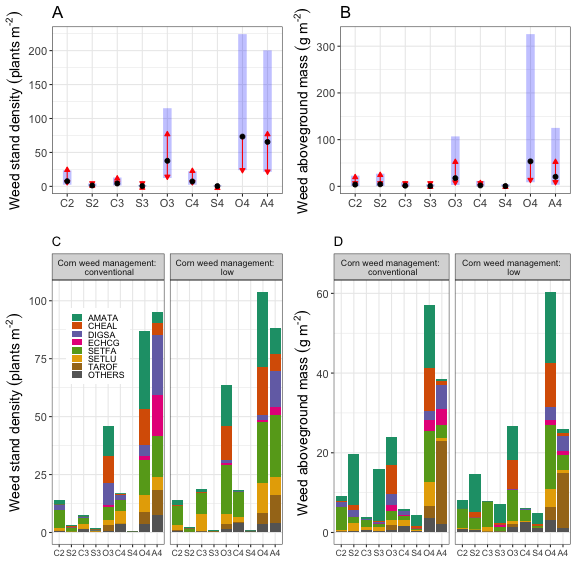
\includegraphics{Community_files/figure-latex/all-sp-dens-biom-1.png}
\caption{\label{fig:all-sp-dens-biom}In panels A and B: weed community stand density and aboveground mass were averaged over four blocks, four years, and two corn weed management regimes; the black dots are estimated marginal means; the blue bars are 95\% confidence intervals; the red arrows reflect the comparisons among means; overlapping arrows indicate non-significant differences. In panels C and D: the contribution of the seven most abundant weed species and the rarer species (species ordered eighth and above grouped in OTHERS) in each crop identity, averaged over four blocks and four years, are ordered alphabetically. The abbreviations on the x-axis are crop identities, which are the combinations of the first letter in crop species names and the rotation in which it occurred (C2 - corn in the 2-year rotation, C3 - corn in the 3-year rotation, C4 - corn in the 4-year rotation, S2 - soybean in the 2-year rotation, S3 - soybean in the 3-year rotation, S4 - soybean in the 4-year rotation, O3 - oat in the 3-year rotation, O4 - oat in the 4-year rotation, and A4 - alfalfa in the 4-year rotation.) The less abundant weed species which made up 6\% of the whole community are grouped in OTHERS. The means displayed on panels A and B were estimated marginal means, calculated based on the analysis model (with \texttt{emmip} function) but the means displayed on panels C and D were arithmetic means, calculated from the data so they are slightly different.}
\end{figure}

\end{document}
